--- add.tex ---
% !TEX root = ../master-thesis.tex

\textbf{From frequency to position}. И в camera based balancing, и в atoms based balancing для обработки изображений удобно определить афинное преобразование из frequency space to position space:
\begin{equation*}
	\vc{r} = H \vc{\omega}
	\hspace{5 mm} \leftrightarrow \hspace{5 mm} 
	\begin{pmatrix}
		x \\ y
	\end{pmatrix} = \begin{pmatrix}
		h_{11} & h_{12} & h_{13} \\
		h_{21} & h_{22} & h_{23} \\
	\end{pmatrix} 
	\begin{pmatrix}
		\sub{\omega}{hor} \\
		\sub{\omega}{ver} \\
		1
	\end{pmatrix}.
\end{equation*}
Можно, например, для случайных $\vc{\omega}_j \in [\sub{\omega}{min},\, \sub{\omega}{max}]$ измерить $\vc{r}_j$, таким образом сформировав две матрицы $\omega_{ij}$ with $i \in \{\mathrm{hor},\, \mathrm{ver}\}$ and $r_{ij}$ with $i \in \{x, y\}$. Остается решить уравнение на $H$ (что соответсвует Least squares method):
\begin{equation}
	r = H \omega,
	\hspace{0.5cm} \Rightarrow \hspace{0.5cm}
	r \omega\T = H \omega \omega\T
	\hspace{0.5cm} \Rightarrow \hspace{0.5cm}
	r \omega\T \left(\omega \omega\T\right)^{-1} = H.
	\label{LinReg:freq2pos}
\end{equation}

--- balancing_tw_arr.tex ---
% !TEX root = ../master-thesis.tex



\grey{It is also possible to calibrate each AOD independently, without relying on an SVD-based approach. This alternative was not tested in the scope of this work. However, it is worth emphasizing that the SVD-based method is guaranteed to work even for double-AOD configurations~[ref], where crosstalk between the two directions can be significantly stronger.}

Precise control over the depth of each optical tweezer is essential for preparing few-fermion systems via spilling techniques. In our setup, each tweezer is initially loaded with approximately \red{100} atoms, which are then selectively removed by ramping down the potential depth. The number of remaining atoms as a function of spill power $x_{\mathrm{sp}}$ exhibits a quantized staircase structure, reflecting the discrete energy levels of the 1D harmonic oscillator. This behavior can be characterized by a step plot~\cite{holten_pauli_2022}.

\textbf{Step plot.}
To characterize this behavior in our tweezer array, we measure step plots for all sites simultaneously. Figure~\ref{fig:stepplot}a shows the result for a $4 \times 4$ array. For each value of $x_{\mathrm{sp}}$, we acquire 70 experimental realizations and compute the average photon signal per site. 
% This signal serves as a robust proxy for atom number. In contrast to single-atom counting, this approach is parameter-free and effective even for large initial occupancies.

\textbf{Uniformity characterization.}
To quantify depth inhomogeneity across the array, we fit each step trace with a sigmoid function:
\begin{equation*}
    \sigmoid(x) = \frac{A_j}{1 + \exp\left(-(x - x_j)/\sigma_j\right)},
\end{equation*}
where $x_j$ denotes the center of the step and $\sigma_j$ its width for tweezer $j$. We define a relative uniformity metric as $\std(x_j) / \langle x_j \rangle$. After camera-based balancing (Sec.~\ref{subsec:control}), this metric typically yields $\sim 3\%$, which is insufficient for deterministic preparation across the array. A more precise balancing procedure is therefore required.




\textbf{Single-value feedback.}
To further improve uniformity, we apply an iterative atom-based feedback scheme. Rather than fitting full step plots, we operate at a single point on the slope of the transition, near the half-filling level $A_j / 2$. At this point, the sigmoid can be approximated by a linear response:
\begin{equation*}
    \sigmoid(x) \approx \frac{A_j}{4 \sigma_j} x - \frac{A_j x_j}{4 \sigma_j},
\end{equation*}
assuming $x_j \gg \sigma_j$.  In the feedback loop, we do not use the fitted sigmoid parameters directly. Instead, we measure a single photon-count matrix $M_{ij}$ and treat it as a linear proxy for the power matrix $P_{ij}$. Since the sigmoid offset $\mathrm{shift} = A_j x_j / (4 \sigma_j)$ is known from the fits, we approximate:
\begin{equation}
    \label{mp-propto}
    M_{ij} + \mathrm{shift} \propto P_{ij} = \Lambda H_i V_j.
\end{equation}
We then factorize this matrix using the method introduced in \eqref{uv-decomposition} and update the amplitudes according to:
\begin{equation*}
    h \rightarrow h + \gamma (H - H_0), \qquad
    v \rightarrow v + \gamma (V - V_0),
\end{equation*}
where $(H_0, V_0)$ is the target point, and $\gamma$ is the feedback rate. This model-free procedure avoids full sigmoid fitting and operates directly on experimental measurements.

Figure~\ref{fig:stepplot}b shows the result of applying this single-value feedback (SVF) protocol to a $4 \times 4$ array. After five iterations, the relative deviation of the fitted step centers is reduced to $0.7(2)\%$, well within the plateau width (typically $\pm5\%$), enabling deterministic state preparation across the full array. \red{Add fig. with single value feedback progress.}

Figure~\ref{fig:svf}a shows the process of applying the SVF protocol to a $6 \times 6$ array. The proportionality coefficient in \eqref{mp-propto} is $A/4\sigma \sim 10(1)$ (the average value is chosen for the plot) for our experiment.

--- bool-dec.tex ---
% !TEX root = ../master-thesis.tex

...

% Мы хотим найти разложение булевой матрицы $W_{ij}$ размера $n\times n$
% \begin{equation*}
% 	W_{ij} = \sum_{\lambda=1}^r u^\lambda_i v^\lambda_j,
% \end{equation*}
% для наименьшего булева ранга $r$ (или bipartite dimension). Всевозможных матриц $\card\{W_{ij}\} = 2^{n^2}$. Для $n \leq 5$ it about 34 miilion states, so it can be decomposed with brute force \red{(ссылка на код)}. \grey{Можно }

% Для больших $n$ можем попробовать подход с flip graph. TBA. 



--- controlling_tw_arr.tex ---
% !TEX root = ../master-thesis.tex

\textbf{Frequency to position mapping.}
To extract the local intensities $P_{ij}$ from camera images, we need to determine which pixels correspond to which tweezer sites. For this purpose, we define an affine transformation from the drive frequency space $(\omega_{\mathrm{hor}}, \omega_{\mathrm{ver}})$ to image plane coordinates $(x, y)$:
\begin{equation*}
    \vc{r} = H \vc{\omega},
    \hspace{5 mm} \Leftrightarrow \hspace{5 mm} 
    \begin{pmatrix}
        x \\ y
    \end{pmatrix} = \begin{pmatrix}
        h_{11} & h_{12} & h_{13} \\
        h_{21} & h_{22} & h_{23}
    \end{pmatrix} 
    \begin{pmatrix}
        \sub{\omega}{hor} \\
        \sub{\omega}{ver} \\
        1
    \end{pmatrix}.
\end{equation*}
Here, $H$ is a $2 \times 3$ matrix calibrated from a set of measured spot positions. For example, one can measure $\vc{r}_j$ for random frequency vectors $\vc{\omega}_j \in [\omega_{\mathrm{min}},\, \omega_{\mathrm{max}}]$, construct the matrices $\omega_{ij}$ with $i \in \{\mathrm{hor}, \mathrm{ver}\}$ and $r_{ij}$ with $i \in \{x, y\}$, and solve the least-squares problem:
\begin{equation}
    r = H \omega,
    \hspace{0.5cm} \Rightarrow \hspace{0.5cm}
    r \omega^\mathrm{T} = H \omega \omega^\mathrm{T}
    \hspace{0.5cm} \Rightarrow \hspace{0.5cm}
    r \omega^\mathrm{T} \left(\omega \omega^\mathrm{T}\right)^{-1} = H.
    \label{eq:linreg-freq2pos}
\end{equation}

This transformation defines a region of interest around each tweezer, within which we compute the integrated pixel intensity after background subtraction. The resulting values are proportional to the optical powers $P_{ij}$.

\textbf{Linear reconstruction.}
The mapping from input amplitudes $\vc{a}$ to optical power is approximated by Eq.~\eqref{eq:taylerexp}. In the regime $a_i \in [0.85, 0.95]$, a linear approximation is sufficient\footnote{
    For wider amplitude ranges, higher-order terms can be added to the model. However, this is unnecessary in the present context.
}. We construct the Jacobian matrix $F'_{ji}$ by fitting a linear regression model to a dataset of amplitude–intensity pairs. The resulting crosstalk matrix is shown in Fig.~\ref{fig:control}b. It is approximately diagonal, with comparable diagonal entries and off-diagonal elements typically reaching up to 30\% in magnitude relative to the diagonal, due to power redistribution between neighboring tones. Crosstalk between the horizontal and vertical AODs remains negligible.

The quality of the linear fit for the $4 \times 4$ array is illustrated in Fig.~\ref{fig:control}e. The total intensity (Fig.~\ref{fig:control}d) scales linearly with the average input amplitude, yielding $R^2 > 0.99$. Relative residuals are normally distributed with width $0.3\%$, confirming the applicability of the model in this range.

\textbf{Power-aware optimization.}
\grey{In the presence of limited laser power and finite AOM diffraction efficiency, we prefer solutions where all amplitudes remain close to 1. This preference can be incorporated into the optimization objective. In addition to minimizing intensity imbalance, we penalize deviations of the average amplitudes from a target value (e.g., 0.9).}



\begin{figure}
    \centering
    \addletter{170}{a}
    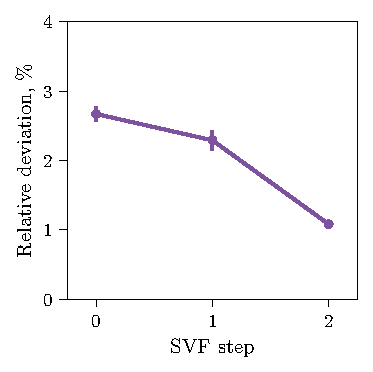
\includegraphics{fig-py/svf-avg.pdf}
    \addletter{170}{b}
    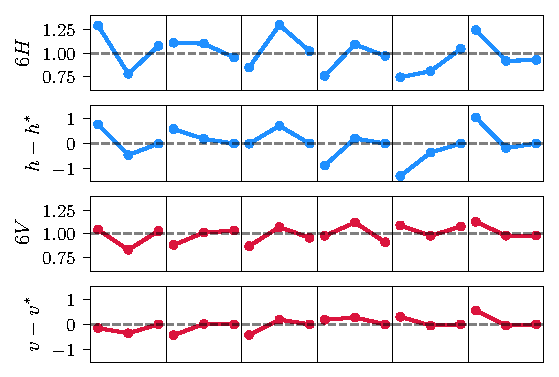
\includegraphics{fig-py/svf.pdf}
    \caption{
        \textbf{Single-value feedback (SVF) optimization for a $6 \times 6$ tweezer array.}
        (a) Relative deviation of effective powers $P_j$ across the array during successive SVF steps, quantified as $\mathrm{std}(P_j)/\langle P_j \rangle$. The initial point corresponds to camera-based balancing; subsequent iterations apply SVF with feedback rates $\gamma = 1/20$ and $\gamma = 1/40$. Further iterations did not yield statistically significant improvements. 
        (b) Retrieved horizontal powers $H_i$ and vertical powers $V_j$ (top and third rows), along with corresponding deviations of driving amplitudes from their final target values, $h - h^*$ and $v - v^*$. The recovered $H$, $V$ vectors are extracted from the photon count matrix $M_{ij}$ using factorization as described in \eqref{uv-decomposition}.
    }
    \label{fig:svf}
\end{figure}

--- exp-setup-fh.tex ---
% !TEX root = ../master-thesis.tex

The Fermi-Hubbard model is a cornerstone theoretical framework for describing strongly correlated electron systems, particularly relevant in condensed matter physics for understanding the behavior of high-temperature superconductors, such as cuprates \cite{koepsell_quantum_2021}. The Hamiltonian of the 2D Fermi-Hubbard model is typically expressed as:
\begin{equation}
H = -t \sum_{\langle i,j \rangle, \sigma} \left( c_{i,\sigma}^\dagger c_{j,\sigma} + \text{h.c.} \right) + U \sum_i n_{i,\uparrow} n_{i,\downarrow} + \sum_{i,\sigma} \varepsilon_i n_{i,\sigma},
\label{eq:fermi-hubbard}
\end{equation}
where the first term represents hopping with amplitude $t$ between nearest-neighbor lattice sites, the second term describes the on-site interaction energy $U$, and the third term introduces site-dependent energy offsets $\varepsilon_i$, accounting for disorder or external potentials \cite{koepsell_quantum_2021}.

In physical terms, the competition between kinetic energy, captured by the hopping term, and potential energy, represented by the on-site interaction, gives rise to rich emergent phenomena. At half-filling and sufficiently large interaction strength $U \gg t$, the model predicts the formation of a Mott insulating phase, characterized by suppressed conductivity due to electron localization. At lower temperatures, antiferromagnetic correlations dominate, leading to spin ordering. Upon doping, the system can exhibit pseudogap behavior and potentially unconventional superconductivity analogous to that observed in cuprates, although achieving clear signatures of superconductivity in numerical and experimental studies remains challenging \cite{koepsell_quantum_2021}.

Beyond the single-layer scenario, the bilayer 2D Fermi-Hubbard model offers additional intriguing phenomena, including enhanced pairing mechanisms and novel magnetic orders. Experimentally realizing such bilayer systems could provide critical insights into mechanisms underlying high-temperature superconductivity. Within the UniRand experiment, employing an accordion lattice geometry makes the exploration of bilayer configurations feasible, thereby opening new avenues for investigating these phenomena \cite{huang_construction_2024}.

In the context of ultracold atoms, the Fermi-Hubbard model can be realized by trapping fermionic atoms, such as $^6$Li, in optical lattices, where parameters of the Hamiltonian can be precisely tuned. Specifically, the interaction parameter $U$ is controlled via Feshbach resonances, where an external magnetic field is adjusted to tune the scattering length between atoms in different hyperfine states. This allows continuous tuning from attractive to strongly repulsive interactions, enabling experimental exploration of the full phase diagram \cite{culemann_construction_2024}.

The hopping amplitude $t$ is controlled by adjusting the depth of the optical lattice potential. Deeper lattices decrease the tunneling rate, effectively increasing the ratio $U/t$ and stabilizing strongly correlated insulating phases. Additionally, site-dependent potentials $\varepsilon_i$ can be introduced via digital micromirror devices (DMD), allowing the controlled introduction of disorder or custom potential landscapes essential for exploring Anderson or many-body localization phenomena.

State preparation is envisioned to proceed via an initial deterministic loading of atoms into optical tweezer arrays, followed by a transfer into optical lattices. Such a procedure offers precise control over initial conditions, vital for exploring complex dynamical processes. Furthermore, measurement protocols incorporating Random Unitary Protocols, involving sequences of local random quenches and subsequent measurements, can yield critical information about the entanglement entropy and many-body coherence, significantly enriching experimental observables \cite{culemann_construction_2024, huang_construction_2024}.

% The experimental setup employed by UniRand, detailed further in subsection \ref{subsec:exp-setup-overview}, follows a standard ultracold atom preparation sequence: atoms emitted from an oven are initially captured and cooled in a two-dimensional magneto-optical trap (2D MOT), then transferred into a three-dimensional MOT (3D MOT). Subsequently, atoms are loaded into an optical dipole trap (ODT), further cooled, and finally transferred into an optical tweezer array for deterministic state preparation. The future integration of optical lattices will complete the experimental realization of the Fermi-Hubbard model and its diverse dynamical phases.


--- exp-setup-overview.tex ---
% !TEX root = ../master-thesis.tex

\begin{figure}
    \centering
    \addletter{85}{a} \phantom{4}
    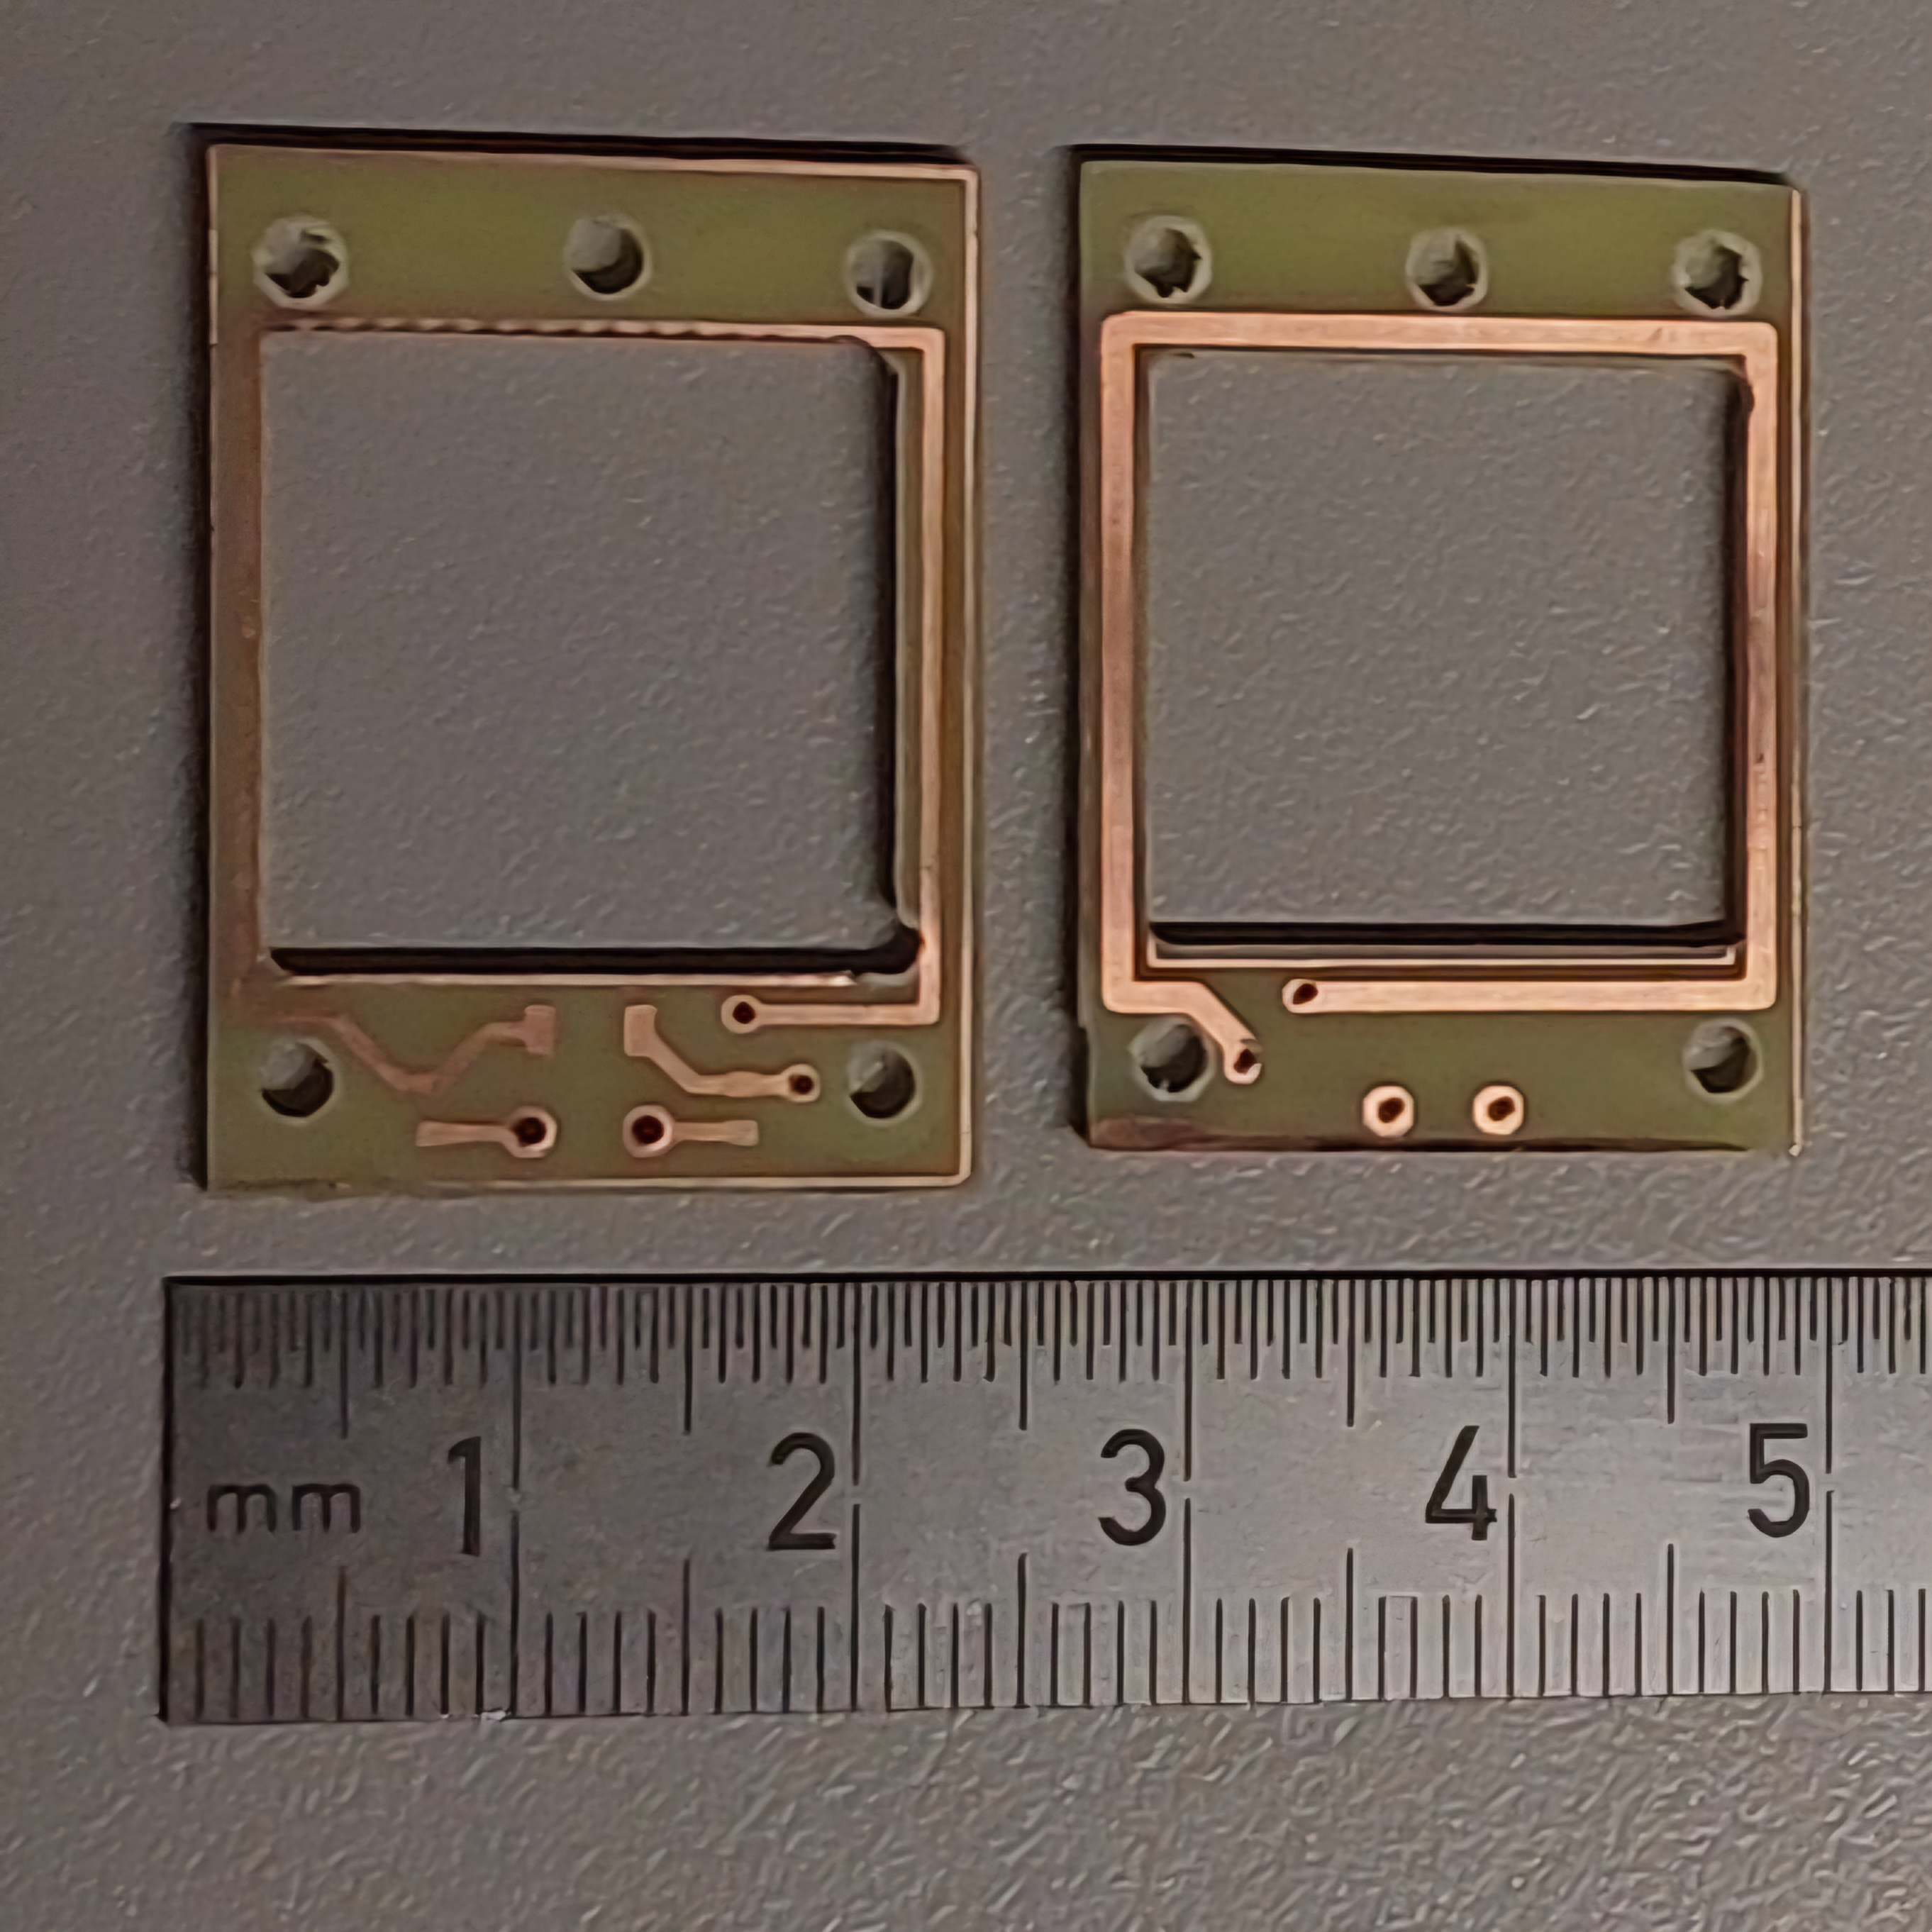
\includegraphics[width=1.25in]{imgs/RF.jpg}
    \hspace{1cm}
    \addletter{85}{b} \phantom{4}
    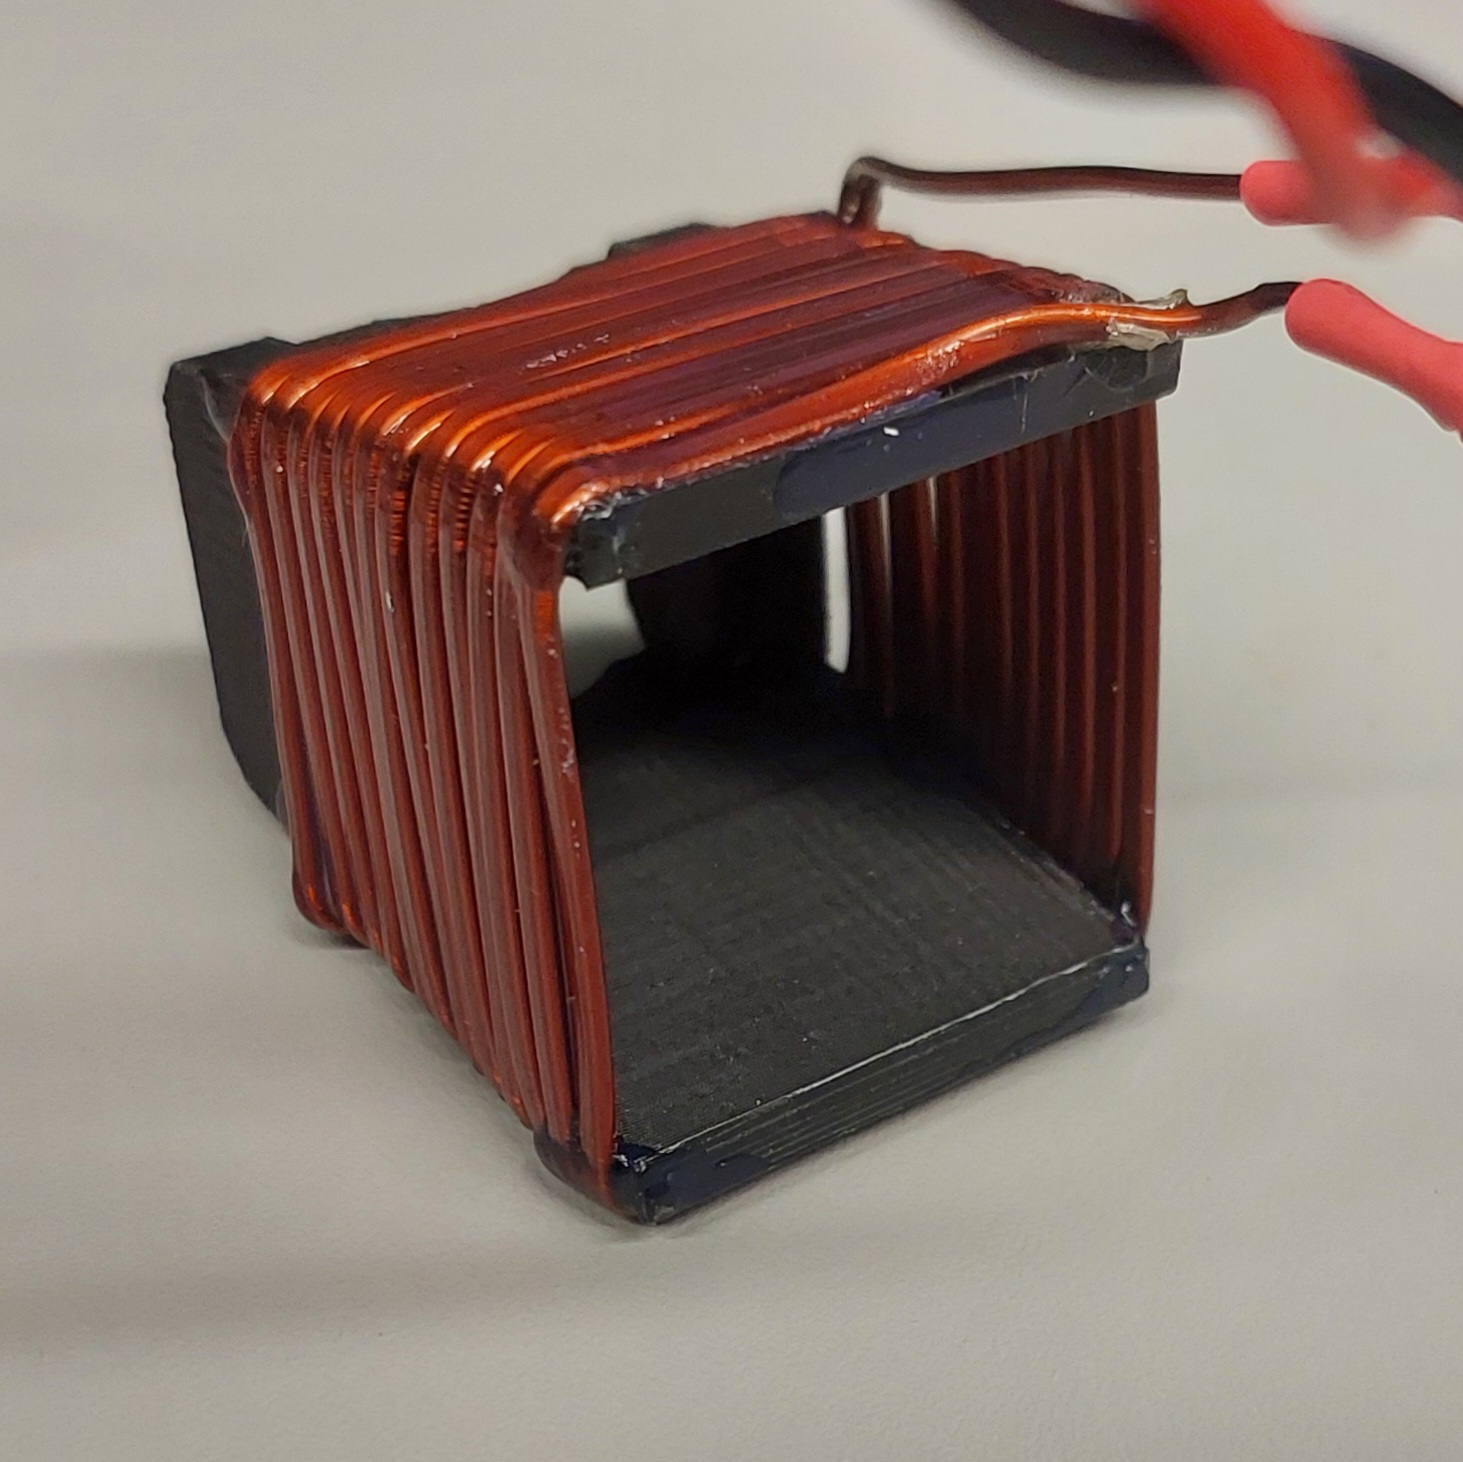
\includegraphics[width=1.25in]{imgs/MW.jpg}
    \caption{
        \textbf{RF and MW antennas used for spin control.}
        (a) PCB-based radiofrequency (RF) antenna used for driving spin transitions at MHz frequencies. 
        (b) Microwave (MW) loop antenna, designed to efficiently couple to hyperfine transitions in $^6$Li. 
        These antennas are used for coherent spin manipulation.
        % performance characterization via spin-flip fidelity is discussed in the following figures.
    }
    \label{fig:rfmw}
\end{figure}


\begin{figure}
    \centering
    \addletter{130}{a}
    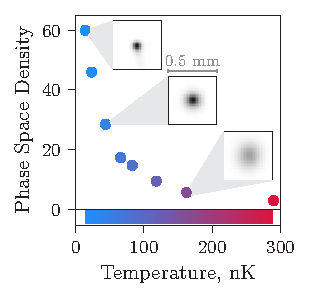
\includegraphics{fig-ai/m-bec-1-joined.pdf}
    \addletter{130}{b}
    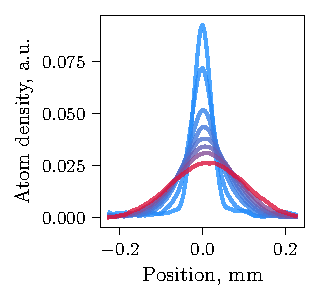
\includegraphics{fig-py/m-bec-2.pdf}
    \addletter{130}{c}
    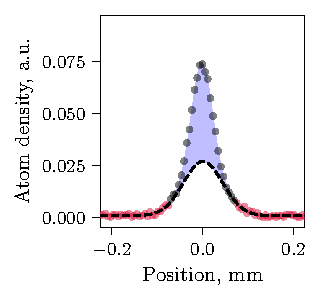
\includegraphics{fig-py/m-bec-3.pdf}
    \caption{
        \textbf{Molecular Bose-Einstein condensate data.}
        (a) Phase space density (PSD) increases as temperature decreases via evaporative cooling, indicating condensation onset. 
        (b) Atom density profiles normalized to unit area; color encodes temperature as in (a).
        (c) At low temperature, the profile shows a bimodal shape: a Gaussian fit to thermal wings (red dots) underestimates the central peak, revealing the mBEC component (blue area).
    }
    \label{fig:mbec}
\end{figure}




\begin{figure}
    \centering
    \addletter{145}{a}
    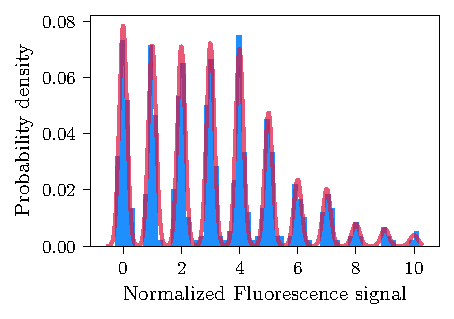
\includegraphics{fig-py/atom-counting.pdf}
    \phantom{4242}
    \addletter{145}{b}
    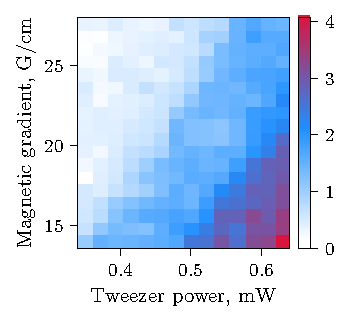
\includegraphics{fig-py/step-plot-2d.pdf}
    \caption{
        (a) Calibration histogram for single-atom counting based on fluorescence signal after after loading to the MOT. Clear quantized peaks correspond to integer atom numbers; the solid red line is a multi-Gaussian fit to the distribution. 
        (b) Measured 2D step plot as a function of tweezer power and magnetic field gradient. Each point indicates the average atom number obtained for a given combination of parameters. This map confirms that for any spill power, a suitable magnetic gradient can be found to achieve a desired quantized atom number.
    }
    \label{fig:spillingadd}
\end{figure}


The UniRand experimental apparatus is designed to realize and investigate complex quantum many-body dynamics using ultracold fermionic $^6$Li atoms. The primary objective of the setup is to create highly controllable initial quantum states, facilitate quantum simulation of the Fermi-Hubbard model, and enable precise measurements of quantum observables, such as entanglement entropy and particle correlations, by employing Random Unitary Protocols \cite{culemann_construction_2024, huang_construction_2024}.

The experimental procedure starts with $^6$Li atoms emitted from an atomic oven. Lithium atoms are first collected and precooled in a two-dimensional magneto-optical trap (2D MOT), effectively capturing a high flux of atoms. From there, the atoms are transferred into a three-dimensional magneto-optical trap (3D MOT) for additional cooling and confinement, reaching temperatures near the Doppler limit (approximately 141~$\mu$K for $^6$Li) \cite{culemann_construction_2024, huang_construction_2024}.

Following the 3D MOT, atoms are loaded into a crossed optical dipole trap (ODT), generated by intersecting laser beams, creating a stable potential. At this stage, evaporative cooling further reduces the temperature significantly below quantum degeneracy conditions, reaching regimes where a molecular Bose-Einstein condensate (mBEC) can form. One of the first tasks within this thesis involved developing software for analyzing mBEC preparation data. Figure~\ref{fig:mbec} illustrates results from this analysis, demonstrating the phase space density (PSD) increasing with reduced temperature due to evaporative cooling (Fig.\ref{fig:mbec}a). Atom density profiles at various temperatures show a characteristic bimodal distribution at low temperatures, indicative of mBEC formation (Fig.\ref{fig:mbec}b). Fitting a Gaussian profile to the thermal wings of this distribution (red points in Fig.\ref{fig:mbec}c) clearly reveals a central peak representing the condensed fraction (blue shaded area in Fig.\ref{fig:mbec}c).

After reaching degeneracy in the ODT, atoms are adiabatically transferred into an optical tweezer array, typically implemented using crossed acousto-optic deflectors (AODs). These tweezers provide deterministic preparation of quantum states with single-site control. Precise atom number management is achieved through the spilling technique, which utilizes a magnetic field gradient and controlled reduction of tweezer depth to selectively retain atoms in low vibrational states \cite{culemann_construction_2024, huang_construction_2024}.

A critical aspect of our experiment is precise atom counting, particularly important when recapturing atoms from tweezers back into the MOT for calibration purposes. Atom number quantization can be clearly observed through fluorescence signal histograms, obtained with prolonged exposure times in a MOT loaded with a small number of atoms. Figure~\ref{fig:spillingadd}a shows discrete peaks corresponding to integer atom numbers, confirming accurate and reliable single-atom counting. 
% Moreover, the measured two-dimensional step plot (Fig.~\ref{fig:spillingadd}b) illustrates how varying tweezer power and magnetic field gradient systematically controls atom number, ensuring high fidelity and repeatability for deterministic state preparation.

Future experimental plans involve transferring precisely prepared atoms into optical lattices engineered to simulate the Fermi-Hubbard model. Lattice depth and geometry, as well as disorder potentials, will be precisely tuned, with disorder introduced using a digital micromirror device (DMD), essential for studying localization phenomena \cite{huang_construction_2024}.

High-resolution, spin-resolved imaging is crucial for detailed characterization of quantum states. Imaging employs fluorescence-based free-space techniques, enabling rapid and high-fidelity spin detection. Atoms are transferred to stretched hyperfine states, optimizing photon collection efficiency through closed cycling transitions.

Control over atomic spin states is executed using dedicated radiofrequency (RF) and microwave (MW) antennas, shown in Fig.\ref{fig:rfmw}. The PCB-based RF antenna (Fig.\ref{fig:rfmw}a) drives MHz-range spin transitions, while the MW loop antenna (Fig.~\ref{fig:rfmw}b) efficiently couples to hyperfine transitions, enabling coherent manipulation critical for state preparation, spin-selective procedures, and precise quantum control.

The entire experimental cycle—including state preparation, evolution, and measurement—is optimized for rapid ( cycle time is about 2s) and reliable repetition, allowing statistically robust data collection. 

--- exp-setup.tex ---
% !TEX root = ../master-thesis.tex

\begin{figure}[htb]
    \centering
    \addletter{200}{a}
    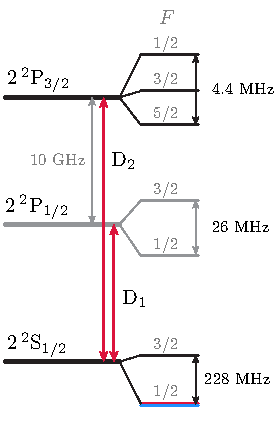
\includegraphics{fig-ai/li-levels-base.pdf}
    \hspace{1cm}
    \addletter{200}{b}
    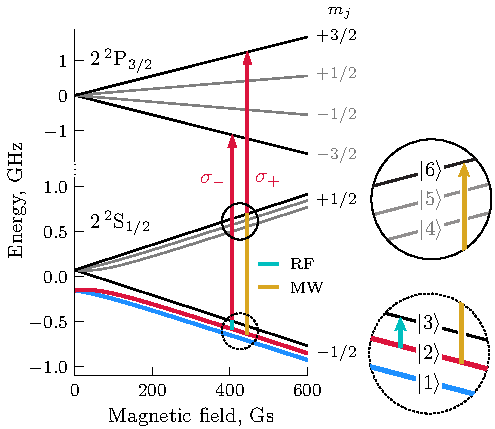
\includegraphics{fig-ai/li6-zeeman-broken-ai.pdf}
    \caption{
        \textbf{${}^6$Li energy levels}. 
        a) Level diagram of the ground and excited states of ${}^6$Li \cite{gehm_preparation_2003}, including the D1 and D2 transitions around $\lambda = 671$~nm. 
        b) Zeeman splitting of the hyperfine levels of the $2\, {}^2\mathrm{S}_{1/2}$ and $2\, {}^2\mathrm{P}_{2/2}$ in ${}^6$Li \cite{serwane_deterministic_2011, sibalic_arc_2017}. As different spin states for physics we consider state $\ket{1}$ and $\ket{2}$, but for imaging it is worth to flip them to stretched states $\ket{6}$, $\ket{3}$. Colored lines indicate transitions driven by radiofrequency (RF) and microwave (MW) fields.
    }
    \label{fig:li6levels}
\end{figure}


--- fh-model-code.tex ---
% !TEX root = ../master-thesis.tex


% А тут расскажу про модель, которую сделал и что мы можем в нашем эксперименте наблюдать. 



% The entanglement entropy between two halves of a $4 \times 4$ Fermi-Hubbard system with $N_\uparrow = N_\downarrow = 2$ is bounded by the logarithm of the Schmidt rank of the reduced density matrix $\rho^A$. Due to particle number conservation, $\rho^A$ decomposes into orthogonal blocks labeled by $(N_\uparrow^{(A)}, N_\downarrow^{(A)}) = (k, l)$. The maximal rank of each block is given by the minimal dimension of the matching sectors in subsystems $A$ and $B$. Thus, the total maximal rank is

% \begin{equation*}
% R_{\max} = \sum_{k=0}^2 \sum_{l=0}^2 \min\left[ \binom{8}{k} \binom{8}{l}, \binom{8}{2-k} \binom{8}{2-l} \right] = 154.
% \end{equation*}

% The corresponding maximal entropy is

% \begin{equation*}
% S_{\max} = \ln(R_{\max}) = \ln(154) \approx 5.04.
% \end{equation*}


% cuda (A100):

% dim=1.44 * 10^4, 28ms на создание гамильтониана;  (N_up=N_down=2)
% 	для 100 сингулярных значения в random SVD: 24ms
% 	ED: 3.5s на диагонализацию : + 0.8ms на вычисление psi в момент времени t; 
% 	Krylov: 8ms на step -- получение psi в следующий момент времени; 

% dim=3.3124 * 10^6, 59ms на создание гамильтониана; (N_up=N_down=4)
% 	для 100 сингулярных значения в random SVD: 4.7s
% 	Krylov: 17ms на step (with K=5); 33ms на step (with K=10)

% dim=1.656369 * 10^8, 110ms на создание гамильтониана; (N_up=N_down=8)
% 	Krylov: 1.06s на step (with K=5); 2.1s на step (with K=10)



% cpu (Intel Xeon Gold 6330):

% dim=3.3124 * 10^6, 93ms на создание гамильтониана; (N_up=N_down=4)
% 	для 100 сингулярных значения в random SVD: 32s
% 	Krylov: 0.708s на step (with K=5); 1.45s на step (with K=10)



% \textbf{Algorithmic implementation}.
The numerical toolbox is designed to simulate dynamics governed by the Fermi-Hubbard Hamiltonian on arbitrary lattice geometries. The Hamiltonian considered is generally given by \eqref{eq:fh-mbl}. At the core of the implementation is the compact representation of fermionic many-body states using bitwise encoding. Specifically, the occupation number of each lattice site by spin-up and spin-down fermions is stored in two separate binary integers, significantly reducing memory consumption and enhancing computational speed. Each basis state is thus represented as a pair of bit patterns, enabling rapid evaluation of physical operators via bitwise logic. The numbers of spin-up particles, $N_\uparrow$, and spin-down particles, $N_\downarrow$, are considered to be conserved.


Performance benchmarks of the numerical toolbox were obtained on a GPU (NVIDIA A100 GPU) for a representative 4×4 lattice system. Benchmark results are summarized in Table~\ref{tab:performance}. For comparison, equivalent calculations performed on a CPU (Intel Xeon Gold 6330) were typically about 40 times slower than those performed on the GPU, underscoring the benefits of GPU acceleration.

\begin{table}
\centering
\caption{
\textbf{Performance benchmarks} (4×4 system, GPU NVIDIA A100).
Execution times correspond to Krylov subspace dimension $K=10$. Columns denote particle numbers $N_\uparrow$, $N_\downarrow$, Hilbert-space dimension $\mathcal{N}$, Hamiltonian construction time $T_H$, Krylov evolution step time $T_{\mathrm{step}}$, entanglement entropy estimation time via randomized SVD $T_{\mathrm{SVD}}$, and exact diagonalization time $T_{\mathrm{ED}}$.
}
\begin{tabular}{ccccccc}
\toprule
$N_\uparrow$ & $N_\downarrow$ & $\mathcal{N}$ & $T_H$ & $T_{\mathrm{step}}$ & $T_{\mathrm{SVD}}$ & $T_{\mathrm{ED}}$ \\
\midrule
2 & 2 & $1.44\times10^4$ & 28 ms & 8 ms & 24 ms & 3.5 s \\
4 & 4 & $3.31\times10^6$ & 59 ms & 33 ms & 4.7 s & N/A \\
8 & 8 & $1.66\times10^8$ & 110 ms & 2.1 s & N/A & N/A \\
\bottomrule
\end{tabular}
\label{tab:performance}
\end{table}

These benchmarks demonstrate that the numerical implementation efficiently scales to large Hilbert-space dimensions, facilitating studies of complex quantum dynamics in regimes beyond reach of exact diagonalization approaches. Krylov subspace methods, combined with optimized GPU execution, ensure that simulations remain computationally feasible even for Hilbert-space sizes on the order of $10^8$ or greater.

% The Hamiltonian is constructed in three parts (kinetic, interaction, and potential terms). The kinetic (hopping) operator is constructed using an adjacency matrix defining the connectivity of the lattice. Hopping processes between sites, exploiting parity counting of intermediate occupied sites to maintain correct fermionic signs during state transitions. The interaction operator, corresponding to the on-site Coulomb repulsion $U$, is implemented by directly counting overlapping occupied sites in the spin-up and spin-down bit patterns.

% Additionally, significant optimization is achieved by leveraging the sparsity of the Hamiltonian. Instead of storing and diagonalizing the Hamiltonian explicitly in full dense form, it is stored in a sparse format suitable for both exact diagonalization (ED) and iterative Krylov-based methods. The Krylov method efficiently approximates the action of the Hamiltonian operator on a state, significantly reducing memory requirements and computational time compared to full diagonalization. This allows simulations of much larger system sizes and longer evolution times.

% The implementation is modular, facilitating easy adjustments or extensions, such as modifying lattice structures or introducing additional Hamiltonian terms.



% To complement and guide the experimental investigations described above, a custom numerical toolbox was developed, specifically tailored for efficient and scalable simulations of real-time quantum dynamics in finite two-dimensional Fermi-Hubbard systems. The main objective of this numerical framework is to provide robust theoretical support, enabling direct comparison between numerical simulations and experimental observations. In particular, the package is optimized for the simulation of unitary quantum dynamics in large Hilbert spaces, with special attention given to computational efficiency and flexibility in system geometry and parameters.

% \textbf{Structure and key optimizations.}
% The core numerical object is the Hamiltonian class, which represents the Fermi-Hubbard Hamiltonian on arbitrary two-dimensional lattice geometries with specified parameters, including hopping amplitude $t$, on-site interaction strength $U$, and local disorder potential $V_i$hamiltonian. Internally, states are represented using compact bitwise encoding for spin-up and spin-down occupation numbers, significantly reducing memory requirements and computation time. Hamiltonian matrix elements—kinetic hopping terms, on-site interaction, and potential energies—are constructed efficiently through bitwise operations and sparse representations, enabling rapid matrix-vector multiplication without explicitly forming large matrices.

% The Hamiltonian's action on wavefunctions ($\psi$) is optimized by separately handling diagonal (interaction and potential) and off-diagonal (hopping) contributions. Specifically, hopping terms are precomputed and stored in sparse formats, allowing efficient parallel execution on GPU. This sparse structure, combined with bitwise state representations, ensures both memory efficiency and computational performance, particularly crucial for large Hilbert spaces.

% \textbf{Krylov-based time evolution.}
% To simulate unitary dynamics, the Krylov subspace projection method (Lanczos-type algorithm) is employed. Instead of explicitly exponentiating the Hamiltonian, the method constructs a Krylov subspace by iteratively applying the Hamiltonian operator to the initial state. The matrix exponential is then computed within this reduced subspace, drastically reducing computational complexity. The accuracy and computational cost of the Krylov approach are controlled by the Krylov dimension parameter ($K$), typically set to around 10 steps for optimal balance between precision and speedkrylov.

% \textbf{Performance benchmarks.}
% Extensive benchmarking on high-performance GPU (NVIDIA A100) demonstrates the numerical toolbox's efficiency and scalability. Table~\ref{tab:performance} summarizes typical execution times for system initialization, Hamiltonian construction, time-evolution steps (via Krylov), and entanglement entropy calculation using randomized SVD. It highlights excellent scalability with Hilbert-space dimension ($\mathcal{N}$), making realistic simulation of experimentally relevant systems feasible. For reference, CPU performance is roughly 40 times slower.

% \begin{table}
% \centering
% \caption{
% \textbf{Performance benchmarks of numerical simulations.} (4×4 system, GPU NVIDIA A100)
% Execution times listed correspond to Krylov dimension $K=10$.
% }
% \begin{tabular}{ccccccc}
% \toprule
% $N_\uparrow$ & $N_\downarrow$ & $\mathcal{N}$ & Hamiltonian construction & Krylov step & Entropy calculation (100 singular values) & ED diagonalization \\
% \midrule
% 2 & 2 & $1.44\times10^4$ & 28 ms & 8 ms & 24 ms & 3.5 s \\
% 4 & 4 & $3.31\times10^6$ & 59 ms & 33 ms & 4.7 s & N/A \\
% 8 & 8 & $1.66\times10^8$ & 110 ms & 2.1 s & N/A & N/A \\
% \bottomrule
% \end{tabular}
% \label{tab:performance}
% \end{table}

% \textbf{Usage and flexibility.}
% The toolbox is designed with modularity and ease of use in mind. Users can conveniently specify system size, particle number, lattice geometry (through adjacency matrices), interaction strength, disorder configurations, and initial states using high-level Python functions. Once defined, time evolution and measurements of observables such as particle densities $\langle n_j(t) \rangle$, local magnetization $\langle \sigma_j^z(t)\rangle$, and entanglement entropy can be performed efficiently.

% \textbf{Illustrative numerical experiment.}
% To demonstrate the toolbox capabilities, consider a specific numerical experiment aimed at distinguishing dynamical phases discussed earlier: thermalization (ETH), Anderson localization (AL), and many-body localization (MBL). Initially, spin-up and spin-down fermions are placed deterministically in opposite corners of a $4\times4$ lattice. The evolution of particle density $\langle n_j(t)\rangle$, local magnetization $\langle \sigma_j^z(t)\rangle$, and entanglement entropy is then computed, averaged over multiple disorder realizations (see Fig.~\ref{fig:loctherm}).

% Tracking average particle density alone ($\langle n_j\rangle$) effectively distinguishes thermalization from localization: density rapidly homogenizes in the ETH regime, while remaining strongly localized under AL and MBL conditions. However, density alone does not clearly differentiate between AL and MBL; both appear similar, with differences becoming apparent only at intermediate disorder strengths due to interaction-induced delocalization in MBL.

% In contrast, local magnetization $\langle \sigma_j^z(t)\rangle$ provides a more sensitive indicator. In Anderson localization, initial magnetization patterns persist indefinitely, whereas interactions in the MBL regime cause the spin configuration to relax despite persistent localization in particle density. Thus, magnetization dynamics clearly separates AL from MBL phases.

% Similarly, the evolution of entanglement entropy exhibits markedly different behavior across phases. In the absence of interactions (AL), entanglement entropy remains bounded at short time scales. In contrast, even weak interactions lead to a characteristic logarithmic growth of entanglement entropy, indicative of MBL dynamics. In fully thermalizing systems, entanglement entropy grows rapidly and saturates at a high value determined by subsystem size and energy density.

% These numerical experiments, enabled by the developed toolbox, directly inform and guide experimental observations. They highlight how carefully chosen observables, combined with deterministic state initialization, can robustly distinguish different dynamical regimes in two-dimensional Fermi-Hubbard systems, thereby linking theory, numerics, and experiment.



--- fh-model-dynamics.tex ---
% !TEX root = ../master-thesis.tex




\begin{figure}
    \centering
    % 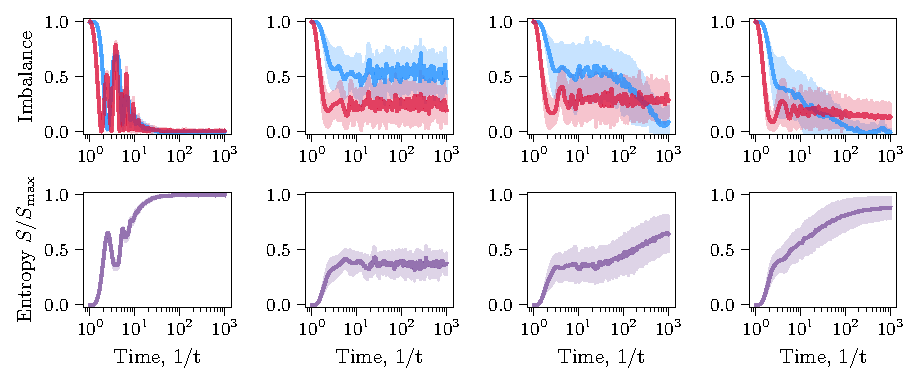
\includegraphics{fig-py/loc-therm.pdf}
    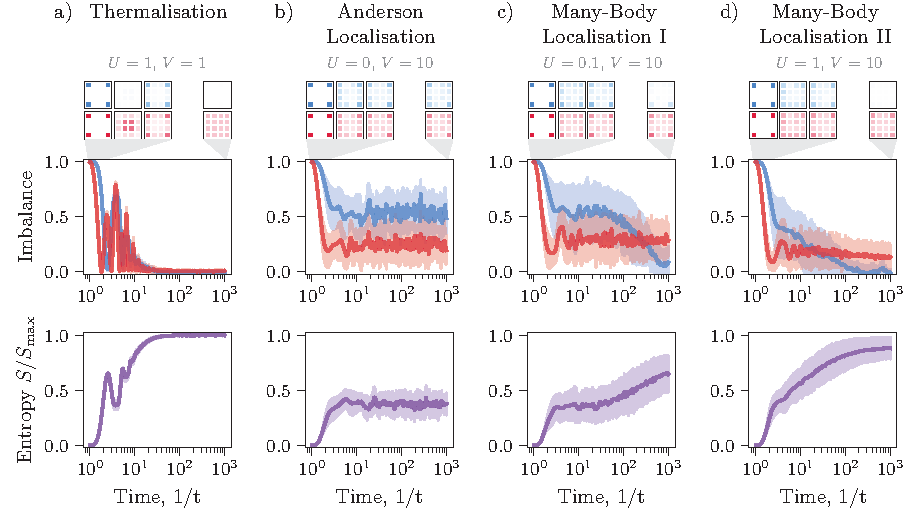
\includegraphics{fig-ai/loc-therm.pdf}
    \caption{
        \textbf{Dynamical phases in a 2D Fermi-Hubbard system.} 
        \textit{Top}: Snapshots of particle density (red) and magnetization magnitude (blue). 
        \textit{Middle}: Time evolution of density imbalance (red) between corners and bulk, and subsystem magnetization (blue). 
        \textit{Bottom}: Normalized entanglement entropy evolution. 
        All results are averaged over 10 noise realizations; shaded areas indicate standard deviation across realizations.
        Data were obtained using ED.
        % Parameters: (a) $U=1, V=1$, (b) $U=0, V=10$, (c) $U=0.1, V=10$, (d) $U=1, V=10$.
        % \\ \textit{Parameters:} (a) $(1,1)$, (b) $(0,10)$, (c) $(0.1,10)$, (d) $(1,10)$ for $(U,V)$.
    }
    \label{fig:loctherm}
\end{figure}

A key application of the numerical simulation toolbox developed in this work is the systematic exploration and clear identification of dynamical phases in interacting fermionic systems, described by the Fermi-Hubbard Hamiltonian. To illustrate this capability, a concrete numerical experiment is considered here, focusing on distinguishing between three distinct dynamical regimes: thermalization governed by Eigenstate Thermalization Hypothesis (ETH), Anderson localization, and many-body localization (MBL). The main motivation for this numerical investigation is to demonstrate explicitly how carefully chosen initial states and targeted observables facilitate clear experimental signatures distinguishing these different phases.

\textbf{Initial state and experimental setup.}
The initial condition selected for this numerical experiment involves a spatially separated arrangement of spin-up and spin-down fermions in a two-dimensional lattice geometry. Specifically, the initial wavefunction is prepared with spin-up fermions localized at two diagonally opposite corners of the lattice, and spin-down fermions positioned at the other two corners. This arrangement generates an initial maximal density imbalance between the corners and the lattice bulk, accompanied by a similarly maximal spin imbalance across the system. This choice of initial condition serves two main purposes. First, it creates a strongly non-equilibrium state that provides clear initial reference points for monitoring relaxation dynamics. Second, it allows separate and simultaneous tracking of particle density and spin distribution, thus providing additional insights into the many-body processes at play.

The Hamiltonian parameters considered in this experiment vary across three physically relevant regimes. In particular, the interaction strength $U$ and disorder strength $V$ are systematically tuned to access the thermalization, Anderson localization, and many-body localization regimes. Simulations are performed using exact diagonalization 
% for moderate system sizes and verified by employing Krylov subspace methods for larger Hilbert-space dimensions. 
For reliable statistics, the results reported in this numerical experiment are averaged over ten independent disorder realizations.

% \begin{figure}
%     \centering
%     % 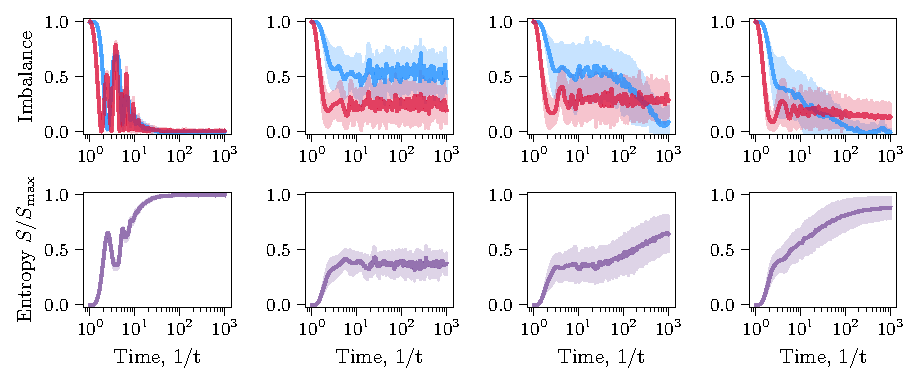
\includegraphics{fig-py/loc-therm.pdf}
%     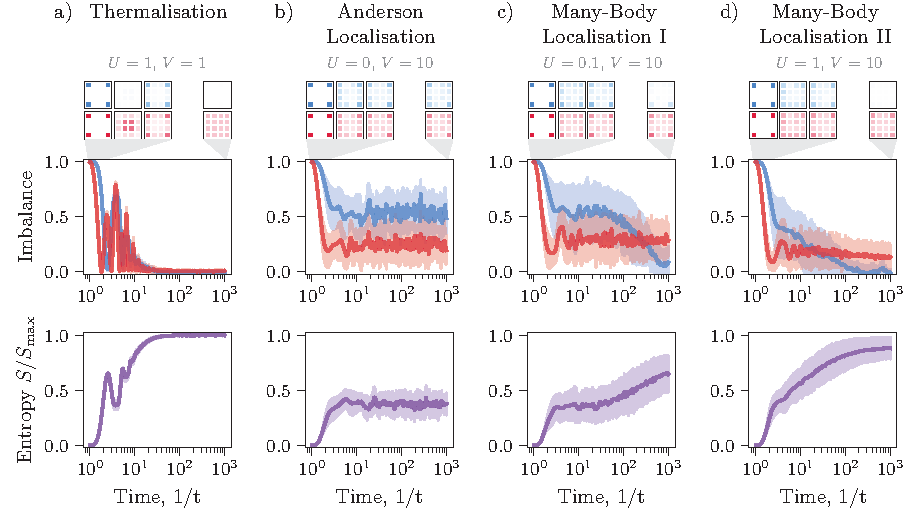
\includegraphics{fig-ai/loc-therm.pdf}
%     \caption{
%         \textbf{Dynamical phases in a 2D Fermi-Hubbard system.} 
%         \textit{Top}: Snapshots of particle density (red) and magnetization magnitude (blue). 
%         \textit{Middle}: Time evolution of density imbalance (red) between corners and bulk, and subsystem magnetization (blue). 
%         \textit{Bottom}: Normalized entanglement entropy evolution. 
%         All results are averaged over 10 noise realizations; shaded areas indicate standard deviation across realizations.
%         Data were obtained using ED.
%         % Parameters: (a) $U=1, V=1$, (b) $U=0, V=10$, (c) $U=0.1, V=10$, (d) $U=1, V=10$.
%         % \\ \textit{Parameters:} (a) $(1,1)$, (b) $(0,10)$, (c) $(0.1,10)$, (d) $(1,10)$ for $(U,V)$.
%     }
%     \label{fig:loctherm}
% \end{figure}


\textbf{Observables and their physical significance.}
Three primary observables are investigated in this numerical experiment to characterize and distinguish among the dynamical phases mentioned above. The first observable is the particle density imbalance, defined as the normalized difference between particle densities at initially occupied corner sites and the bulk sites. Formally, this imbalance can be expressed as
\begin{equation}
\mathcal{I}(t) = \frac{N_\text{corner}(t)-N_\text{bulk}(t)}{N_\text{corner}(t)+N_\text{bulk}(t)},
\end{equation}
where $N_\text{corner}(t)$ and $N_\text{bulk}(t)$ represent particle numbers at corner and bulk sites, respectively, at time $t$. This observable is sensitive to particle redistribution across the lattice, clearly distinguishing thermalization (complete imbalance relaxation), Anderson localization (persistent imbalance), and intermediate behavior in MBL.

The second observable investigated is the subsystem magnetization $\langle \sigma_j^z\rangle$, representing local spin polarization at individual lattice sites. Unlike particle density imbalance alone, magnetization provides further crucial differentiation between Anderson localization, where spin distributions remain essentially static due to absence of interactions, and MBL or thermalization regimes, where spins dynamically rearrange due to interactions.

The third observable employed is the bipartite entanglement entropy, defined by partitioning the lattice system into two equal subsystems. This entropy provides direct insight into the correlation dynamics and quantum information propagation in the system, with characteristic signatures distinctly differentiating ETH, Anderson localization, and MBL phases.

% \textbf{Results and interpretation of numerical simulations.}
The numerical results of this illustrative experiment are summarized in Fig.~\ref{fig:loctherm}. These simulations clearly demonstrate distinct behavior across different regimes, highlighting the utility of the numerical toolbox in characterizing these dynamical phases.


\textbf{Thermalization regime (ETH).}
For parameters corresponding to moderate interaction strength and weak disorder ($U=1$, $V=1$), the numerical results show rapid and complete relaxation of the particle density imbalance to zero, indicating full particle redistribution throughout the lattice. Simultaneously, the subsystem magnetization vanishes on similarly short timescales, clearly reflecting efficient spin mixing driven by interactions. The entanglement entropy exhibits rapid initial growth, quickly reaching saturation at values approaching maximal entropy for the subsystem. These dynamical signatures precisely match theoretical predictions from the ETH framework, wherein local observables lose memory of initial conditions and approach thermodynamic equilibrium at late times \cite{deutsch_quantum_1991,srednicki_chaos_1994}.

\textbf{Anderson localization regime.}
In contrast, the numerical simulations at zero interaction and strong disorder strength ($U=0$, $V=10$) demonstrate distinct dynamical signatures characteristic of Anderson localization. The particle density imbalance remains nearly constant throughout the time evolution, showing negligible redistribution of particles from initial localized positions. Furthermore, subsystem magnetization remains stable, indicating minimal spin rearrangements. Crucially, the entanglement entropy shows almost no growth, stabilizing at values near zero, indicative of the absence of significant entanglement generation. These results clearly align with the theoretical expectation of Anderson localization, where the absence of interactions ensures persistence of initial conditions indefinitely \cite{anderson_absence_1958,abrahams_50_2010}.

\textbf{Many-body localization regime.}
For finite interactions in a strongly disordered environment ($U=0.1$ or $U=1$, with $V=10$), the numerical simulations show the hallmark features of many-body localization. In this regime, the particle imbalance partially relaxes but stabilizes at a finite nonzero value, signifying the suppression but not complete absence of transport. In sharp contrast to Anderson localization, the subsystem magnetization gradually diminishes over time, reflecting slow spin thermalization due to interactions, despite the presence of disorder. Most importantly, the entanglement entropy in this regime exhibits a slow, logarithmic increase without saturating quickly, distinguishing MBL from the other phases clearly. This slow entanglement growth is a distinct theoretical signature of MBL and arises fundamentally from interactions and dephasing processes absent in non-interacting localization scenarios \cite{basko_metalinsulator_2006,nandkishore_many-body_2015}.

% \textbf{Experimental relevance and further perspectives.}
% The presented numerical results clearly illustrate the feasibility of using carefully designed initial states and targeted observables to distinguish experimentally among ETH, Anderson localization, and MBL phases. In particular, the combination of particle density, spin magnetization, and entanglement entropy measurements provides a comprehensive experimental protocol that could be readily implemented in quantum gas microscope experiments or tweezer arrays, such as those considered in the experimental part of this thesis.

% The numerical simulations further guide experimental efforts by predicting observable timescales and characteristic signatures for each phase, thus aiding in the optimal design of measurement protocols. In particular, direct experimental access to local density and spin distributions, combined with recently developed experimental methods for measuring entanglement entropy (e.g., via randomized unitaries), provides a realistic pathway toward direct verification of these theoretical predictions.

% Moreover, the flexibility of the numerical toolbox allows future studies to easily extend these numerical experiments to larger system sizes, different lattice geometries, additional Hamiltonian terms, or modified initial states. Such extensions would significantly enrich the understanding of non-equilibrium quantum dynamics and contribute further to theoretical and experimental explorations of interacting quantum many-body systems.

% In conclusion, this illustrative numerical experiment effectively demonstrates the capability of the developed numerical toolbox to identify and characterize distinct dynamical phases in the Fermi-Hubbard model. Through systematic variation of initial conditions and Hamiltonian parameters, the numerical simulations yield clear and experimentally testable predictions, thus bridging theoretical predictions and experimental realizations in quantum many-body physics.


\textbf{Experimental relevance and further perspectives.}
The presented numerical results illustrate the feasibility of using carefully designed initial states and targeted observables to experimentally distinguish among ETH, Anderson localization, and MBL phases. In particular, simultaneous measurements of particle density, spin magnetization, and entanglement entropy can be directly implemented in experimental setups such as quantum gas microscopes or tweezer arrays, as discussed in previous sections.

Numerical simulations predict characteristic timescales and clear observable signatures for each dynamical phase, providing concrete guidelines for experimental protocols. Furthermore, recently developed experimental methods for measuring entanglement entropy, such as randomized unitaries, offer realistic pathways for direct verification of theoretical predictions.









--- fh-model-intro.tex ---
% !TEX root = ../master-thesis.tex

% --------------------------------------------------------------------------------------
% Intro
% --------------------------------------------------------------------------------------

% \textbf{Overview.}
Understanding the dynamics of isolated quantum systems remains one of the central goals of contemporary many-body physics. Over the last decades, considerable progress has been made in classifying and probing different dynamical regimes, from thermalizing phases consistent with conventional statistical mechanics to exotic non-ergodic phases that violate the Eigenstate Thermalization Hypothesis (ETH). Among these, the Fermi-Hubbard model has emerged as a paradigmatic platform for studying the interplay of interactions, quantum statistics, and disorder in strongly correlated systems.

In the clean, disorder-free limit, the Fermi-Hubbard model exhibits rich equilibrium physics, including Mott insulators, spin ordering, and pseudogap phenomena relevant to high-temperature superconductivity \cite{esslinger_fermi-hubbard_2010}. However, the model also serves as a fertile ground for exploring nonequilibrium phenomena, such as quantum quenches, relaxation, transport, and entanglement dynamics — especially when generalized to include disorder or spatial inhomogeneities.

Recently, theoretical and experimental attention has increasingly shifted toward the role of disorder in quantum many-body dynamics. It is now understood that disorder can lead to fundamentally different behaviors depending on the presence or absence of interactions. For instance:
\begin{itemize}
	\item In the absence of interactions, disorder induces \textit{Anderson localization}, which prevents particle diffusion and leads to persistent memory of initial conditions \cite{anderson_absence_1958}.
	\item When interactions are present, the system may enter the regime of \textit{many-body localization (MBL)}, characterized by the absence of thermalization and slow unbounded entanglement growth \cite{basko_metalinsulator_2006,nandkishore_many-body_2015}.
	% , and emergent local integrals of motion
	\item In contrast, when disorder is weak or absent, the system typically evolves toward local thermal equilibrium, consistent with the predictions of \textit{ETH} \cite{deutsch_quantum_1991,srednicki_chaos_1994}. 
\end{itemize}

These dynamical phases (\emph{thermal, Anderson-localized, and MBL}) are typically distinguished through the behavior of local observables, spectral statistics, and the dynamics of quantum correlations. Their interplay is especially rich in two dimensions, where the presence of more complex geometry, potential mobility edges, and rare-region effects make the dynamical phase diagram both challenging and intriguing.

From an experimental standpoint, studying such phenomena requires precise control over initial states, evolution Hamiltonians, and high-fidelity measurements of observables at the single-site level. This thesis presents a platform that provides such control, combining deterministic initialization of fermionic states in a two-dimensional tweezer array with programmable evolution under the Fermi-Hubbard Hamiltonian and spin- and site-resolved imaging.

Compared to conventional optical lattice experiments, the tweezer-based approach offers several key advantages for nonequilibrium quantum simulation:
\begin{enumerate}
	\item \textit{Deterministic and programmable state preparation.} Using a sequence of global and spin-selective spilling operations, arbitrary configurations of fermionic atoms can be prepared with high fidelity. This capability enables initialization of tailored many-body states for probing specific dynamical scenarios, such as local quenches, domain-wall melting, or imbalance relaxation.
	\item \textit{Fast experimental cycle and large statistics.} The entire experimental sequence, including preparation, evolution, and measurement, completes in under two seconds, allowing up to $10^5$ experimental repetitions per day. This rapid repetition rate is crucial for averaging over disorder realizations and collecting sufficient statistics for dynamical observables.
	\item \textit{Spin- and site-resolved detection.} The developed imaging system supports fluorescence-based, single-shot discrimination of atomic spin states on individual lattice sites. This enables direct access to observables such as density profiles $\langle n_j \rangle$, magnetization $\langle \sigma^z_j \rangle$, and spin correlations $\langle \sigma^z_i \sigma^z_j \rangle$ — all of which are sensitive to the system's dynamical regime.
\end{enumerate}

In tandem with experimental capabilities, in this work a numerical simulation package was developed for modeling real-time dynamics in finite-size Hubbard systems. The package combines exact diagonalization (ED) for small systems and Krylov subspace methods for larger Hilbert spaces (up to $10^9$ dimensions), and supports evaluation of observables and entanglement entropy in arbitrary geometries and disorder realizations.

Together, these tools enable a systematic exploration of the dynamical phase diagram of the disordered Fermi-Hubbard model in two dimensions. By leveraging control over initial conditions, disorder strength, and interactions, as well as the ability to access key observables, one can address central questions in nonequilibrium many-body physics: What determines whether a system thermalizes? When does localization persist in the presence of interactions? How do correlations and entanglement spread in different regimes?

In the following subsections, we review the theoretical framework underpinning these questions, beginning with the concept of thermalization in isolated quantum systems.



--- fh-model-methods.tex ---
% !TEX root = ../master-thesis.tex


Experimental investigation of quantum many-body dynamics benefits greatly from accurate and scalable numerical modeling. In the context of disordered Fermi-Hubbard systems, such modeling helps in validating measurement protocols and benchmarking physical observables. However, simulating out-of-equilibrium dynamics in two-dimensional systems remains a formidable task due to the exponential growth of the Hilbert space with system size and the rapid entanglement generation in thermalizing regimes.

To address these challenges, a numerical framework was developed in the course of this work. It supports efficient simulation of unitary dynamics in finite two-dimensional Fermi-Hubbard systems with arbitrary geometries, boundary conditions, and disorder realizations. The framework combines two complementary computational strategies:

\textit{Exact diagonalization (ED).}
For systems with Hilbert space dimension up to $\mathcal{N} \sim 10^4$, full diagonalization of the Hamiltonian $\hat{H}$ allows direct computation of all eigenvalues ${\varepsilon_j}$ and eigenstates ${\ket{E_j}}$. Time evolution of an initial state $\ket{\psi_0}$ is then given by:
\begin{equation}
\ket{\psi(t)} = \sum_j c_j e^{-i \varepsilon_j t} \ket{E_j}, \quad \text{with } c_j = \bk{E_j}{\psi_0}.
\end{equation}
This approach gives access to long-time dynamics, spectral statistics, entanglement entropy, and steady-state observables with machine precision. 

\textit{Krylov-based time evolution.}
For larger systems ($\dim \mathcal{H} \sim 10^4$–$10^9$), storing the full spectrum becomes infeasible. Instead, the time-evolution operator $e^{-i \hat{H} t}$ is approximated via Krylov subspace projection methods, such as the Lanczos or Arnoldi algorithm \cite{saad_analysis_1992,hochbruck_krylov_1997}. The idea is to construct a Krylov basis ${ \ket{\psi}, \hat{H} \ket{\psi}, \hat{H}^2 \ket{\psi}, \ldots }$ and evolve the system within this subspace:
\begin{equation}
\ket{\psi(t)} \approx V_m e^{-i H_K t} V_m^\dagger \ket{\psi_0},
\end{equation}
where $V_m$ is an orthonormal matrix spanning the Krylov subspace and $H_K$ is the projected Hamiltonian. 
% This method allows simulation of moderately long time scales (e.g., up to $t \sim 100 / t$), depending on entanglement growth and system properties.


The Krylov solver implemented here supports: {Fixed particle number sectors}, ensuring efficient memory usage by restricting to Hilbert space blocks with specified $(N_\uparrow, N_\downarrow)$; {Arbitrary connectivity graphs}, allowing modeling of open, periodic, or custom geometries; {GPU acceleration}, using PyTorch backends to accelerate sparse matrix-vector operations and state evolution on GPUs.

% {Monitoring of observables}, including density profiles $\langle n_i(t) \rangle$, spin observables $\langle \sigma^z_i(t) \rangle$, two-point correlators, and global quantities such as imbalance or return probabilities.

% \textbf{Entanglement entropy and randomized SVD.}
An additional capability developed as part of this numerical toolbox is the estimation of bipartite entanglement entropy during the system's unitary evolution. Given a pure quantum state $|\psi(t)\rangle$, the bipartite entanglement entropy is defined via the reduced density matrix of subsystem $A$, obtained by tracing out subsystem $B$:
\begin{equation}
\rho_A = \tr_B |\psi(t)\rangle \langle \psi(t)|,\quad
S(\rho_A) = -\tr(\rho_A \log \rho_A).
\end{equation}
For relatively small systems, it is feasible to explicitly form and diagonalize $\rho_A$ to compute the entropy exactly. However, for larger system sizes explicit storage or diagonalization of the full reduced density matrix becomes computationally prohibitive.

To overcome this challenge, the numerical package employs an efficient randomized Singular Value Decomposition (SVD) algorithm \cite{halko_finding_2011} to approximate the singular values of the reshaped wavefunction. Specifically, the full many-body wavefunction $|\psi(t)\rangle$ is represented in a matrix form $\psi_{ab}$, with indices $a$ and $b$ corresponding to the states of subsystems $A$ and $B$, respectively. Using randomized SVD, one approximates the leading singular values ${\sigma_i}$ of $\psi_{ab}$, enabling efficient computation of the entanglement entropy:
\begin{equation}
S(\rho_A) = -\sum_i \sigma_i^2 \log(\sigma_i^2).
\end{equation}
This randomized approach significantly reduces computational overhead and memory requirements, allowing accurate entropy estimation even for large subsystem dimensions. The ability to efficiently track entanglement entropy is particularly valuable when distinguishing dynamical phases: for example, to differentiate Anderson localization (with limited entropy growth) from many-body localization, characterized by persistent logarithmic entropy growth over time.


While MPS-based techniques such as time-evolving block decimation (TEBD) or DMRG-X are widely used for one-dimensional systems, they become less effective in high-dimensional systems or regimes with volume-law entanglement. In thermalizing 2D dynamics, entanglement entropy typically grows too fast for MPS methods to remain efficient. In contrast, Krylov-based methods do not rely on low entanglement and can faithfully simulate early-to-intermediate dynamics regardless of phase.


The developed numerical toolbox allows fast, flexible, and scalable simulation of quantum dynamics in the 2D Fermi-Hubbard model. Combined with the experimental platform, it provides a reliable method for validating nonequilibrium dynamics, extracting key signatures of localization or thermalization, and guiding future measurement protocols.

--- fh-model-phases.tex ---
% !TEX root = ../master-thesis.tex


% --------------------------------------------------------------------------------------
% Thermalization
% --------------------------------------------------------------------------------------


\textbf{Thermalization}.
A fundamental question in quantum many-body physics concerns how and under which conditions an isolated quantum system approaches thermal equilibrium. Intuitively, thermalization implies that after sufficient evolution time, local observables lose memory of the system's initial conditions and approach steady-state values corresponding to thermodynamic equilibrium \cite{khlebnikov_thermalization_2014}. To formalize this concept, consider an isolated quantum system described by a Hamiltonian $\hat{H}$, evolving from an initial state $\ket{\psi_0}$, which can be expanded in the eigenbasis ${\ket{E_j}}$ of the Hamiltonian with eigenenergies $\varepsilon_j$ as follows:
\begin{equation}
\ket{\psi(t)} = \sum_{j=1}^{\mathcal{N}} c_j e^{- i \varepsilon_j t} \ket{E_j},
\label{eq:evolution}
\end{equation}
where the coefficients are $c_j = \bk{E_j}{\psi_0}$, and $\mathcal{N} = \dim\mathcal{H}$ is the dimension of the Hilbert space.

For an arbitrary observable $\hat{A}$, its expectation value at time $t$ is given by:
\begin{equation}
A(t) = \bk{\psi(t)}[\hat{A}]{\psi(t)}
= \sum_{j,k} \bar{c}k c_j e^{-i (\varepsilon_j - \varepsilon_k) t} \bk{E_k}[\hat{A}]{E_j}.
\label{eq:observable_time}
\end{equation}
Expanding this further, one separates diagonal and off-diagonal contributions:
\begin{equation}
A(t) = \sum_j |c_j|^2 \bk{E_j}[\hat{A}]{E_j}
+ \sum_{k \neq j} c_j \bar{c}_k e^{-i (\varepsilon_j - \varepsilon_k) t} \bk{E_k}[\hat{A}]{E_j}.
\label{eq:At_expanded}
\end{equation}

Thermalization at large times, $t \gg \tth$, implies that the observable reaches a steady-state value $A(E)$ with small fluctuations around this average, where $E = \bk{\psi_0}[\hat{H}]{\psi_0}$ is the initial energy of the system:
\begin{equation}
A(t \gg \tth) = A(E) + \text{small fluctuations}.
\label{eq:thermal_limit}
\end{equation}

Analyzing Eq. \eqref{eq:At_expanded}, the condition for small fluctuations around a steady-state value requires the off-diagonal matrix elements $\bk{E_k}[\hat{A}]{E_j}$, $k\neq j$, to be sufficiently small. Indeed, due to the large number of off-diagonal terms ($\sim \mathcal{N}^2$), their contributions could, in principle, sum up to large fluctuations. To suppress such fluctuations, one typically assumes these off-diagonal matrix elements to be negligible or effectively random, scaling as $1/\sqrt{\mathcal{N}}$.

Furthermore, to ensure that the steady-state expectation value $A(E)$ does not depend sensitively on initial conditions, one additional criterion is necessary: the diagonal elements $\bk{E_j}[\hat{A}]{E_j}$ must vary smoothly with energy:
\begin{equation}
\bk{E_j}[\hat{A}]{E_j} \approx A(\varepsilon_j),
\end{equation}
where $A(\varepsilon)$ is a continuous and smooth function of energy $\varepsilon$. Under these assumptions, if the initial state $\ket{\psi_0}$ occupies energy eigenstates within a sufficiently narrow energy window $\Delta E$, such that the variation $\partial_E A(E)\Delta E$ is small, we can approximate:
\begin{equation}
A(t \gg \tth) \approx \sum_j |c_j|^2 A(\varepsilon_j) \approx A(E).
\end{equation}

The conditions described above constitute the Eigenstate Thermalization Hypothesis (ETH), first introduced by Deutsch \cite{deutsch_quantum_1991} and later developed by Srednicki \cite{srednicki_chaos_1994}. ETH thus posits that individual eigenstates of chaotic quantum many-body systems already encode thermal equilibrium properties, and as long as the system's initial state overlaps with sufficiently many such eigenstates within a narrow energy band, observables will dynamically thermalize at large times.

It is important to note that for isolated quantum systems, the global state remains pure at all times, as indicated by the purity condition $\tr(\rho^2) = 1$. In contrast, a genuinely thermal mixed state would exhibit $\tr(\rho^2) < 1$. Thus, the concept of thermalization in isolated quantum systems pertains specifically to observables rather than the full density matrix. This subtlety motivates the interest in subsystem dynamics: if the total system is partitioned into subsystems $\Omega_1$ and $\Omega_2$, the reduced density matrix $\rho_1 = \tr_{\Omega_2} \rho$ might indeed become thermal (mixed), while subsystem $\Omega_2$ serves effectively as a thermal bath. This scenario represents a broader context beyond the current discussion but remains an intriguing direction for future experimental and theoretical exploration.

Finally, one should acknowledge the possibility of observable-dependent thermalization. Given the ETH criteria, it is plausible that in certain quantum systems, some observables $\hat{A}_1$ might thermalize effectively, while others, $\hat{A}_2$, may not. Thus, thermalization is not universal, but rather depends on the observable and the particular properties of the quantum system under consideration.

To summarize, thermalization in isolated quantum systems, as described by ETH, occurs when local observables evolve towards stationary, thermal equilibrium values at long times, provided the system's eigenstates satisfy specific criteria regarding their energy dependence and off-diagonal matrix elements.

% --------------------------------------------------------------------------------------
% Anderson localization
% --------------------------------------------------------------------------------------

\textbf{Anderson localization}.
Localization phenomena in quantum systems provide striking examples of the breakdown of thermalization and transport, even in the absence of interactions. A fundamental example is Anderson localization, first theoretically described by P. W. Anderson in the seminal work \cite{anderson_absence_1958}, originally in the context of non-interacting electrons in disordered lattices. Anderson localization describes the scenario where the presence of disorder in the potential landscape leads to exponential localization of single-particle wavefunctions and consequently prevents diffusion.

Consider the single-particle Hamiltonian describing hopping of a particle on a lattice with nearest-neighbor tunneling amplitude $t$ and site-dependent random potentials $V_i$:
\begin{equation}
\hat{H} = -t \sum_{\langle i,j\rangle} (c_i^\dagger c_j + c_j^\dagger c_i) + \sum_{i} V_i n_i,
\label{eq:anderson_ham}
\end{equation}
where $c_i^\dagger$ and $c_i$ are fermionic creation and annihilation operators on lattice site $i$, and $n_i = c_i^\dagger c_i$ is the number operator. The potentials $V_i$ are typically taken from a random distribution, such as uniformly distributed $V_i \in [-W, W]$, where $W$ characterizes the strength of the disorder.

Anderson demonstrated that in one and two dimensions, any finite amount of disorder is sufficient to localize all eigenstates, rendering them exponentially localized around particular lattice sites. In three-dimensional systems, there exists a critical value of disorder strength, beyond which the system transitions from a metallic (extended) to an insulating (localized) phase \cite{abrahams_50_2010}.

The key consequence of Anderson localization is the absence of diffusion, reflected by the suppression of transport properties and conductivity. A particle initially localized around a particular lattice site remains effectively trapped in a finite spatial region for all times. The wavefunction amplitudes at distant sites decay exponentially:
\begin{equation}
|\psi_j| \sim e^{-|j-j_0|/\xi},
\end{equation}
where $\xi$ is known as the localization length, and $j_0$ is the localization center. Importantly, $\xi$ decreases with increasing disorder strength.

From the perspective of quantum dynamics and thermalization, Anderson-localized systems exhibit fundamentally different behavior compared to systems obeying the Eigenstate Thermalization Hypothesis (ETH). Specifically, observables in Anderson-localized systems typically retain memory of their initial conditions indefinitely, as the system cannot redistribute energy or particle number efficiently. Formally, the off-diagonal matrix elements of observables remain substantial and non-randomized, violating the conditions required by ETH for thermalization.

To illustrate this behavior, consider a single-particle observable, such as the local density at site $j$, $\hat{n}_j = c_j^\dagger c_j$. Starting from an initially localized wavefunction $\ket{\psi_0}$, the expectation value of the local density at site $j$ evolves as:
\begin{equation}
n_j(t) = \bk{\psi(t)}[\hat{n}_j]{\psi(t)}.
\end{equation}
For a fully Anderson-localized system, this quantity remains close to its initial value for sites near the initial localization center and does not relax toward a homogeneous distribution, contrasting sharply with the ETH scenario.

It is important to emphasize that Anderson localization relies crucially on the absence of interactions. The presence of even weak interactions between particles can significantly alter the localization properties, either destabilizing localization and restoring ergodicity (thermalization) or giving rise to more complex regimes such as many-body localization (MBL), which will be discussed in the next section.

Experimental investigations of Anderson localization have been successfully realized in various physical platforms, including ultracold atomic gases in disordered or quasiperiodic optical potentials \cite{billy_direct_2008, roati_anderson_2008}. These experiments confirm the theoretical predictions and demonstrate key signatures such as absence of transport and persistent spatial confinement.

Summarizing, Anderson localization represents a fundamental example of non-thermalizing quantum dynamics, where disorder-induced localization suppresses energy and particle transport. This phenomenon violates the Eigenstate Thermalization Hypothesis, leading to persistent memory effects and long-lived non-equilibrium states, providing a clear contrast to thermalizing quantum systems.


% --------------------------------------------------------------------------------------
% MBL
% --------------------------------------------------------------------------------------

\textbf{Many-body localization (MBL)}.
While Anderson localization establishes the absence of transport in non-interacting systems due to static disorder, the behavior of \emph{interacting} disordered systems remained an open question for decades. The key insight emerged from the realization that localization can persist even in the presence of interactions, giving rise to the phenomenon of many-body localization (MBL) \cite{basko_metalinsulator_2006,nandkishore_many-body_2015,abanin_colloquium_2019}. MBL represents a genuine breakdown of statistical mechanics in isolated quantum systems: despite having strong interactions and high energy density, such systems do not thermalize and retain long-time memory of their initial conditions.

The MBL regime is most naturally studied in the disordered Fermi-Hubbard model, where the Hamiltonian is:
\begin{equation}
\hat{H} = -t \sum_{\langle i, j \rangle, \sigma} (c^\dagger_{i \sigma} c_{j \sigma} + \text{h.c.}) + U \sum_i n_{i \uparrow} n_{i \downarrow} + \sum_{i, \sigma} V_i n_{i \sigma}.
\label{eq:fh-mbl}
\end{equation}
Here, $t$ is the tunneling amplitude, $U$ the on-site interaction strength, and $V_i$ the static disorder potential at site $i$. The presence of both interactions and disorder sets the stage for competition between delocalization (favored by tunneling and interactions) and localization (favored by disorder). Several observable features distinguish MBL from both Anderson localization and thermalization.

% \textbf{Key signatures of MBL.} 

\emph{Absence of thermalization.} Local observables retain memory of their initial values at arbitrarily long times. For example, if the system is initialized in a charge-density wave state, the imbalance between even and odd sites does not relax to zero:
\begin{equation}
\mathcal{I}(t) = \frac{N_\text{even}(t) - N_\text{odd}(t)}{N_\text{even}(t) + N_\text{odd}(t)} \not\rightarrow 0 \quad \text{as} \quad t \to \infty.
\end{equation}
Such behavior reflects the failure of the Eigenstate Thermalization Hypothesis (ETH).

\emph{Slow entanglement growth.} Despite the absence of thermalization, MBL systems can exhibit entanglement growth over time. A hallmark of the MBL phase is a \emph{logarithmic} increase of bipartite entanglement entropy:
\begin{equation}
S(t) \sim \log t,
\end{equation}
in contrast to linear growth in thermal phases and saturation in Anderson-localized systems. This growth is attributed to dephasing processes mediated by interactions and signals that MBL eigenstates are not strictly product states.

% \emph{Existence of local integrals of motion (LIOMs).} Theoretical studies suggest that the MBL phase is characterized by an extensive set of quasi-local conserved quantities — so-called LIOMs or $l$-bits — which commute with the Hamiltonian and are localized in space \cite{serbyn_local_2013,huse_phenomenology_2014}. These operators explain the persistence of memory and the suppression of transport.

% \emph{Poissonian spectral statistics.} Similar to Anderson-localized systems, MBL systems exhibit Poissonian level spacing distribution:
% \begin{equation}
% P(s) \sim e^{-s},
% \end{equation}
% where $s$ is the spacing between neighboring energy levels, normalized by the mean. This reflects the absence of level repulsion, indicating lack of quantum chaos. In contrast, thermalizing systems exhibit Wigner-Dyson statistics.

% \textbf{MBL vs. Anderson localization.}
Although both Anderson localization and MBL prevent transport and thermalization, their underlying mechanisms and dynamical signatures differ. Anderson localization arises purely from interference and is static. Entanglement entropy does not grow over time (beyond single-particle effects). MBL is an intrinsically interacting phenomenon. While transport is suppressed, interactions induce dephasing and allow for slow spreading of entanglement and correlations.

These differences manifest in observables such as site-resolved magnetization and entanglement entropy. For instance, in a system initialized with spin imbalance, Anderson localization preserves local magnetization indefinitely, while weak interactions in MBL lead to its decay — even though the system remains non-thermal in terms of density observables. Similarly, growth of subsystem entanglement entropy in MBL (but not in AL) allows clear dynamical distinction.



% characterized by: 

% vanishing of long-time imbalance in time evolution, 

% Crossing of spectral statistics: average $r$-value transitions from $\langle r \rangle \approx 0.39$ (Poisson) to $\langle r \rangle \approx 0.53$ (GOE) \cite{oganesyan_localization_2007}.

% Disappearance of entanglement plateaus and onset of volume-law scaling in eigenstates.


As disorder strength $W$ is decreased or interaction $U$ is increased, MBL eventually breaks down. Numerical studies identify a sharp transition between MBL and thermalizing phases. 
However, due to finite-size limitations, precise determination of the transition point remains challenging in two dimensions. Notably, stability of MBL in 2D and higher dimensions has been a subject of debate, with proposed “thermal avalanche” mechanisms \cite{de_roeck_stability_2017}. Nevertheless, recent experiments and numerics show robust signatures of MBL-like behavior in 2D systems on experimentally relevant timescales \cite{choi_exploring_2016,bordia_probing_2017,wahl_signatures_2019}.

% \textbf{Experimental relevance.} 
MBL has been observed in cold atom systems, trapped ions, and superconducting circuits. In particular, ultracold fermionic atoms in disordered optical lattices provide a clean platform for probing MBL \cite{schreiber_observation_2015,kondov_disorder-induced_2015,choi_exploring_2016}. Our experimental platform, offering spin- and site-resolved preparation and readout, is well-suited to systematically study MBL in 2D geometries — including its dynamics, spatial correlations, and response to engineered perturbations.

% \textbf{Summary.} MBL represents a fundamentally new dynamical phase of matter in which interactions and disorder combine to prevent thermalization. It differs from Anderson localization by exhibiting slow entanglement growth and a rich structure of quasi-local conservation laws. As such, MBL serves as a bridge between quantum statistical mechanics, information dynamics, and condensed matter physics.


% --------------------------------------------------------------------------------------
% Integrable limit
% --------------------------------------------------------------------------------------


\textbf{Integrable limit}.
An important baseline for understanding quantum thermalization and localization is the behavior of clean, non-interacting systems. In the absence of both interactions and disorder, many-body systems may become integrable — that is, they possess an extensive set of conserved quantities that constrain the dynamics. These systems do not thermalize in the conventional sense, as their dynamics remains quasi-periodic and retains detailed memory of the initial state. This regime provides a sharp contrast to both ETH-obeying thermal systems and disorder-induced localized phases.

Consider the Fermi-Hubbard model with $U = 0$ and $V_i = 0$, i.e., a system of non-interacting fermions hopping on a regular lattice:
\begin{equation}
\hat{H}_0 = -t \sum_{\langle i,j \rangle, \sigma} \left( c_{i\sigma}^\dagger c_{j\sigma} + \text{h.c.} \right).
\label{eq:free_ham}
\end{equation}
This model is diagonalizable in momentum space. The occupation number operators in the single-particle eigenbasis, $\hat{n}_k = c_k^\dagger c_k$, commute with the Hamiltonian and with each other, making them integrals of motion. Consequently, the time evolution of any observable is constrained by the conservation of mode occupations:
\begin{equation}
\frac{d}{dt} \hat{n}_k(t) = 0 \quad \text{for all } k.
\end{equation}

Such a structure leads to \textit{non-ergodic dynamics}: the system does not explore the full Hilbert space compatible with energy conservation. Instead, its evolution is confined to a restricted subspace determined by the initial conditions. As a result, local observables generally exhibit persistent oscillations or approach non-thermal steady states.

A common illustration is the expansion of a domain-wall initial state, where all fermions are localized on one half of the lattice. In a thermalizing system, this state would relax toward a uniform density. In the integrable limit, however, the density profile exhibits long-lived coherent oscillations, reflecting ballistic propagation of non-interacting wave packets.

% \textbf{Generalized Gibbs ensemble (GGE).}
% Since conventional thermal ensembles fail to describe long-time observables in integrable systems, a different statistical description is required. The appropriate object is the Generalized Gibbs Ensemble (GGE), which incorporates all conserved quantities ${Q_j}$ via Lagrange multipliers ${\lambda_j}$:
% \begin{equation}
% \rho_{\text{GGE}} = \frac{1}{Z} \exp\left(-\sum_j \lambda_j Q_j\right).
% \end{equation}
% The GGE successfully captures the long-time expectation values of observables in many integrable systems \cite{rigol_relaxation_2007,vidmar_generalized_2016}. However, the system remains non-thermal in the ETH sense, as it does not explore microcanonical ensembles defined solely by energy.

% \textbf{Contrast with MBL and AL.}
While integrable dynamics and many-body localization both lead to non-thermal behavior, they are physically and structurally distinct. Integrable systems lack randomness: the absence of thermalization arises from fine-tuned conservation laws, not disorder. In integrable systems, entanglement entropy typically grows linearly and saturates to a value consistent with GGE; in MBL systems, it grows logarithmically. 
% Spectral statistics in integrable systems are often closer to Poisson, but this is not due to spatial localization — wavefunctions are extended and delocalized.
% This distinction is crucial when interpreting dynamical experiments. For example, in the absence of both interactions and disorder, one may observe persistent density modulations and non-thermal observables.

% \textbf{Experimental relevance.}
In cold atom experiments, the integrable limit is naturally realized by suppressing both interactions (via Feshbach tuning $U \to 0$) and disorder. This regime serves as a benchmark: any deviation from the predicted integrable dynamics, such as onset of relaxation or loss of coherence, can be attributed to either residual interactions or imperfections. As such, the integrable point provides a valuable reference when exploring more complex dynamical regimes.

% \textbf{Summary.}
The integrable limit of the Fermi-Hubbard model — realized by turning off both disorder and interactions — exhibits non-ergodic, non-thermalizing behavior characterized by coherent dynamics, conserved mode occupations, and failure of ETH. Unlike MBL or Anderson-localized systems, the dynamics is not frozen or spatially confined, but instead evolves in a highly constrained and predictable manner. This regime sets a theoretical and experimental baseline for interpreting deviations due to interactions or disorder.





--- fig.tex ---
% !TEX root = ../master-thesis.tex











% \newpage

% \begin{figure}[h]
%     \centering
%     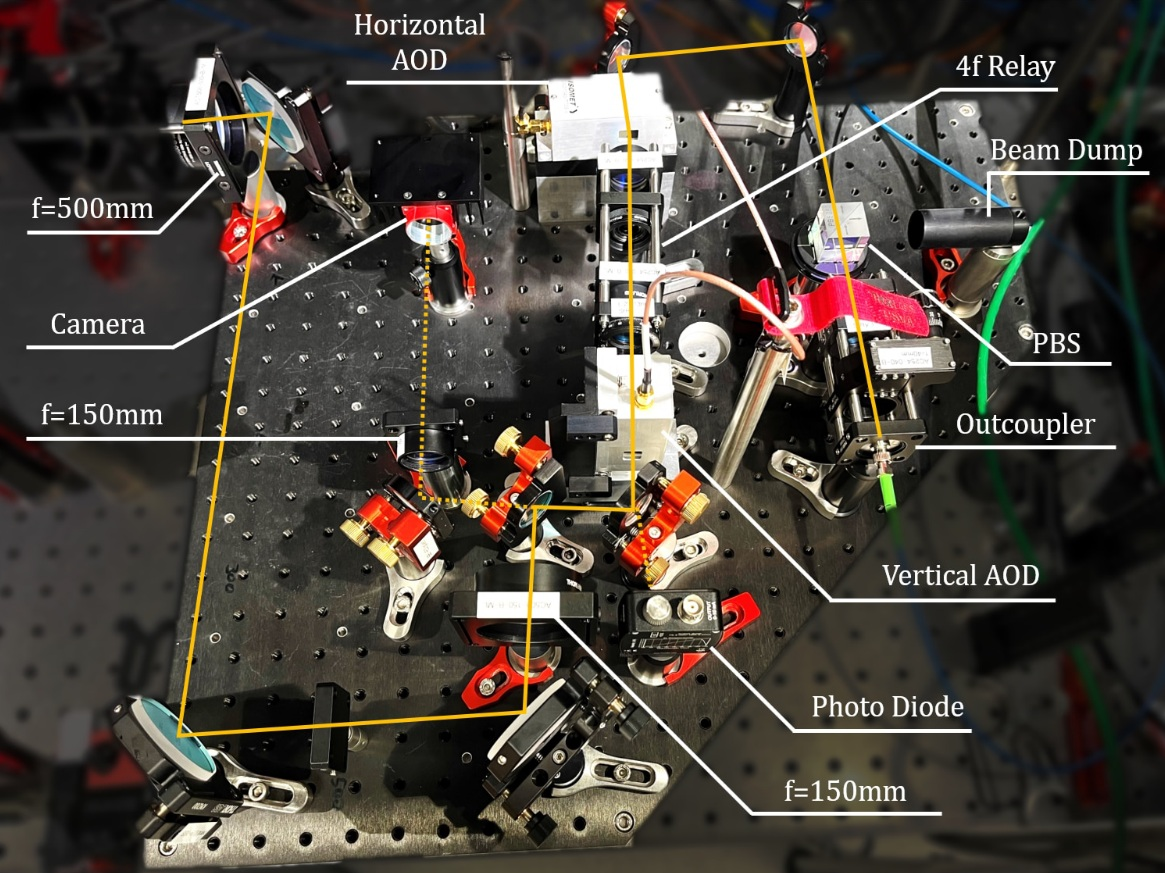
\includegraphics[width=0.5\textwidth]{imgs/tw-setup.jpg}
%     \caption{
%     \textbf{Optical setup for 2D tweezer array.} 
%     The beam path (solid orange line) includes two orthogonal AODs, a $4f$ relay, and diagnostic components. Dashed lines indicate monitoring light paths. Taken from \cite{culemann_construction_2024}.
%     }
%     \label{fig:tw-setup}
% \end{figure}


 












% \begin{figure}
%     \centering
%     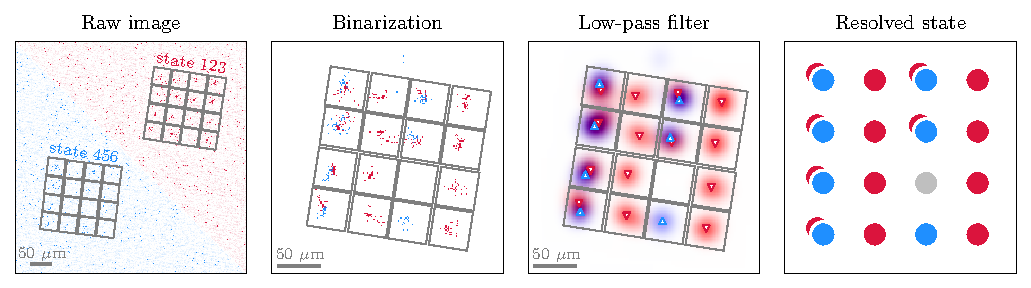
\includegraphics{fig-py/imaging-spin-resolved.pdf}
%     \caption{
%         \textbf{Spin-resolved single-atom imaging.}
%         Spatially separated $\sigma_+$ and $\sigma_-$ fluorescence is imaged onto two distinct regions of the camera. The binarization step identifies photon counts above a threshold, followed by a low-pass filter to extract spatially localized signals. Final spin states are assigned based on relative signal strength in each channel:
%         \raisebox{-1pt}{\scalebox{1.5}{\textcolor{ublue}{\textbullet}}} -- $\ket{1}$, 
%         \raisebox{-1pt}{\scalebox{1.5}{\textcolor{ured}{\textbullet}}} -- $\ket{2}$, 
%         \raisebox{-1pt}{\scalebox{1.5}{\textcolor{uhole}{\textbullet}}} -- no atom.
%     }
%     \label{fig:spin-resolved}
% \end{figure}


% Lorem ipsum dolor sit amet, consectetur adipisicing elit, sed do eiusmod
% tempor incididunt ut labore et dolore magna aliqua. Ut enim ad minim veniam,
% quis nostrud exercitation ullamco laboris nisi ut aliquip ex ea commodo
% consequat. Duis aute irure dolor in reprehenderit in voluptate velit esse
% cillum dolore eu fugiat nulla pariatur. Excepteur sint occaecat cupidatat non
% proident, sunt in culpa qui officia deserunt mollit anim id est laborum.


% \newline
% \phantom{42}
% \newline
% \addletter{100}{c} \phantom{4}
% 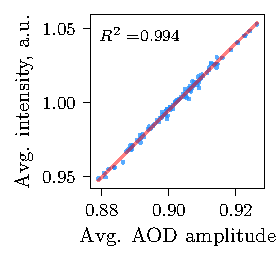
\includegraphics{fig-py/crosstalk-camera-amp.pdf}
% \phantom{4}
% \addletter{100}{d} \phantom{4}
% 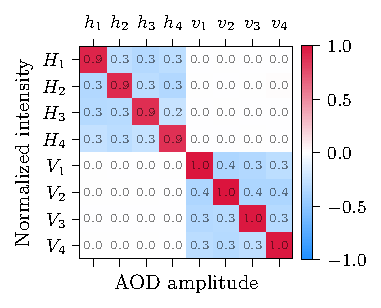
\includegraphics{fig-py/crosstalk-camera.pdf}
% \hfill
% \phantom{4}



--- generating_tw_arr.tex ---
% !TEX root = ../master-thesis.tex

\begin{figure}
    \centering
    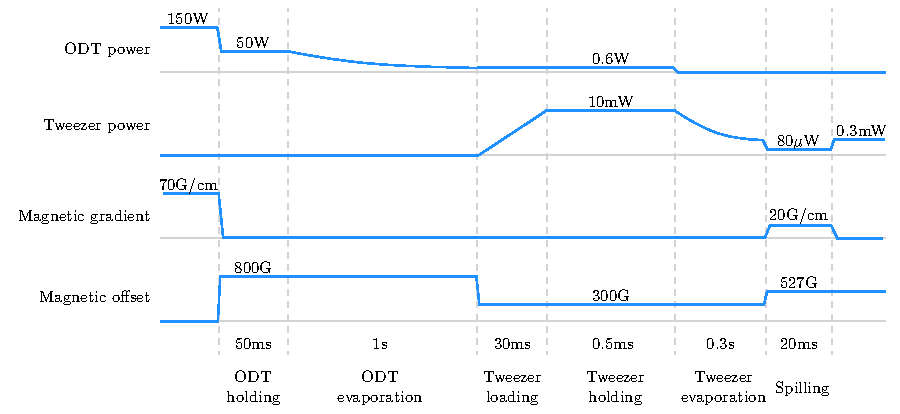
\includegraphics{fig-ai/preparation-seq.pdf}
    \caption{
        \textbf{Experimental sequence for deterministic atom number preparation.} 
        After loading a spin-balanced mixture into a crossed ODT from the MOT, we perform two-stage evaporation in the ODT. The atoms are then transferred into an optical tweezer via an adiabatic ramp. Further evaporation is carried out in the tweezer before executing the spilling procedure. Spilling takes place at 527\,G and a magnetic field gradient of 20\,G/cm to remove atoms above the spill level. The full sequence enables high-fidelity few-body preparation within a sub-2\,s cycle time. A detailed description can be found in~\cite{culemann_construction_2024}.
    }
    \label{fig:preparationseq}
\end{figure}


% \textbf{Acousto Optic Deflector (AOD)}. AOD, как и AOM, состоит из кристалла, который модулируется пьезоэлементом. Проходящие через кристалл фотоны $(\sub{\vc{k}}{in}, \sub{\omega}{in})$ рассеиваются на фононах $(\vc{q}, \Omega)$ via Bragg diffraction. To have higher efficiency we need to satisfy Bragg condition (проверить и добавить источник)
% \begin{equation*}
% 	\sub{n}{sc} q = \sub{k}{in} \sin(\theta),
% \end{equation*}
% \grey{где $\theta$ это угол между $\vc{k}$ и нормалью к $\vc{q}$} \red{(добавить рисунок)}. Внутри AOD находится несколько пьезоэлементов, к которым ведут провода подобранной длины так, чтобы при изменение частоты $\Omega$ направление $\vc{q}$ менялось соответсвующим Bragg condition образом. Это помогает улучшить диффракционную эффективность \grey{(добавить определение или ссылку)} AOD. На выходе полуются $(\sub{\vc{k}}{out}, \sub{\omega}{out}) = (\sub{\vc{k}}{in}+\vc{q}, \sub{\omega}{in} + \Omega)$. 
% Имея набор частот в модулирующем сигнале $(\vc{q}_j, \Omega_j)$ получим на выходе набор лучей
% \begin{equation*}
% 	(p_j, \vc{k}_j, \omega_j) = (F_j(\vc{a}, \sub{\vc{\omega}}{in}), \sub{\vc{k}}{in}+\vc{q}_j, \sub{\omega}{in} + \Omega_j),
% \end{equation*}
% c мощностью в каждом луче на выходе $p_j$. Регулируя вектор амплитуд $\vc{a}$, подающихся в AOD можно контролировать выходную мощность $\vc{p}$. 



\textbf{Beam collimation and polarization.} The tweezer array is formed by delivering light from a fiber outcoupler and collimating it with an $f = 40\,\mathrm{mm}$ achromatic lens mounted on a translation stage for precise control. To ensure efficient diffraction through the acousto-optic deflectors (AODs), horizontal polarization is set using a $\lambda/2$ waveplate and a polarizing beam splitter (PBS). Correct alignment of the PBS is verified by tracking the beam position on a camera before and after insertion.

\textbf{Acousto-optic deflectors and relay imaging.} The array is generated using a pair of orthogonally mounted AODs, each mounted on custom blocks to maintain a common beam height of 100\,mm. The beam is guided into the first AOD using two mirrors, and its alignment is optimized to maximize both transmission and diffraction efficiency (typically exceeding 90\% at 65\,MHz). The two AODs are connected via a 4f relay built from achromatic lenses in a 30\,mm cage system. Precise positioning is achieved by aligning the relay externally using collimated light and checking for minimal wavefront distortion on a shear plate. An iris at the Fourier plane of the relay filters out the zeroth diffraction order.

\textbf{Telescope and beam expansion.} After the second AOD, the beam is expanded using a telescope consisting of $f = 150\,\mathrm{mm}$ and $f = 500\,\mathrm{mm}$ lenses. The alignment ensures that the beam is collimated and centered on both lenses. The position of the second lens is mechanically fixed, while the telescope length is adjusted via mirror positions to achieve good collimation, verified with a shear plate. The zeroth-order beam after the second AOD is blocked at the intermediate focus.

\textbf{Monitoring and power balancing.} A flip mirror is installed in the beam path to optionally redirect the light into a monitoring camera without disturbing the main optical alignment. This enables fast access to the tweezer array profile during alignment or balancing procedures.

We avoid using a back-side polished mirror for beam sampling in front of the camera. Although commonly employed for its simplicity, such mirrors introduce (\red{? add measured data: october 2024}) spatially varying interference fringes due to reflections from different internal surfaces of the substrate. These fringes distort the measured intensity distribution, especially for rays entering the camera at different angles and positions. This effect becomes critical when calibrating the response of the AODs, as it leads to systematic errors in measured beam uniformity. Instead, we sample the beam with a removable flip mirror that fully redirects the beam, ensuring an undistorted and angle-independent intensity profile at the camera plane.


--- imaging-conclusion.tex ---
% !TEX root = ../master-thesis.tex

This chapter has detailed the implementation of a spin-resolved free-space imaging system for ${}^6$Li atoms in an optical tweezer array. The approach is tailored to fast-cycle experiments and leverages the intrinsic spacing of the array to bypass the need for sub-micron spatial resolution.

The free-space fluorescence method was motivated both conceptually and practically, with an emphasis on momentum-space dynamics during imaging. Theoretical considerations based on the SSH model support the use of alternating beam sequences to reduce spatial diffusion, thereby improving localization fidelity.

The optical setup includes two independent laser beams driving stretched-state cycling transitions, with modulation handled via AOMs and synchronized control electronics. A distribution board was constructed to combine and route the beams, ensuring symmetric delivery to the atoms.

The image analysis pipeline applies binarization and spatial filtering to extract single-atom signals from low-flux data. The use of fixed array geometry enables simplified region-of-interest (ROI) analysis and improves classification reliability. All components of the processing chain are implemented in a parallelized, vectorized framework to support high-throughput acquisition.

Spin information is extracted by mapping fluorescence from $\sigma^+$ and $\sigma^-$ transitions to distinct regions on the camera. A per-site classification algorithm assigns spin states based on signal strengths in these regions. Validation against calibrated single-atom counted experiments yields a classification accuracy of approximately 99\% under typical experimental conditions.

These techniques constitute a fast and reliable imaging solution suitable for experiments requiring spin-resolved readout, and are readily extensible to future array sizes and imaging geometries.


--- imaging-flip.tex ---
% !TEX root = ../master-thesis.tex



\begin{figure}
    \centering
    \addletter{105}{a}
    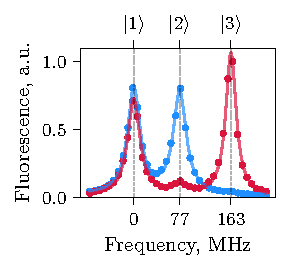
\includegraphics{fig-py/spin-flip-1.pdf}  \phantom{4}
    \addletter{105}{b}
    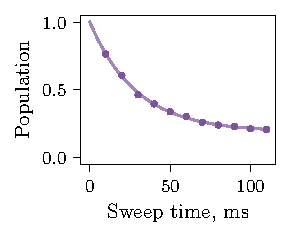
\includegraphics{fig-py/spin-flip-2.pdf}  \phantom{4}
    \addletter{105}{c}
    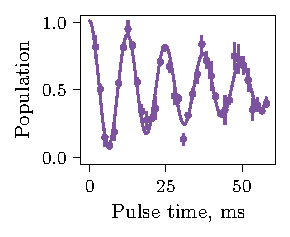
\includegraphics{fig-py/spin-flip-3.pdf}  \phantom{4}
    \caption{
        \textbf{Characterization of spin manipulation protocols.}
        (a) Fluorescence signal measured in the ODT before (blue) and after (red) applying a Landau-Zener sweep between states $\ket{2}$ and $\ket{3}$, showing population transfer to the target state. 
        (b) Final population in $\ket{2}$ as a function of sweep duration, consistent with the Landau-Zener model. 
        (c) Rabi oscillations observed when applying resonant RF $\pi$-pulse between states $\ket{2}$ and $\ket{3}$, demonstrating coherent control of the spin transition. \red{(upd with 17.12.2024)}
    }
    \label{fig:spin-flip}
\end{figure}


\textbf{Introduction and motivation.}
Manipulating the internal spin state of ultracold atoms is an essential element in quantum simulation experiments, particularly for us in context of deterministic state preparation and spin-resolved imaging.
Two widely employed methods for achieving controlled spin transitions in ultracold atomic systems are the Landau-Zener transition and coherent resonant $\pi$-pulse. The Landau-Zener approach involves adiabatically sweeping either the frequency of a driving field or the magnitude of a magnetic field across a spin-resonance. It has been widely applied due to its inherent robustness against small deviations in experimental parameters such as magnetic field fluctuations and frequency drifts. In contrast, the $\pi$-pulse method achieves spin flips by applying a resonant electromagnetic field pulse of precise duration, determined by the corresponding Rabi frequency. Although $\pi$-pulses offer considerably faster spin-flip operations, their fidelity is strongly sensitive to precise calibration of pulse duration, intensity, and frequency detuning, making them more susceptible to experimental noise and parameter instabilities.

Within the context of the current experiment, spin manipulation techniques serve two primary functions. Firstly, flipping atomic spins to stretched states enhances the efficiency of spin-resolved fluorescence imaging. Secondly, selective spin flips are integral to preparation protocols such as spin-selective spilling, allowing controlled removal of atoms in specific spin states. While the Landau-Zener method provided a practical starting point during initial setup stages (mainly due to its robustness against parameter variations) the progression toward faster experimental cycles motivated a transition towards using resonant $\pi$-pulses.

In the following paragraphs, the theoretical foundations of both Landau-Zener and $\pi$-pulse spin manipulation methods are described in detail. A comparative analysis then outlines their respective advantages and limitations in the presence of parameter noise, ultimately justifying the preferred choice adopted in this work.

\textbf{Landau-Zener transition.}
The Landau-Zener (LZ) transition \cite{landau_zur_1932,zener_non-adiabatic_1997} describes the non-adiabatic transition between two quantum states when the energy separation between these states is varied linearly in time. The Hamiltonian governing the dynamics of a two-level system undergoing such a process is expressed as:
\begin{equation}
H_{\text{LZ}}(t) = \frac{\hbar}{2}
\begin{pmatrix}
\Delta(t) & \Omega \
\Omega & -\Delta(t)
\end{pmatrix},
\label{eq:LZ_Hamiltonian}
\end{equation}
where $\Delta(t)$ represents the instantaneous detuning between the system resonance and the external driving field, and $\Omega$ denotes the coupling strength (Rabi frequency) between the two states. Typically, the detuning is varied linearly as $\Delta(t) = \alpha t$, with $\alpha$ defined as the rate of change of detuning.

The transition probability $P_{\text{LZ}}$, derived analytically under the assumption of a linear sweep and constant coupling, is given by the Landau-Zener formula:
\begin{equation}
P_{\text{LZ}} = 1 - \exp\left(-\frac{\pi \Omega^2}{2\alpha}\right).
\label{eq:LZ_probability}
\end{equation}
This probability explicitly depends on the ratio of the squared coupling strength $\Omega^2$ to the detuning sweep rate $\alpha$. For slow sweeps ($\alpha \ll \Omega^2$), the system achieves near-complete transitions ($P_{\text{LZ}}\rightarrow1$), whereas faster sweeps reduce the fidelity (see Fig.~\ref{fig:spin-flip}b).

An important experimental advantage of the Landau-Zener method is its robustness against fluctuations in experimental parameters, such as variations in the magnetic field or the driving frequency. Small deviations in magnetic field gradients or frequency drifts typically have minimal impact on transition fidelity due to the exponential character of Eq.~\eqref{eq:LZ_probability}. This robustness is particularly valuable in experiments where shot-to-shot variations in magnetic fields are inevitable.

Despite its robustness, the Landau-Zener transition requires relatively long timescales ($t_{\text{LZ}} \gg 1/\Omega$) to achieve high transition fidelities, which can slow down experimental cycles and increase exposure to decoherence processes.

\textbf{Rabi $\pi$-pulse.}
An alternative technique for coherent spin manipulation is the resonant Rabi oscillation method, commonly known as the $\pi$-pulse approach. This method exploits coherent driving of the transition between two spin states at constant resonance, enabling deterministic and rapid population transfer.

The dynamics under resonant excitation are described by the Hamiltonian in Eq.~\eqref{eq:LZ_Hamiltonian} with a constant detuning $\Delta=\text{const}$. By applying a resonant driving field ($\Delta=0$) for the duration $t_\pi = \pi/\Omega$, the system achieves complete inversion of the spin populations, thus realizing an ideal spin-flip operation between states $\ket{1}$ and $\ket{2}$.

The primary advantage of the $\pi$-pulse technique is its speed: the required pulse duration is significantly shorter than that for Landau-Zener sweeps ($t_\pi \ll t_{\text{LZ}}$), as evidenced by rapid Rabi oscillations in Fig.~\ref{fig:spin-flip}c. However, the fidelity of $\pi$-pulse transitions is highly sensitive to deviations from the exact resonance condition ($\delta \neq 0$), as well as inaccuracies in pulse duration and field amplitude. This sensitivity is captured analytically by the generalized Rabi oscillation formula:
\begin{equation}
P_{\pi} = \frac{\Omega^2}{\Omega^2+\delta^2}\sin^2\left(\frac{\sqrt{\Omega^2+\delta^2}}{2}t_{\pi}\right).
\label{eq:pi_fidelity}
\end{equation}

Shot-to-shot fluctuations, especially those in the magnetic field, directly translate into variations in resonance conditions and consequently introduce systematic and random errors in spin-flip fidelity. As a result, consistently high fidelity using $\pi$-pulses necessitates stringent experimental stabilization of magnetic fields, pulse timing, and amplitude calibration.


\textbf{In this experiment.}
In the present experiment, spin-state populations are routinely measured by scanning the laser frequency while simultaneously recording the fluorescence signal of atoms either confined in the ODT or directly in optical tweezers. Figure~\ref{fig:spin-flip}a demonstrates a typical example, showing clear fluorescence peaks corresponding to distinct spin states. Such spectral scans provide a reliable quantitative method for assessing the efficiency of spin-state transitions.

\red{Initially, spin manipulation in this experiment relied primarily on Landau-Zener sweeps. Operating at moderate coupling strengths ($\Omega \sim 1~\text{kHz}$), transition fidelities around 95\% were achieved. Subsequent technical improvements in the RF and MW antenna designs allowed increasing the effective coupling strength up to approximately 10~kHz. Employing $\pi$-pulses at this higher coupling strength consistently yielded fidelities of 99\% or greater, primarily due to reduced sensitivity to decoherence over shorter timescales.}
In conclusion, while Landau-Zener sweeps provided a robust and convenient method for spin-state manipulation during initial setup phases, the improvements in RF/MW coupling strengths ultimately favored the adoption of faster and more efficient $\pi$-pulse protocols.

--- imaging-motivation.tex ---
% !TEX root = ../master-thesis.tex

\textbf{Role of imaging in fast-cycle experiments.}  
In high-repetition quantum simulation experiments with ${}^6$Li, fast, minimally disruptive, and high-fidelity single-atom detection is essential. Free-space imaging~\cite{bergschneider_spin-resolved_2018,su_fast_2025} offers a simple and efficient alternative to traditional Raman-based fluorescence imaging. In this method, atoms are released from their traps and illuminated with resonant light. Fluorescence is collected without requiring additional cooling or deep pinning potentials. The short exposure time, typically around $10~\mu$s, allows for much higher experimental repetition rates compared to standard approaches based on quantum gas microscopes.

\textbf{Free-space imaging for ${}^6$Li.}  
Although ${}^6$Li is a light atom and experiences relatively large momentum recoil during scattering, its broad D2 transition at $\lambda = 671$~nm allows for rapid photon emission. The typical recoil velocity is given by $v_\mathrm{rec} = {h}/{m \lambda}$, where $m$ is the atomic mass of ${}^6$Li and $\lambda$ is the wavelength of the imaging light. As the atom scatters photons at a rate $\Gamma$, each with random emission direction, it undergoes a random walk in momentum space. This results in spatial diffusion during the imaging pulse. The root-mean-square width of this random walk is approximately \cite{kruip_design_2024} (in the flashing regime)
\begin{equation}
	\sigma_\mathrm{rw} = \tfrac{1}{3} v_\mathrm{rec} \Gamma^{1/2} t^{3/2},
	\label{eq:sigmarw}
\end{equation}
where $t$ is the total exposure time. For a fixed number of scattered photons $N_\mathrm{ph}$, we can express $t = N_\mathrm{ph} / \Gamma$, yielding
\begin{equation}
	\sigma_\mathrm{rw} = \tfrac{1}{3} v_\mathrm{rec} \Gamma^{-1} N_\mathrm{ph}^{3/2}.
\end{equation}

This scaling highlights the trade-off between collecting more fluorescence photons and maintaining spatial resolution. In our system, with $N_\mathrm{ph} \sim 300$, the resulting diffusion is on the scale of $10~\mu$m.
% making single-atom detection feasible 


\begin{figure}[htb]
    \centering
    \addletter{140}{a}
    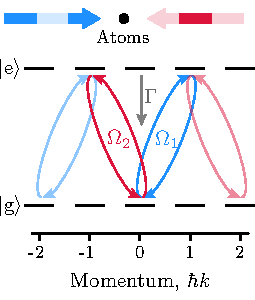
\includegraphics{fig-ai/ssh-scheme.pdf}
    \hfill
    \addletter{140}{b}
    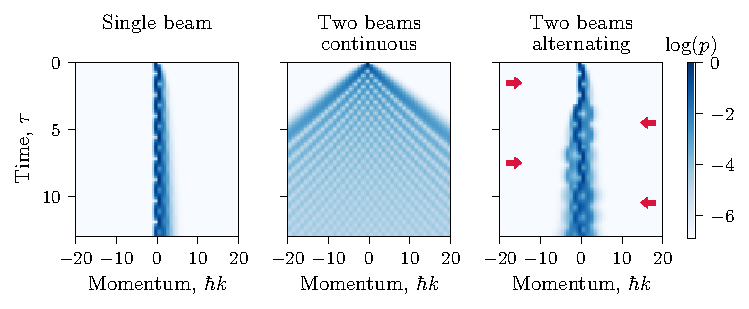
\includegraphics{fig-py/ssh-model.pdf}
    \caption{
        \textbf{Momentum-space dynamics in the SSH model}. 
        a) Atoms undergo momentum-changing transitions via couplings $\Omega_1$ and $\Omega_2$, realizing a SSH-like quantum walk.
        b) Momentum distributions over time for different beam configurations: single beam (left) shows small shift; two continuous beams (middle) result in fast spreading; alternating beams (right) suppress spread.
    }
    \label{fig:sshmodel}
\end{figure}


\textbf{Connection to the SSH model.}  
The scattering dynamics of a freely moving atom illuminated by resonant counter-propagating beams can be understood as a momentum-space quantum walk. This process maps onto the Su-Schrieffer-Heeger (SSH) model:
\begin{equation*}
	H = t_1 \sum_n \ket{n,B}\bra{n,A} + t_2 \sum_n \ket{n+1,A}\bra{n,B} + \text{h.c.}
\end{equation*}
In the atomic case, the model takes the form:
\begin{equation*}
	H = \frac{\Omega_1}{2} \sum_p \ket{p,g}\bra{p+1,e} + \frac{\Omega_2}{2} \sum_p \ket{p-1,e}\bra{p,g} + \text{h.c.}
\end{equation*}
Here, $\Omega_1$ and $\Omega_2$ correspond to the Rabi frequencies of the two beams. When both beams are on simultaneously, the atom undergoes coherent transitions between distant momentum states. This leads to rapid delocalization in space. The evolution can be simulated by solving a Lindblad master equation,
\begin{equation*}
	i \hbar \partial_t \rho = [H(t), \rho] + \mathcal{L}[\rho],
\end{equation*}
with $\mathcal{L}$ describing spontaneous emission. These simulations show that applying the two beams alternately—rather than simultaneously—dramatically suppresses spatial diffusion and improves imaging fidelity (Fig.~\ref{fig:sshmodel}).

\textbf{Spin-resolved imaging with stretched states.}  
To perform spin-resolved detection with high signal strength, atoms are transferred into stretched states $\ket{3}$ and $\ket{6}$ before imaging. These states are nearly pure $m_J = \pm 1/2, m_I = \mp 1$ at high magnetic fields and couple strongly to $\sigma^\pm$ polarized light. Unlike the commonly used $\ket{1}$ and $\ket{2}$ states, which have small admixtures that allow decay into dark states, $\ket{3}$ and $\ket{6}$ support nearly closed cycling transitions. As a result, atoms in these states scatter significantly more photons, often nearly twice as many, which greatly improves detection efficiency.

To distinguish the two spin states during a single imaging pulse, their respective fluorescence is spatially separated on the camera. This is achieved by using a polarizing beam splitter (PBS) after the objective, which directs $\sigma^+$ and $\sigma^-$ components to different regions of the detector (see Fig.~\ref{fig:spin-resolved}). By analyzing the relative photon counts in these regions, one can assign the spin state of each detected atom with high fidelity, as described in Sec.~\ref{subsec:imaging-spin}.

\textbf{Overview of this section.}  
The following subsections describe the complete implementation of spin-resolved free-space imaging in our experiment. Section~\ref{subsec:imaging-setup} details the optical setup built and aligned during this work. Section~\ref{subsec:imaging-processing} explains the image analysis pipeline, which was developed as part of this thesis. Finally, Section~\ref{subsec:imaging-spin} presents the spin-state discrimination method and evaluates its fidelity using experimental calibration data. Together, these elements form a robust and fast readout protocol for our ${}^6$Li tweezer-based simulator.



% Мы работаем с Li6, делаем fast cycle quantum simulator, так что free space imaging предложенный в \cite{bergschneider_spin-resolved_2018} является для нас отличным кандидатом: быстро, просто в реализации (за исключением MWM), spin-resolved. Да, из-за размытия, сам по себе имеет разрешающую способность около 10$\mu$m для Li6 (в контексте нашего эксперимента), так что lattice single-site resolved imaging требует дополнительно использования Matter Wave Magnifier, но мы и будем его использовать а численное моделирование можно найти дальше у меня в дипломе. Но для нас на данном этапе этот метод отлично работал для фотографирования атомов в tweezers, так как можем сами расположить на достаточно для single site imaging. 


% Тут пригодятся эти картинки:


% \begin{figure}[h]
%     \centering
%     \addletter{200}{a}
%     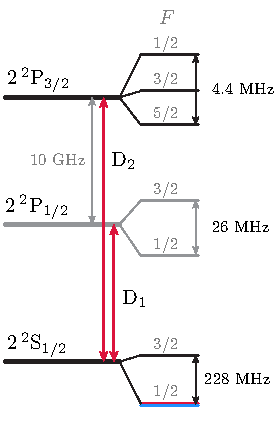
\includegraphics{fig-ai/li-levels-base.pdf}
%     \hspace{1cm}
%     \addletter{200}{b}
%     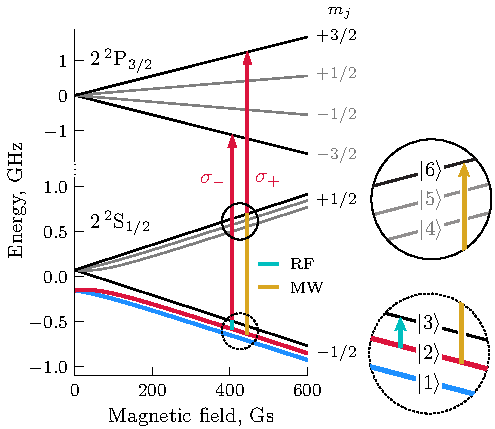
\includegraphics{fig-ai/li6-zeeman-broken-ai.pdf}
%     \caption{
%         \textbf{${}^6$Li energy levels}. 
%         a) Level diagram of the ground and excited states of ${}^6$Li \cite{gehm_preparation_2003}, including the D1 and D2 transitions around $\lambda = 671$~nm. 
%         b) Zeeman splitting of the hyperfine levels of the $2\, {}^2\mathrm{S}_{1/2}$ and $2\, {}^2\mathrm{P}_{2/2}$ in ${}^6$Li \cite{serwane_deterministic_2011, sibalic_arc_2017}. As different spin states for physics we consider state $\ket{1}$ and $\ket{2}$, but for imaging it is worth to flip them to stretched states $\ket{6}$, $\ket{3}$. Colored lines indicate transitions driven by radiofrequency (RF) and microwave (MW) fields.
%     }
%     \label{fig:li6levels}
% \end{figure}


% \begin{figure}[h]
%     \centering
%     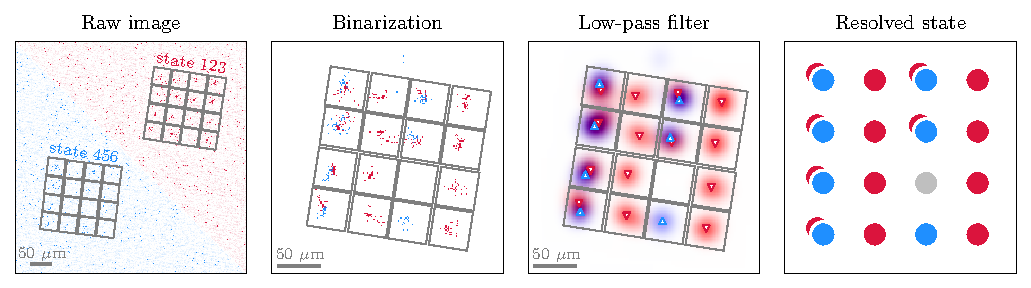
\includegraphics{fig-py/imaging-spin-resolved.pdf}
%     \caption{
%         \textbf{Spin-resolved single-atom imaging.}
%         Spatially separated $\sigma_+$ and $\sigma_-$ fluorescence is imaged onto two distinct regions of the camera. The binarization step identifies photon counts above a threshold, followed by a low-pass filter to extract spatially localized signals. Final spin states are assigned based on relative signal strength in each channel:
%         \raisebox{-1pt}{\scalebox{1.5}{\textcolor{ublue}{\textbullet}}} -- $\ket{1}$, 
%         \raisebox{-1pt}{\scalebox{1.5}{\textcolor{ured}{\textbullet}}} -- $\ket{2}$, 
%         \raisebox{-1pt}{\scalebox{1.5}{\textcolor{uhole}{\textbullet}}} -- no atom.
%     }
%     \label{fig:spin-resolved}
% \end{figure}


% В чем заключался мой вклад? Я реализовал оптическую схему, которая работает на 17 mW мощности одного лазера 671 нм (aka imaging), и выдаёт в каждый из flashing лучей 1 mW мощности (соответствуя в итоге $\sub{s}{sat} \sim 5$). И \red{X} mW другого лазера 671 нм (aka RFA). На схеме примерно 1 mW "imaging laser" идёт на стабилизацию, остальное проходит через контролирующие AOM (для вкл выкл, это Gooch & Housego 3080-120 на 80 MHz x2), beam spliiter (там же лучи RFA и Imaging совмещаются) и разделяются на left and right optical beams (imaging надо делать с двух сторон) и проходят через "flashing" aom (Gooch & Housego 3110-120 на 80 MHz x2), упровляемые через генератор сигналов (Rigol) на который и подаём ступеньки с периодом 1MHz, и потом уже заводятся в оптоволокно. Для повышения эффективности enabling AOM перед ними стоит линза 1000mm (LA1464-B). Два лазера используются, так как для spin resolve imaging нам нужно  работать с двумя переходами, отстоящими на 0.5 GHz. 




% \begin{figure}[h]
%     \centering
%     \addletter{195}{a} \phantom{4}
%     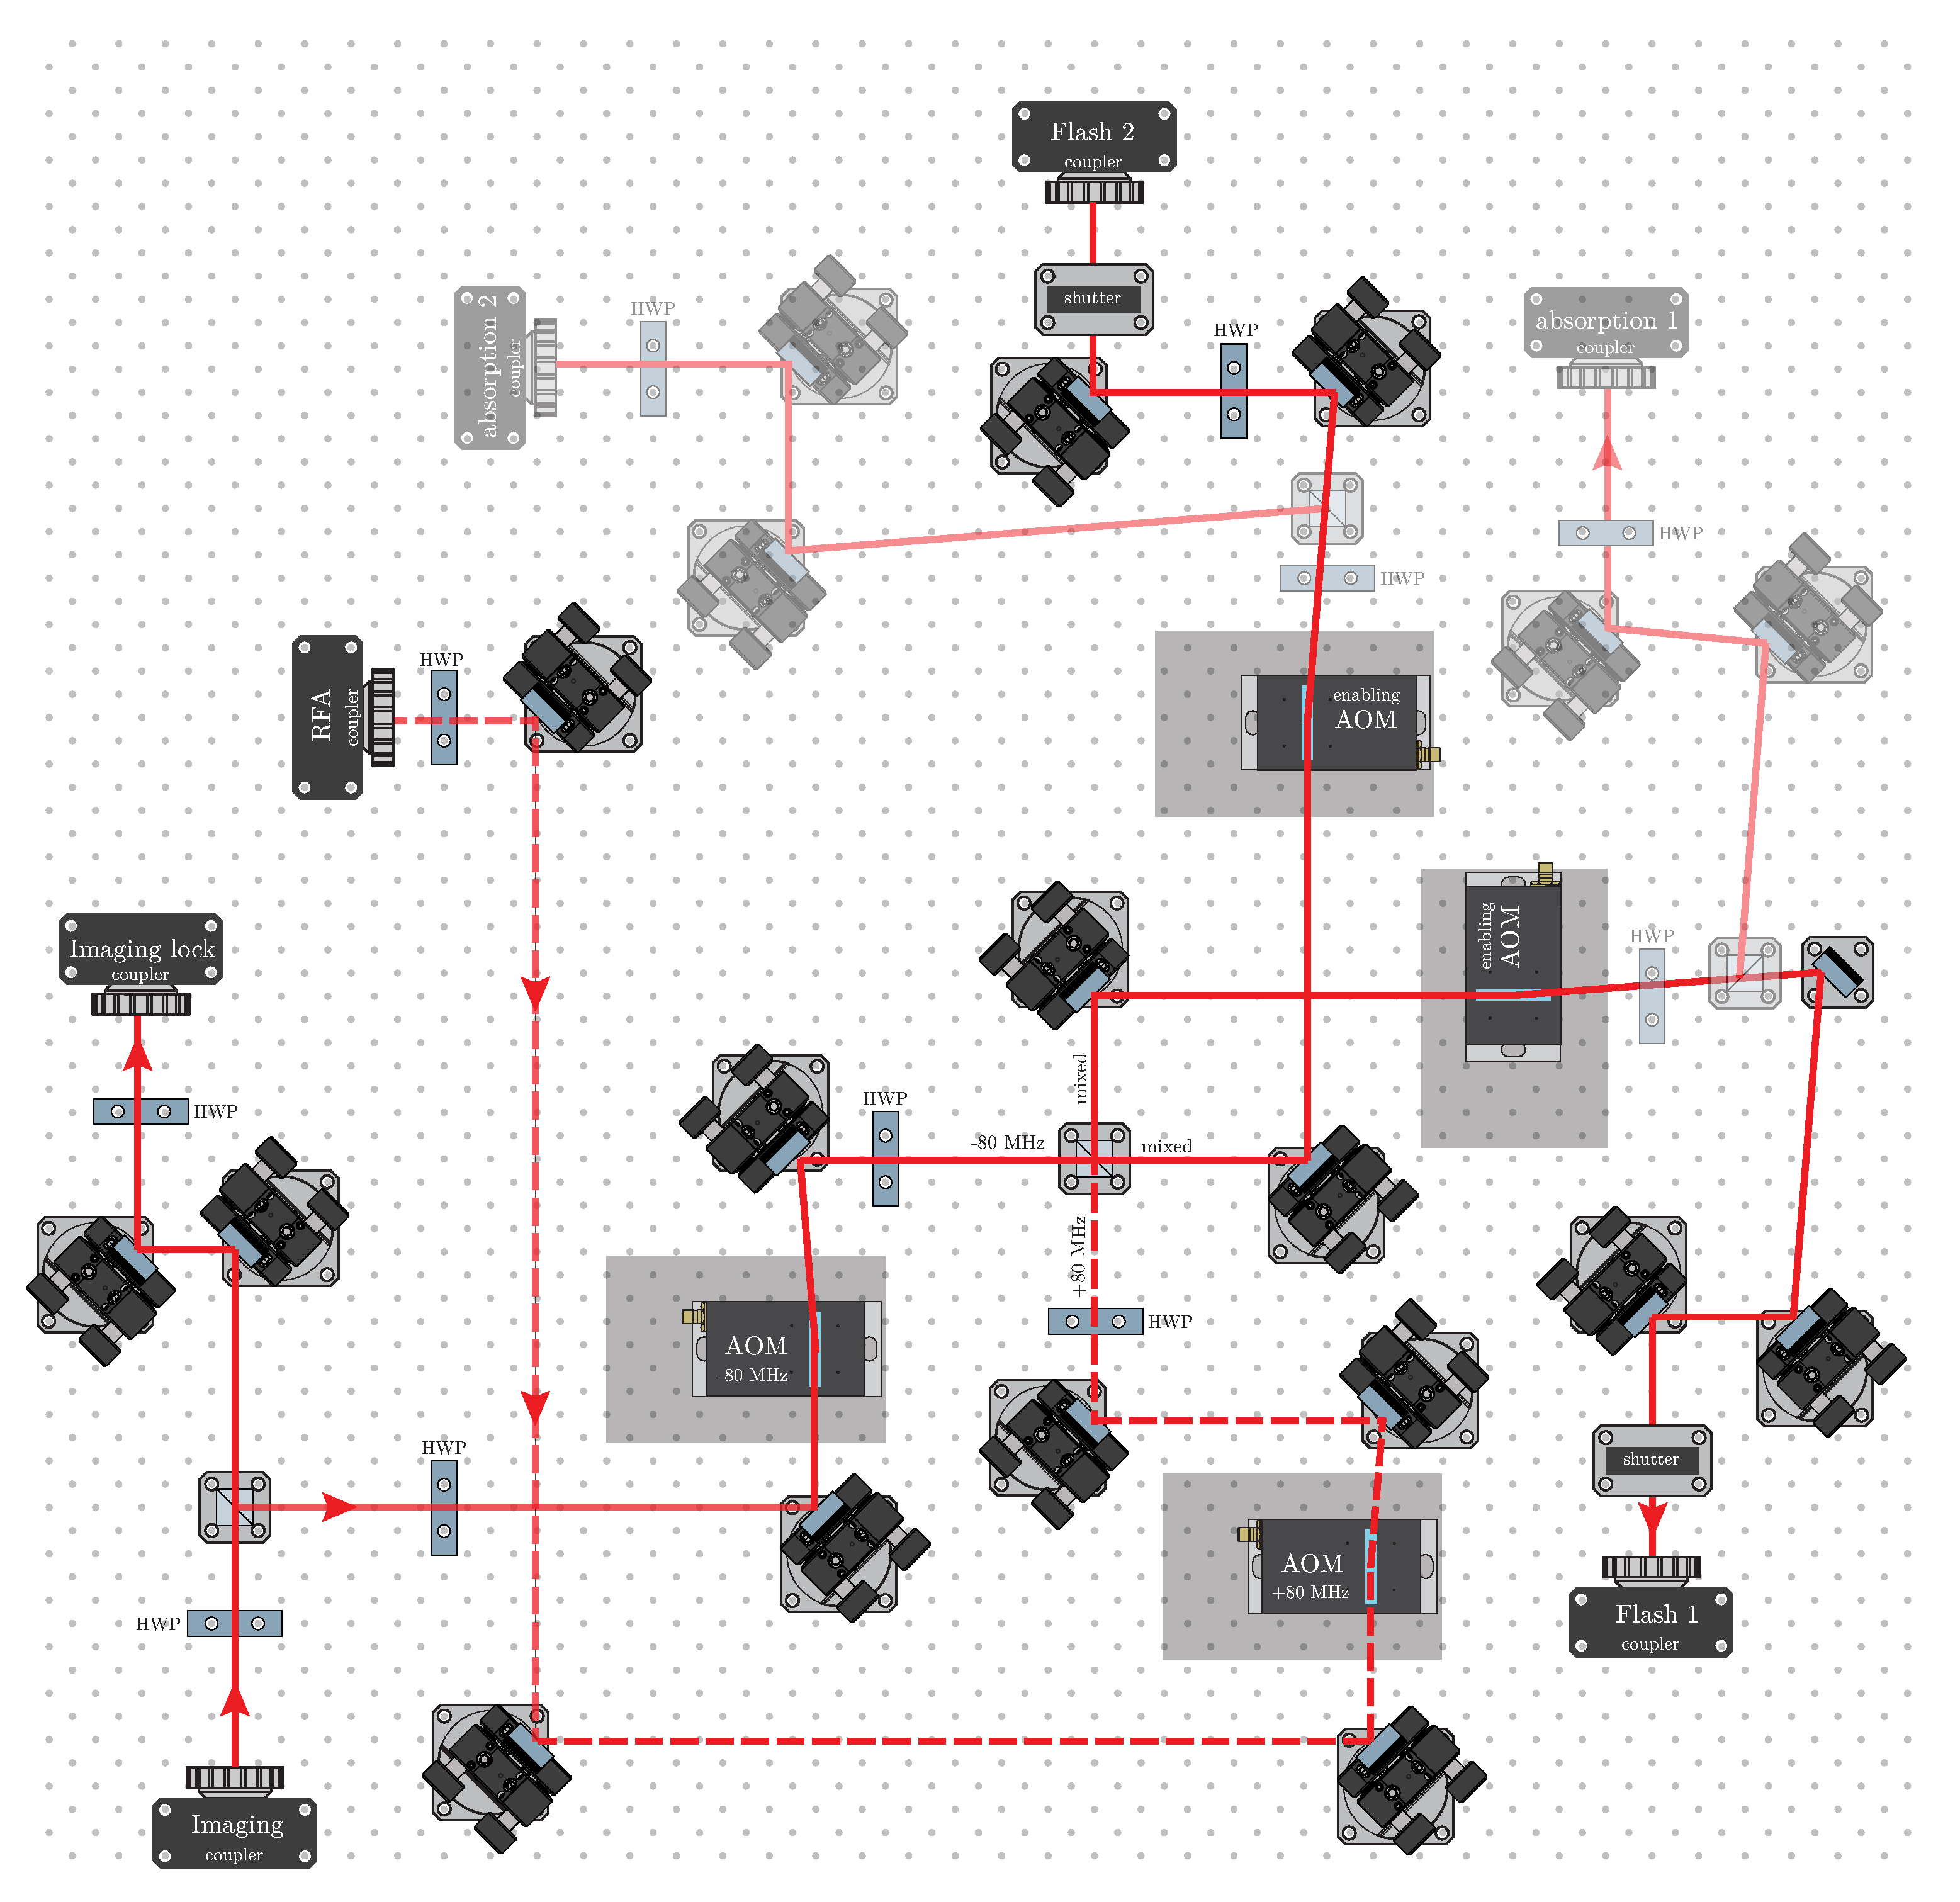
\includegraphics[width=0.4\textwidth]{fig-ai/flashing-distribution-scheme.pdf}
%     \hspace{10 mm} 
%     \addletter{195}{b} \phantom{4}
%     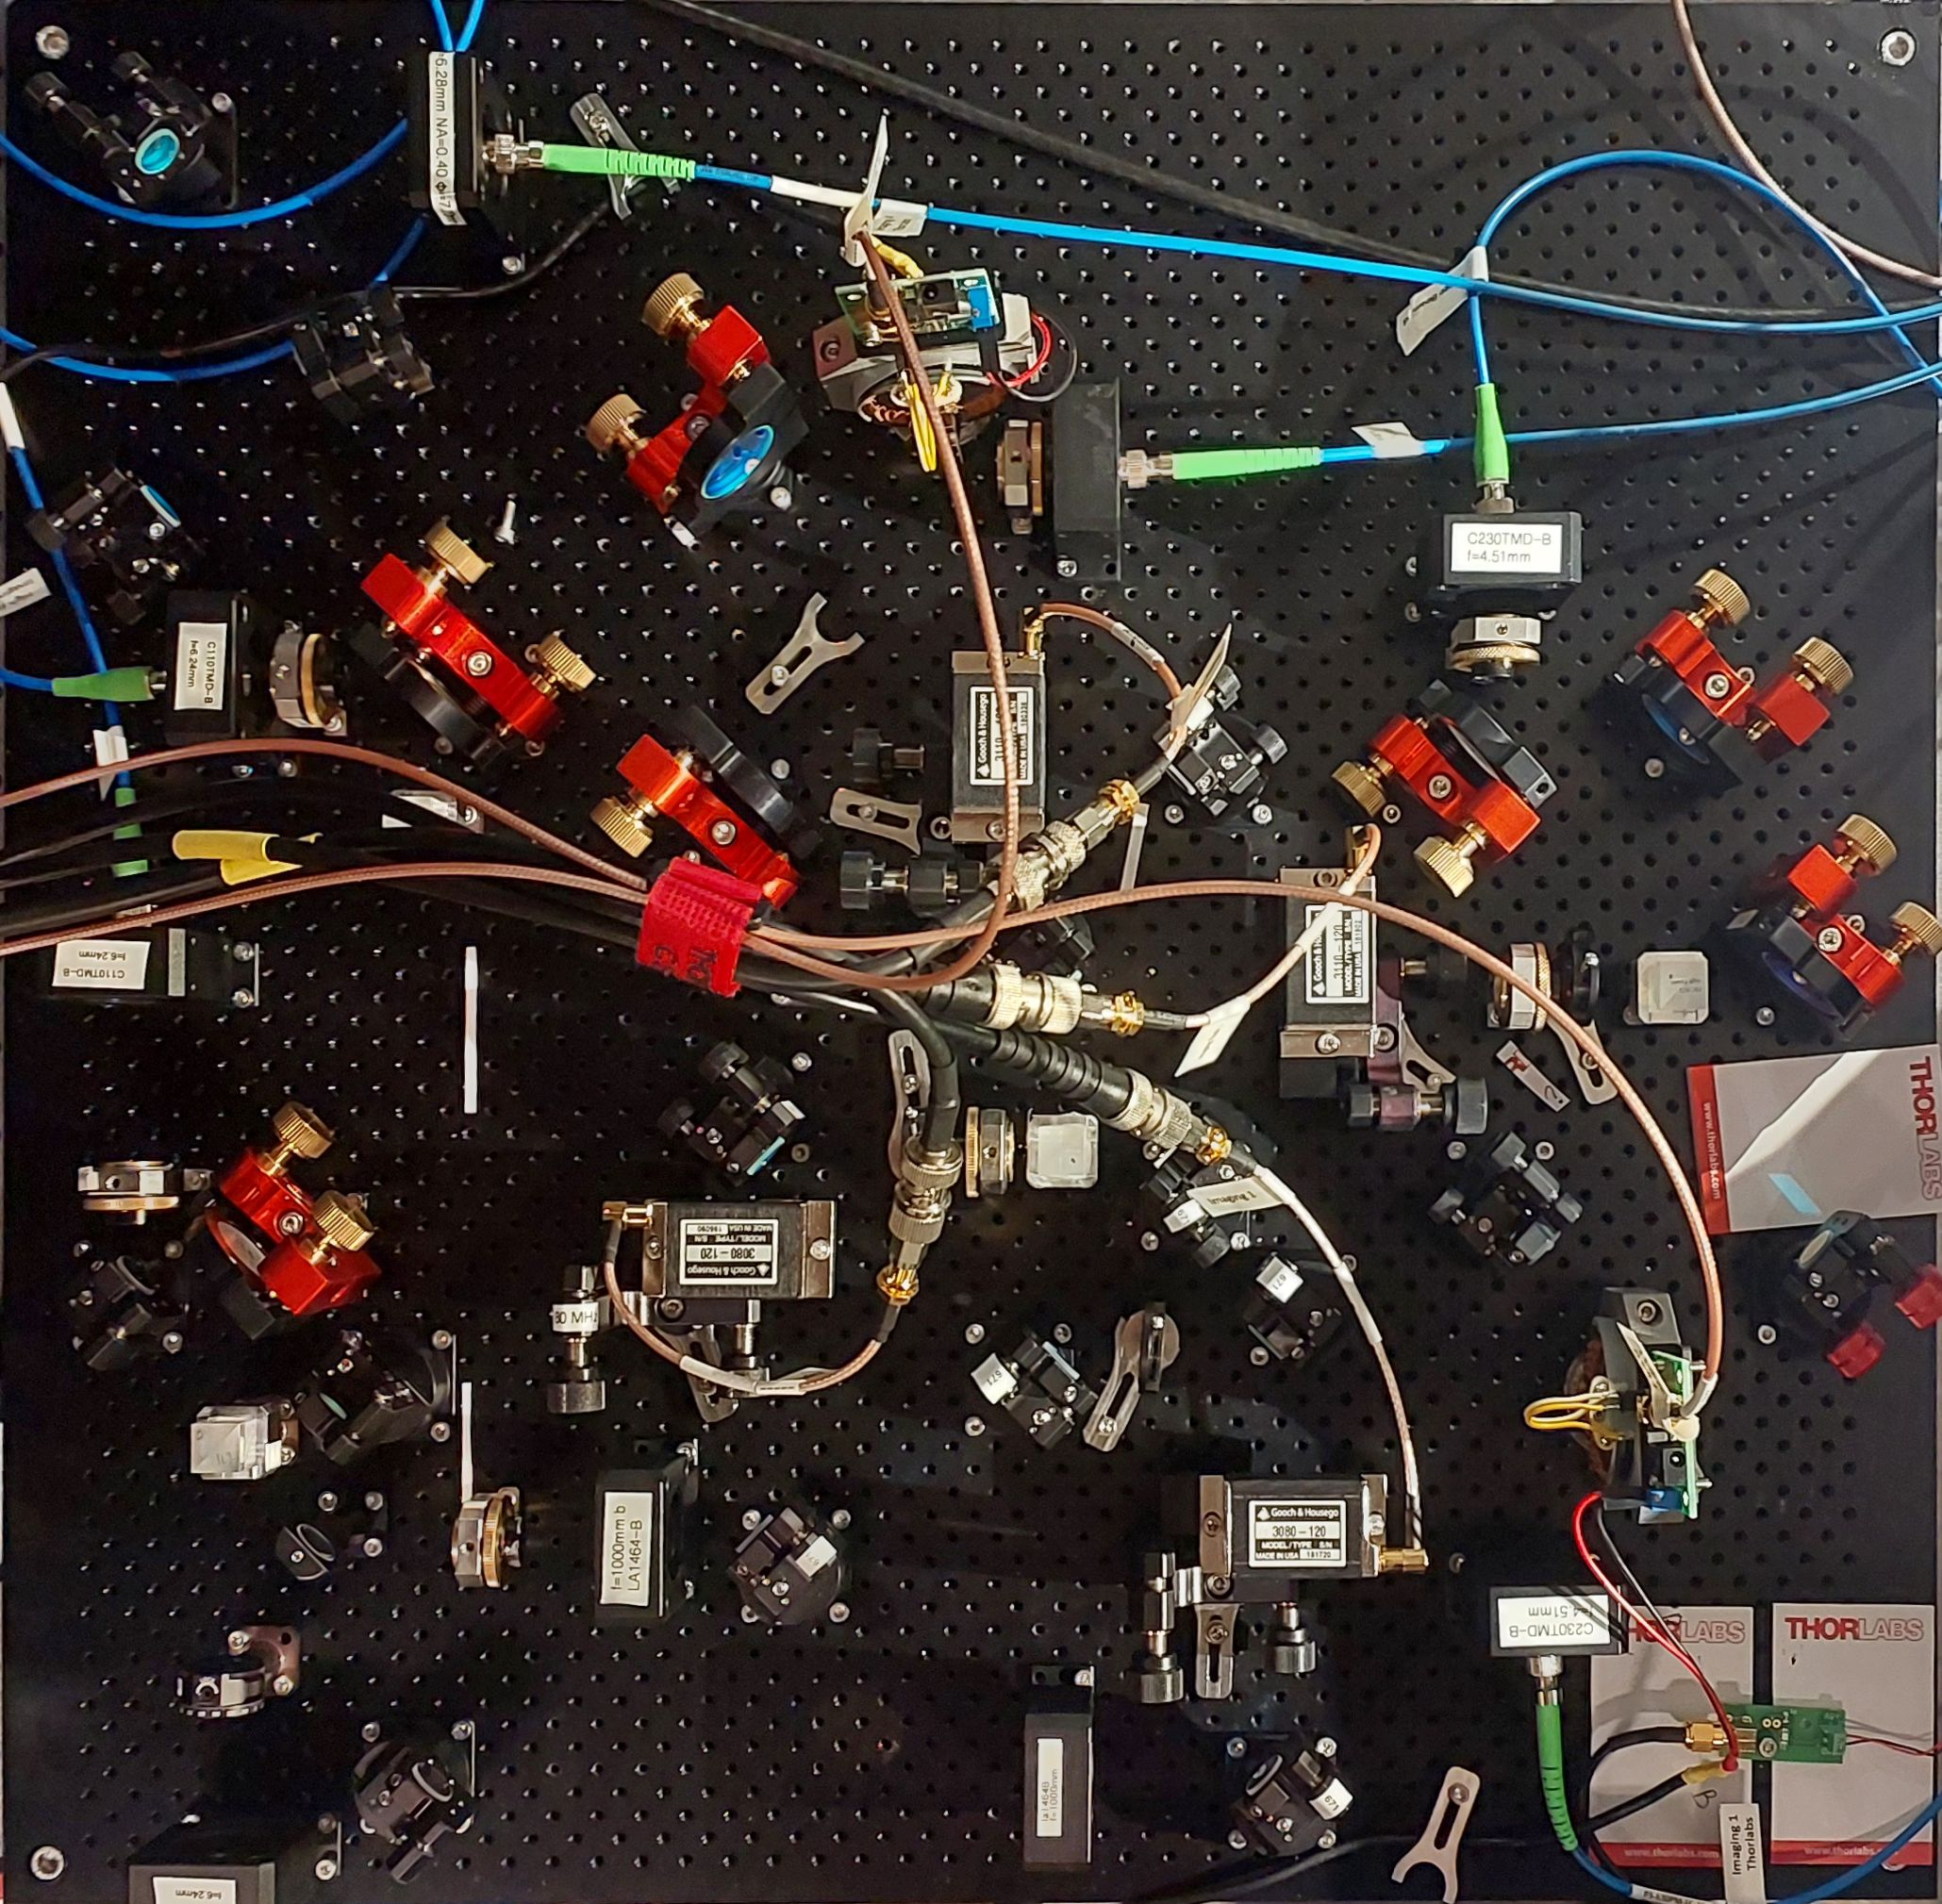
\includegraphics[width=0.4\textwidth]{imgs/flashing-distribution-img.jpg}

%     \addletter{90}{c}
%     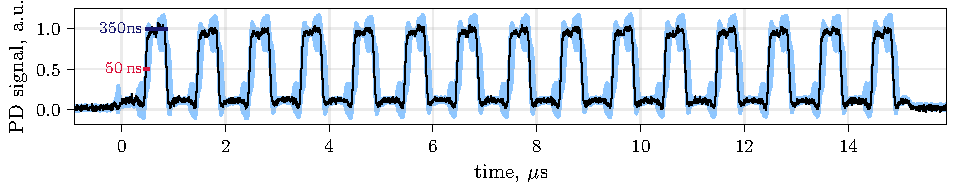
\includegraphics{fig-py/flashing-oscilloscope.pdf}

%     \caption{
%         \textbf{Distribution board for flashing}. 
%         a) Optical layout of the board used to combine and control light for free-space imaging states $\ket{3}$ and $\ket{6}$.
%         b) Experimental implementation.
%         c) PD signal of the flashing measured on an oscilloscope (black -- a single experimental run, blue -- the standard deviation over 20 runs, red -- rise time).
%     }
%     \label{fig:flashing}
% \end{figure}


--- imaging-processing.tex ---
% !TEX root = ../master-thesis.tex


\begin{figure}
    \centering
    \addletter{125}{a}
    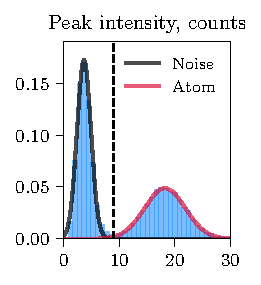
\includegraphics{fig-py/imaging-hist.pdf}
    \hfill
    \addletter{125}{b}
    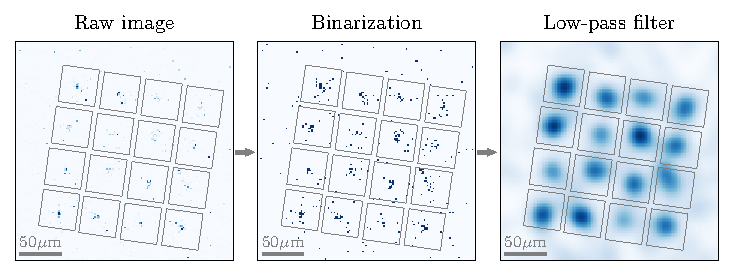
\includegraphics{fig-py/imaging-base.pdf}
    \caption{
        \textbf{Single-atom identification and image processing.}
        a) Histogram of peak intensities extracted from binarized and low-pass filtered images shows a bimodal distribution: the first peak corresponds to camera noise (black), the second corresponds to single atoms (red). The dashed line indicates the threshold used for atom identification.
        b) Image processing pipeline: Raw fluorescence image (left), binarization by intensity thresholding (center), and application of a low-pass filter (right) to reveal spatially localized atomic signals. 
        % \red{Для (a) можно добавить fit, показав что иногда случаются и два атома.}
    }
    \label{fig:imaging}
\end{figure}

\textbf{Camera and detection regime.}  
The imaging system uses a Nüvü HNü512 EMCCD camera, chosen for its high sensitivity and low noise in the few-photon regime. At $\lambda = 671$~nm, the sensor achieves a quantum efficiency (QE) of approximately 94\%~\cite{kruip_design_2024}. The camera is operated in photon counting mode with EM gain up to 5000, enabling single-atom detection from just tens of detected photons. During a typical imaging sequence, each atom emits around 300 photons, of which approximately 30 are detected on the camera after collection and transmission losses.

\textbf{Binarization and filtering pipeline.}  
To mitigate the excess noise factor (ENF) inherent in EM amplification and to suppress clock-induced charges (CICs), we apply a binarization scheme. A fixed threshold (typically $5\sigma_\text{read}$ above the baseline noise) is used to convert raw images into binary maps, where each pixel is marked as "bright" if it exceeds the threshold and "dark" otherwise. This removes ambiguity due to the stochastic gain distribution and allows images to be treated as photon arrival maps.  

To reduce high-frequency noise while preserving localized atomic signals, we apply a Gaussian low-pass filter with a tunable width (typically $\sigma = 7$ px). This smooths the binarized images and helps identify spatially coherent clusters corresponding to single atoms. \red{Optionally, a denoising step based on a circular neighbor-count kernel can be applied after binarization; see Appendix for implementation details.}

\textbf{Atom identification from local maxima.}  
We locate candidate atom positions by searching for local maxima in the filtered images. Since the imaging beam is symmetric and atoms are spatially separated (due to the tweezer geometry), each atom forms a compact signal peak. To distinguish real atoms from CIC-induced noise clusters, we construct a histogram of peak amplitudes and apply a classification threshold based on the bimodal structure (see Fig.~\ref{fig:imaging}). This provides a robust method for single-atom detection within each image.

\textbf{Use of ROI and regular array geometry.}  
During this work, all experiments were performed with a regular tweezer array. This allows us to restrict image analysis to known regions of interest (ROIs) around each expected atom location. This prior knowledge significantly simplifies the classification problem: we identify the atom at a given site as present or absent based on the presence of a peak in the corresponding ROI. This enables more reliable classification than in fully general imaging tasks as in \cite{bergschneider_spin-resolved_2018}.

\textbf{Implementation and contribution.}  
The entire image analysis pipeline (bias correction, binarization, optional denoising, filtering, and classification) was implemented by the author in Python. The resulting code is vectorized and supports batch processing of image sequences. While the core concepts draw from existing methods developed in~\cite{bergschneider_spin-resolved_2018}, the current implementation is adapted to the geometry and noise characteristics of our setup. 
% Notably, the simplification due to known array geometry enables efficient and accurate analysis suitable for high-throughput acquisition.


--- imaging-setup.tex ---
% !TEX root = ../master-thesis.tex


% \red{Здесь схема оптики для подготовки лучей в preparation board и схема лучей и подключения для main board}.

\textbf{Laser configuration and frequency scheme.}  
The imaging system uses two frequency-stabilized diode lasers, each tuned to drive a stretched-state cycling transition in ${}^6$Li: $\ket{3} \rightarrow \ket{3'}$ and $\ket{6} \rightarrow \ket{6'}$. These transitions are addressed independently to enable spin-resolved fluorescence collection. Both lasers are frequency-locked to atomic references \red{(see Appendix for further details on the stabilization scheme)}. The system does not require additional repumping during imaging, as both target states are closed under cycling.


\begin{figure}
    \centering
    \addletter{195}{a} \phantom{4}
    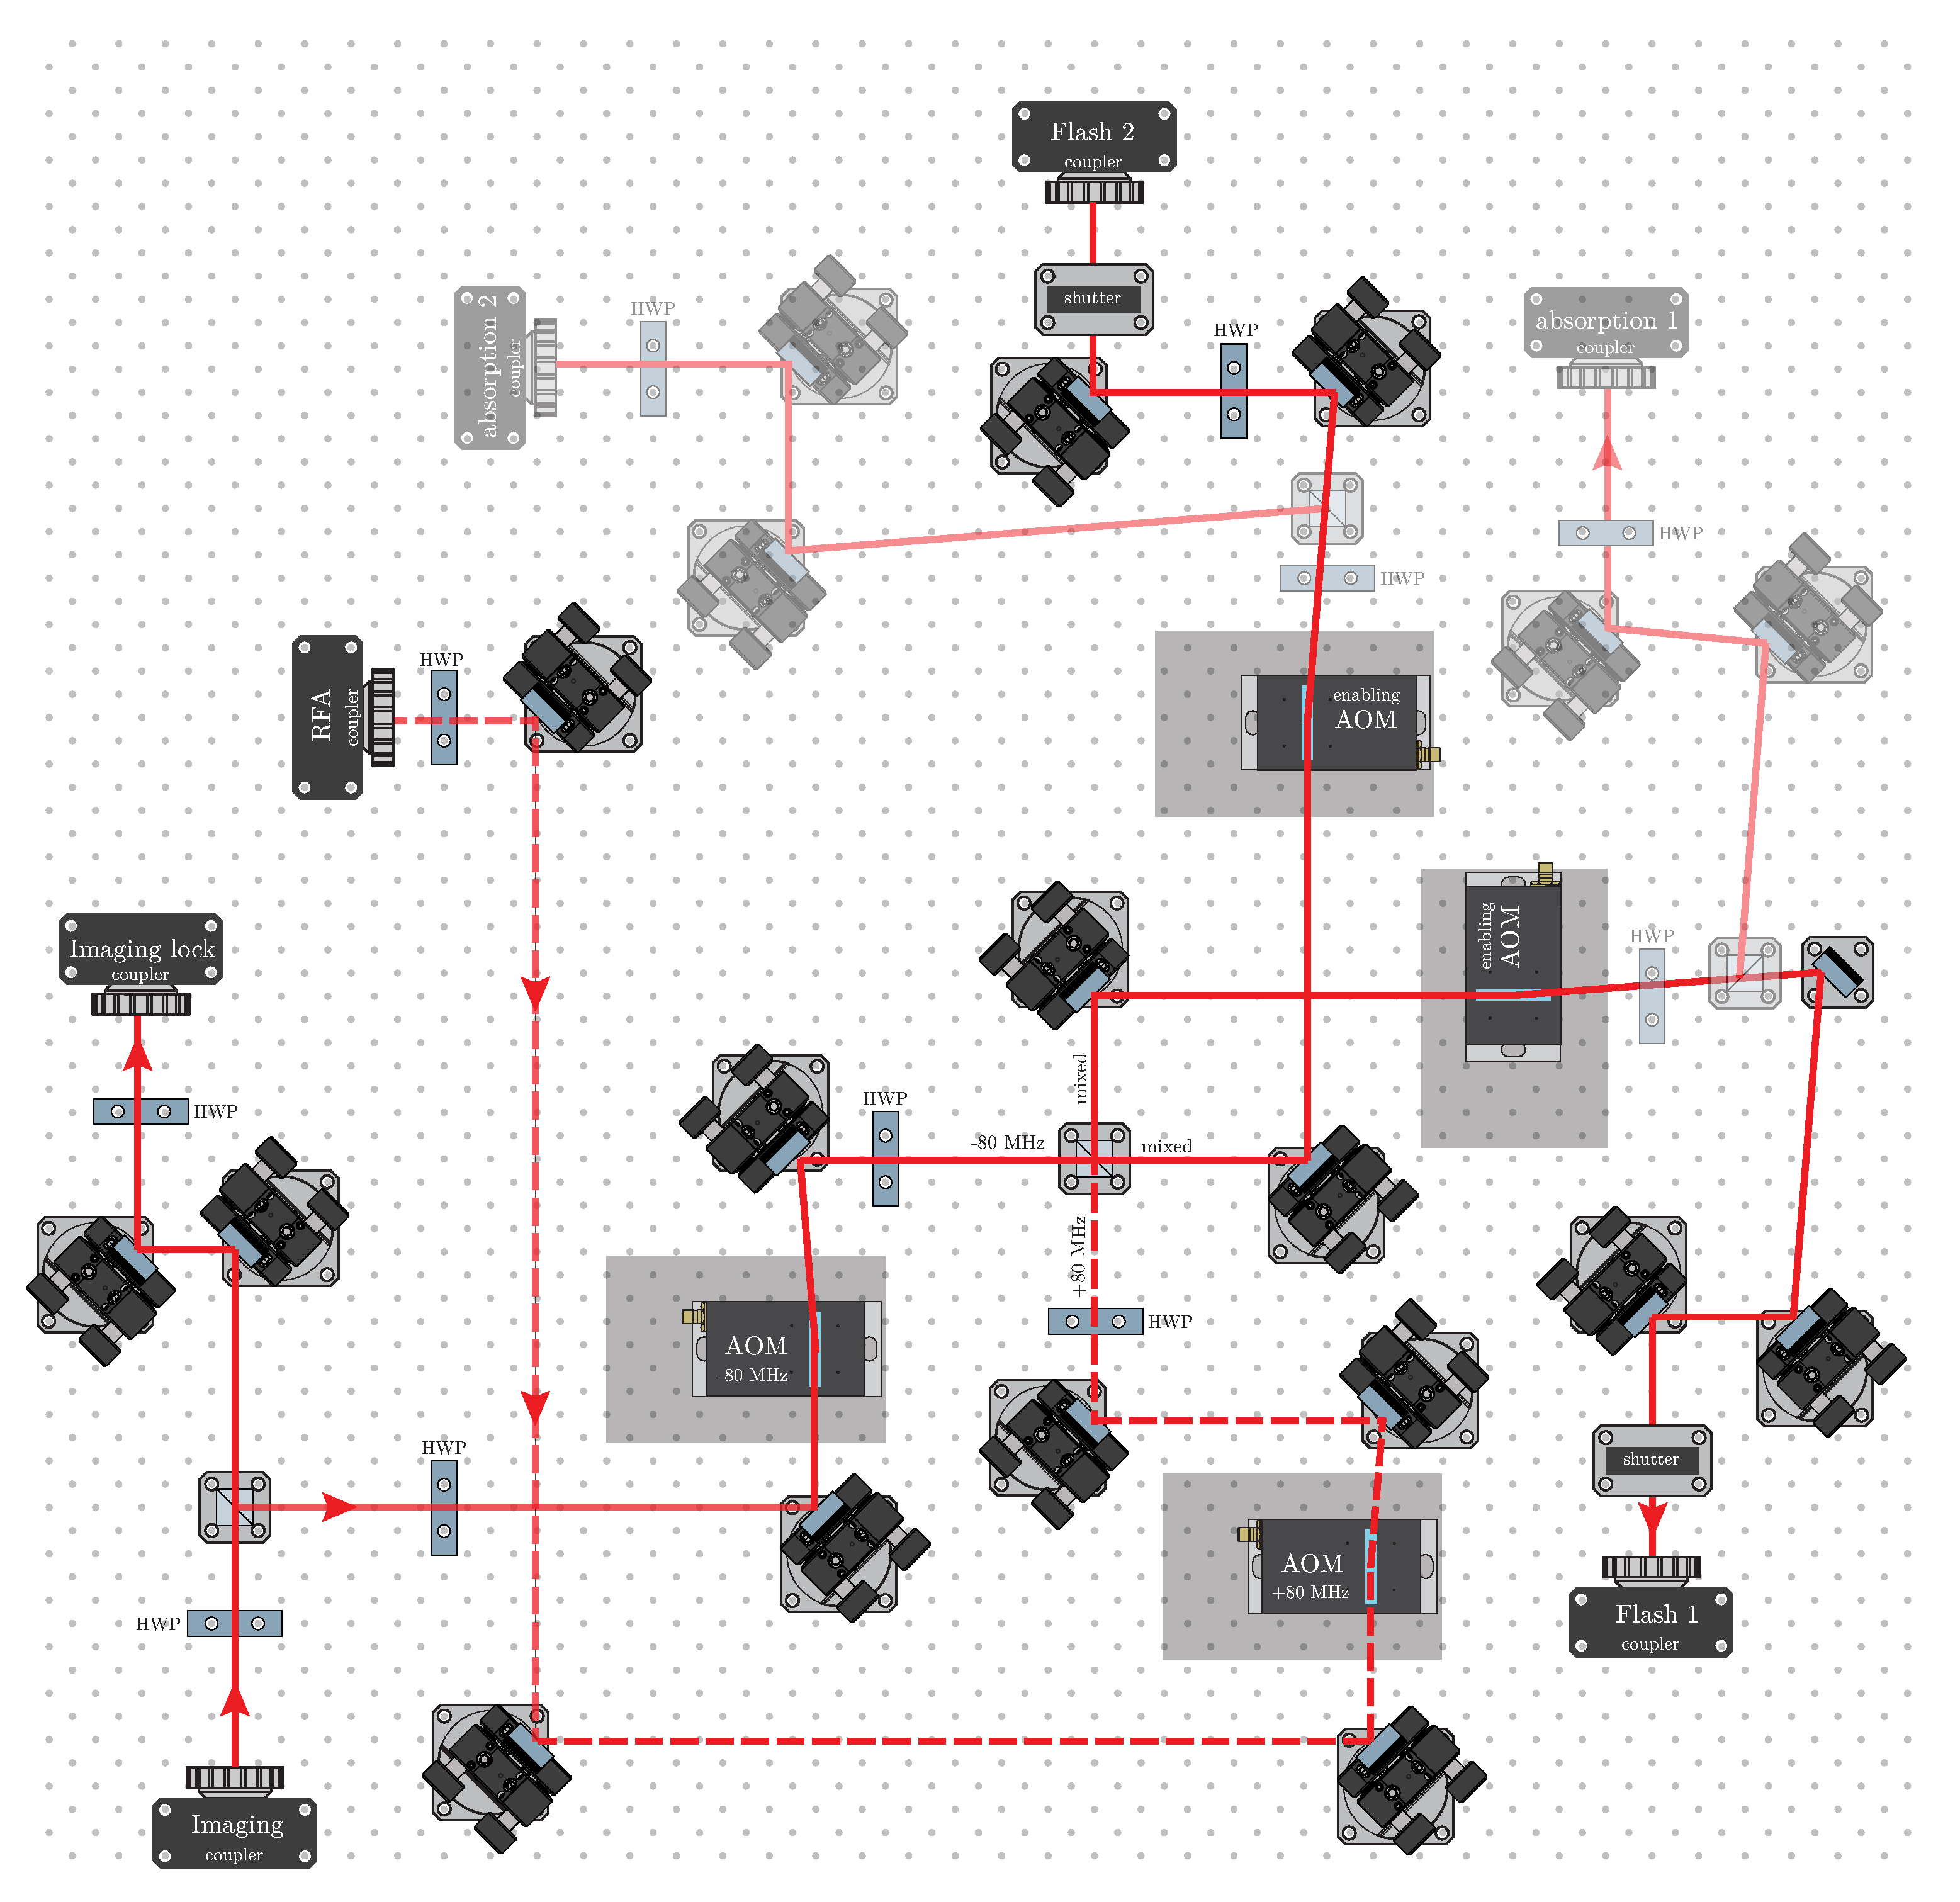
\includegraphics[width=0.4\textwidth]{fig-ai/flashing-distribution-scheme.pdf}
    \hspace{10 mm} 
    \addletter{195}{b} \phantom{4}
    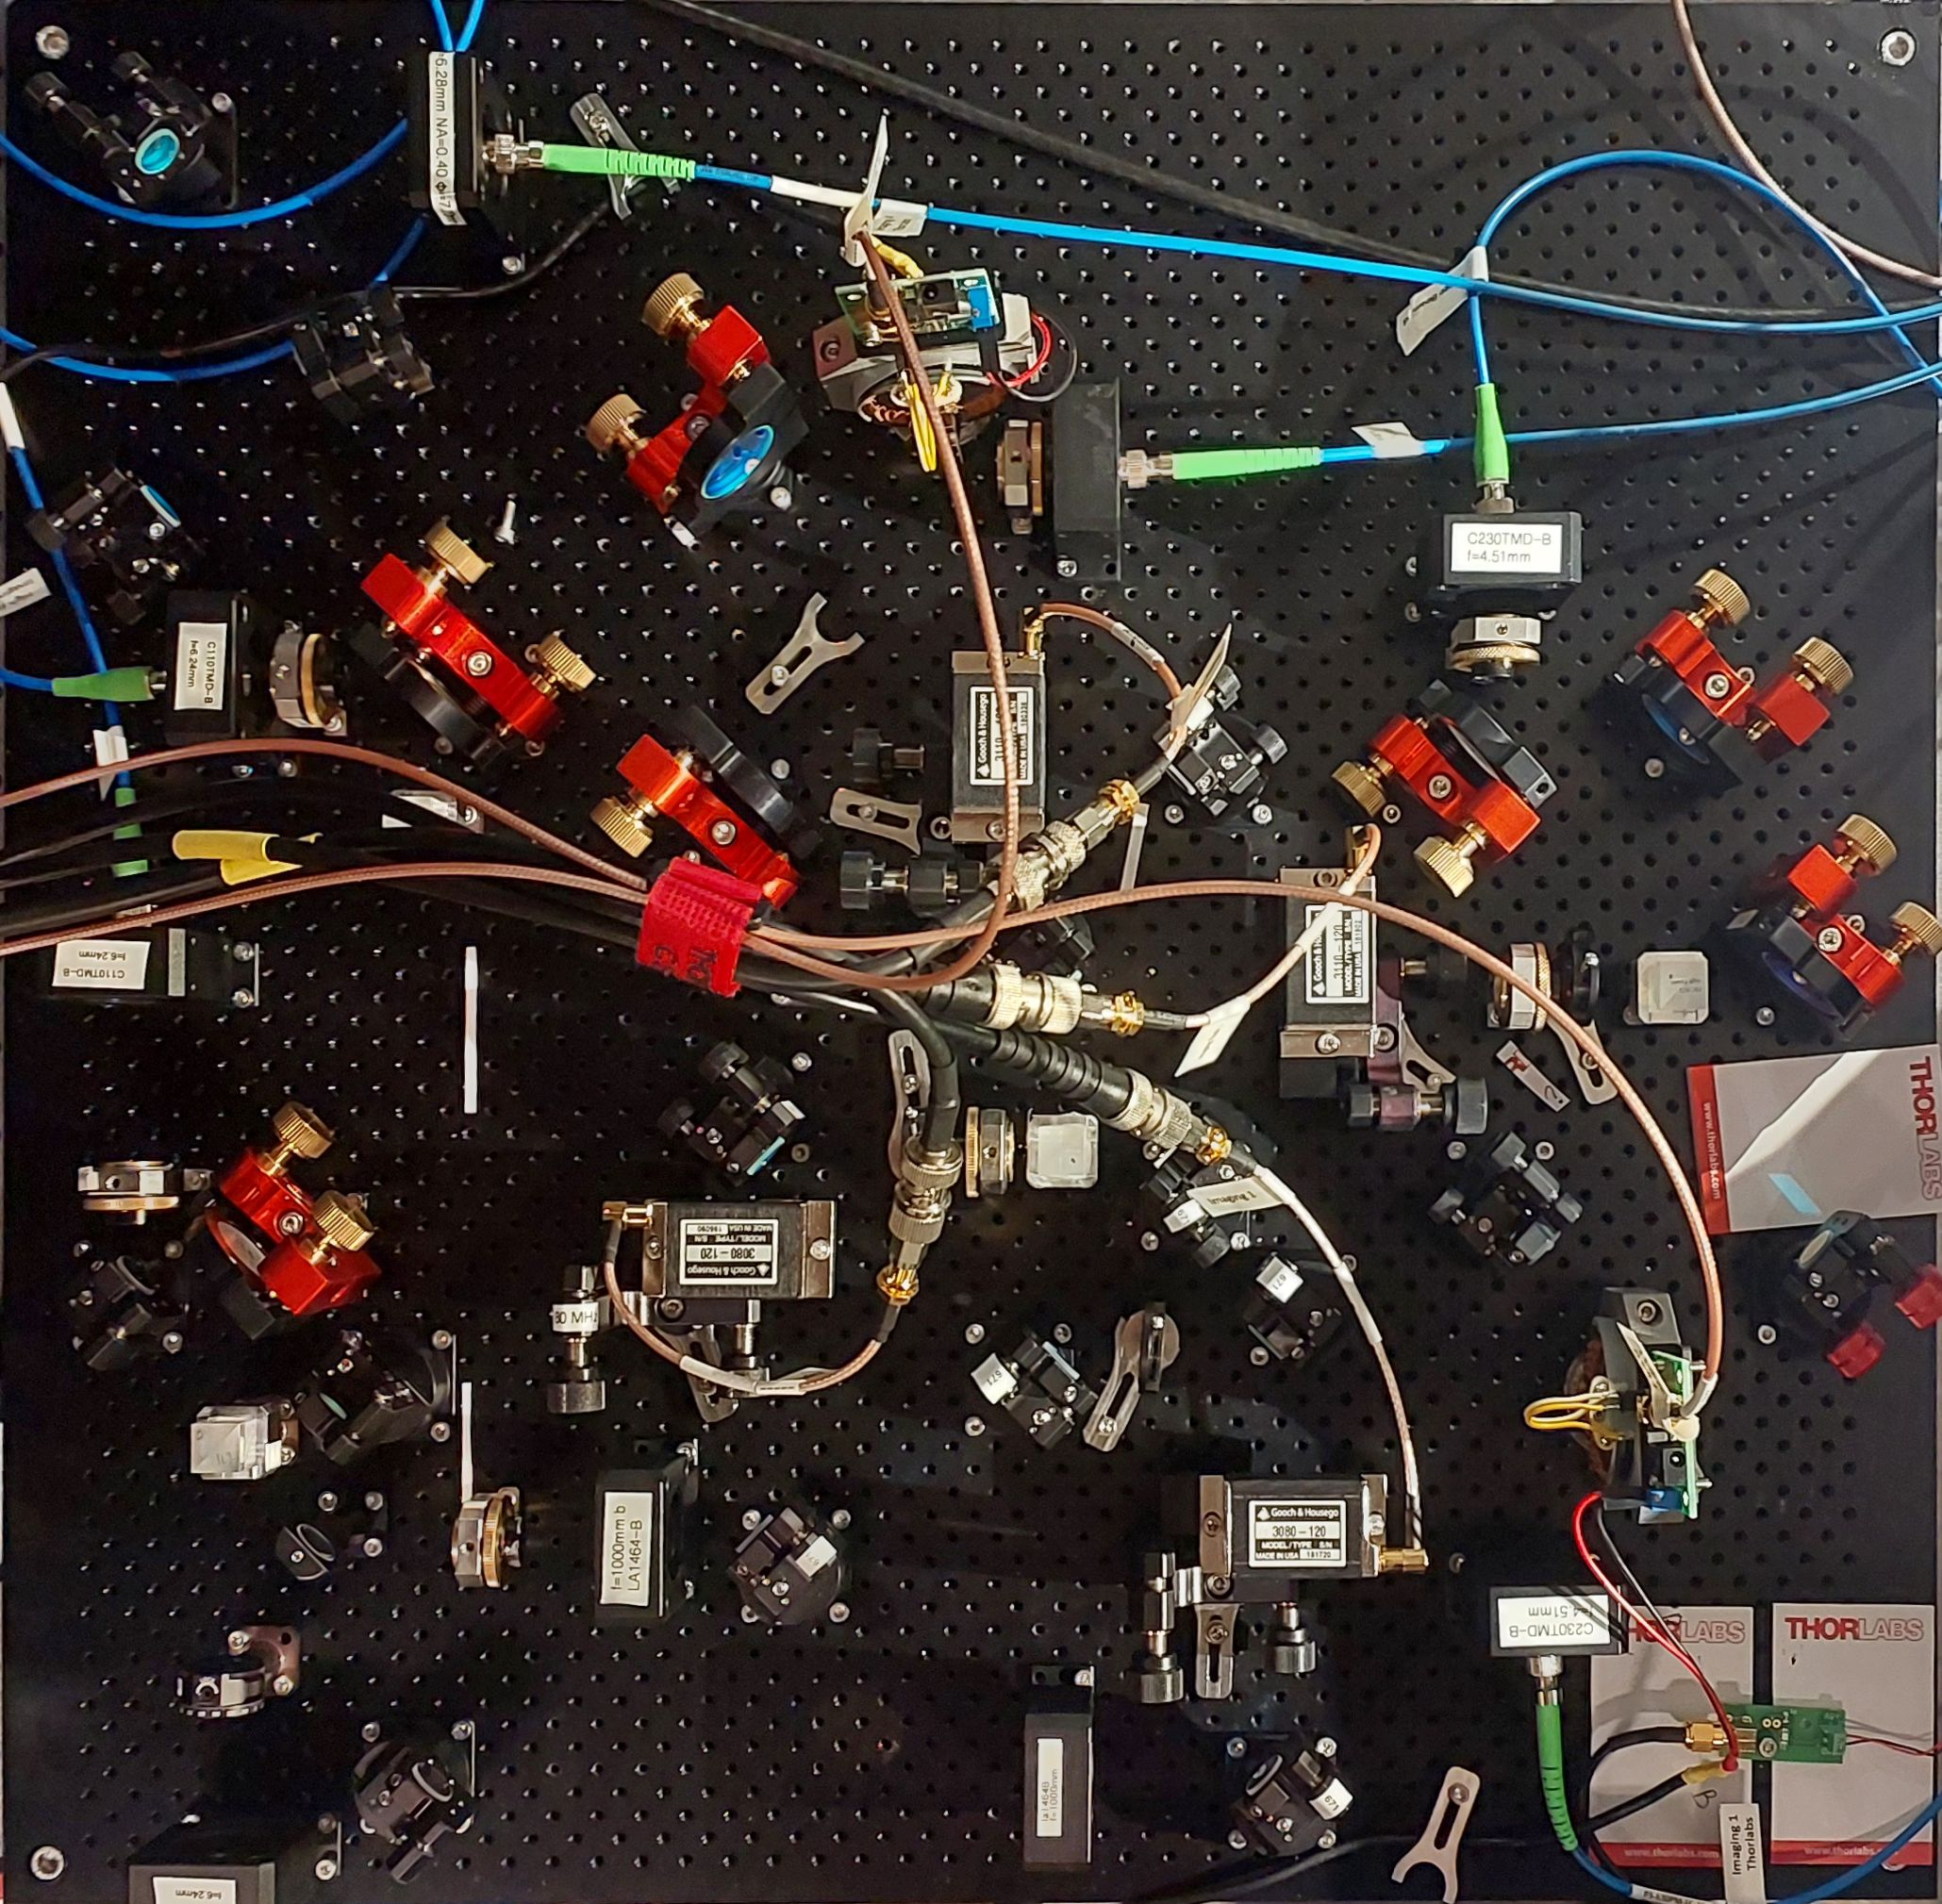
\includegraphics[width=0.4\textwidth]{imgs/flashing-distribution-img.jpg}

    \addletter{90}{c}
    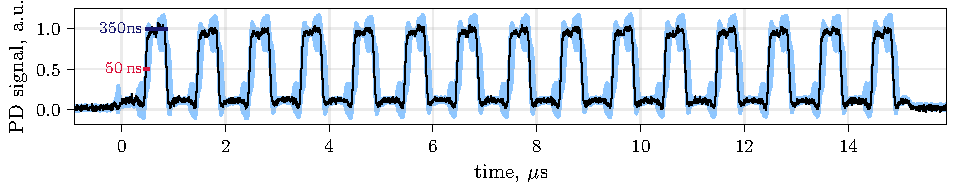
\includegraphics{fig-py/flashing-oscilloscope.pdf}

    \caption{
        \textbf{Distribution board for flashing}. 
        a) Optical layout of the board used to combine and control light for free-space imaging states $\ket{3}$ and $\ket{6}$.
        b) Experimental implementation.
        c) PD signal of the flashing measured on an oscilloscope (black -- a single experimental run, blue -- the standard deviation over 20 runs, red -- rise time).
    }
    \label{fig:flashing}
\end{figure}

\textbf{Beam combination and modulation.}  
The two lasers are routed through separate enabling AOMs (Gooch \& Housego 3080-120, 120 MHz), which act as fast shutters. The output beams are then combined on a non-polarizing beam splitter (nPBS), producing two spatially overlapping but frequency-distinct outputs. This combination stage is duplicated to form two independent paths, which are later used to illuminate the atoms from opposite directions. Each combined beam is sent through a dedicated flashing AOM (Gooch \& Housego 3080-120, 80 MHz), which controls the on-off modulation during imaging. The modulated light is then coupled into optical fibers, which deliver the light to the main experiment.

\textbf{Flashing control and synchronization.}  
To suppress recoil-induced diffusion (see Sec.~\ref{subsec:imaging-motivation}), the two beams are pulsed in an alternating sequence. This is achieved by driving the flashing AOMs with square-wave TTL signals at $1~\mathrm{MHz}$, generated by a Rigol waveform generator. The generator itself is triggered by the experimental sequencer (ADwin), ensuring precise timing with respect to the overall shot cycle. Since the imaging beams operate well into the saturation regime, no active power stabilization is required during the imaging sequence.

\textbf{Beam delivery and geometry.}  
Both beams are collimated and directed onto the atom plane from opposite sides. No focusing optics are used; the beams are weakly converging and approximately collimated over the imaging region. Polarizations are adjusted to match the required $\sigma^+$ or $\sigma^-$ conditions for selective excitation of $\ket{3}$ and $\ket{6}$. Fluorescence is collected through a high-numerical-aperture objective and split by a polarizing beam splitter (PBS), such that the $\sigma^+$ and $\sigma^-$ channels are imaged onto separate regions of the camera. This layout enables single-shot spin resolution (see Fig.~\ref{fig:spin-resolved} and Sec.~\ref{subsec:imaging-spin}).

\textbf{Implementation and contribution.}  
The distribution board for imaging and RFA beams (including combining optics, AOM stages, and fiber coupling) was fully designed and assembled in the course of this work. This included optical alignment of the two combined beam paths and flashing channels. The downstream delivery system, from fiber coupler to atom plane, was implemented in collaboration with other team members. The beam alignment to atoms was carried out by the author, ensuring symmetric illumination and proper polarization for spin-selective excitation.


--- imaging-spin.tex ---
% !TEX root = ../master-thesis.tex

\begin{figure}
    \centering
    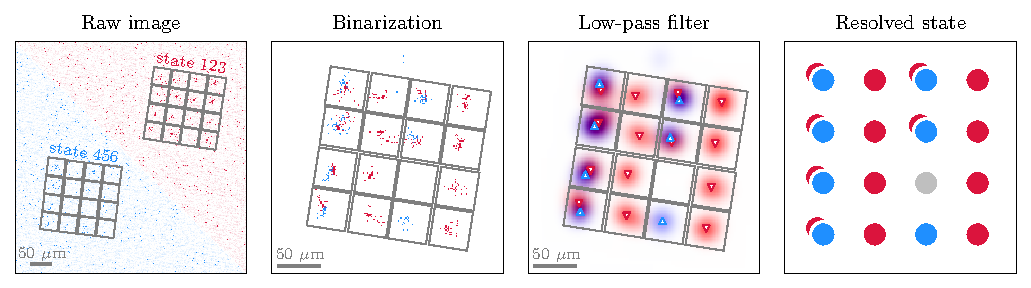
\includegraphics{fig-py/imaging-spin-resolved.pdf}
    \caption{
        \textbf{Spin-resolved single-atom imaging.}
        Spatially separated $\sigma_+$ and $\sigma_-$ fluorescence is imaged onto two distinct regions of the camera. The binarization step identifies photon counts above a threshold, followed by a low-pass filter to extract spatially localized signals. Final spin states are assigned based on relative signal strength in each channel:
        \raisebox{-1pt}{\scalebox{1.5}{\textcolor{ublue}{\textbullet}}} -- $\ket{1}$, 
        \raisebox{-1pt}{\scalebox{1.5}{\textcolor{ured}{\textbullet}}} -- $\ket{2}$, 
        \raisebox{-1pt}{\scalebox{1.5}{\textcolor{uhole}{\textbullet}}} -- no atom.
    }
    \label{fig:spin-resolved}
\end{figure}


\textbf{Single-shot spin resolution with spatial separation.}  
Spin detection is implemented through a single-exposure fluorescence measurement, where the emitted light from atoms in $\ket{3}$ and $\ket{6}$ is directed to different regions of the camera. This spatial separation is achieved using a polarizing beam splitter (PBS) after the imaging objective, which splits $\sigma^+$ and $\sigma^-$ components. In our geometry, atoms in state $\ket{3}$ produce fluorescence in the upper-right region of the frame, while those in $\ket{6}$ appear in the lower-left (see Fig.~\ref{fig:spin-resolved}). The system is calibrated so that each site in the tweezer array corresponds to two fixed analysis regions—one per spin channel.

\textbf{Filling detection.}  
For each tweezer site, the signal is integrated within two predefined ROIs, each capturing the fluorescence from one spin channel. The presence and identity of an atom is determined by comparing the signals from the two channels. If the signal in only one ROI exceeds a detection threshold, the corresponding spin state ($\ket{3}$ or $\ket{6}$) is assigned. If neither region contains sufficient signal, the site is identified as empty. If both channels yield strong and spatially localized peaks, this is interpreted as the presence of two atoms in different spin states at the same site.

\textbf{Fidelity estimation from single-atom preparation.}  
To characterize the performance of spin-resolved detection, we use deterministic state preparation. In these experiments, each tweezer contains an atom with a known spin state ($\ket{3}$ or $\ket{6}$) with approximately 95\% probability, as determined independently via fluorescence-based atom counting~\cite{dux_optical_2023}, see Fig.~\ref{fig:spillingadd}. Additionally, some choosen ROIs are intentionally left empty to provide ground truth data for evaluating false positive rates.

By applying the full detection pipeline to these experiments, we extract the rates of false positives (detecting an atom where none is present) and false negatives (failing to detect an atom where one exists). While the resulting classification accuracy depends on the overall filling fraction, the intrinsic detection characteristics (the false positive and false negative rates) are filling-independent. For a representative filling of 0.5, the resulting accuracy of spin-state assignment reaches 99\%. This performance level is sufficient for the current experiment stage.

\textbf{Implementation and contribution.}  
The complete processing pipeline for extracting spin-resolved occupancy data from camera images was implemented by the author. The classification algorithm builds on the same architecture used for unpolarized imaging but includes support for analyzing two spatially distinct fluorescence regions per site. The code is vectorized for efficient processing and can be extended to support additional spin channels or dynamic configurations.



--- intro.tex ---
% !TEX root = ../master-thesis.tex

\subsection{Quantum simulation with fermionic tweezer arrays}

The simulation of strongly correlated quantum systems remains one of the central challenges in modern physics. While exact numerical methods have provided deep insights in one-dimensional settings, the computational cost of simulating many-body dynamics in higher dimensions grows exponentially with system size, rendering classical approaches impractical. As first envisioned by Feynman, this motivates the development of physical quantum simulators that emulate target Hamiltonians using intrinsically quantum mechanical systems. Among several available platforms, ultracold atoms in optical potentials offer an exceptionally clean and versatile environment for realizing a broad range of many-body models, including the Fermi-Hubbard model relevant for high-temperature superconductivity~\cite{esslinger_fermi-hubbard_2010, gross_quantum_2017}.

In particular, fermionic atoms loaded into optical lattices have enabled the realization of the two-dimensional Fermi-Hubbard model, with site-resolved imaging revealing spin correlations and signatures of antiferromagnetic ordering~\cite{parsons_site-resolved_2016, boll_spin-_2016}. These advances highlight the power of quantum gas microscopy in exploring equilibrium properties of lattice fermions. However, conventional approaches rely on thermal loading of large ensembles into periodic potentials, which often results in uncontrolled entropy and random filling defects. As a consequence, the system is typically initialized in a thermal ensemble, and the preparation of arbitrary low-entropy many-body states remains difficult.

Optical tweezer arrays offer an alternative, bottom-up approach. By providing single-site control, they allow deterministic preparation of initial states, flexible geometries, and site-selective addressing. While initially developed in the context of Rydberg atom arrays~\cite{browaeys_many-body_2020}, these platforms have recently been extended to degenerate fermions, enabling programmable few-body Fermi-Hubbard dynamics~\cite{spar_realization_2022, yan_two-dimensional_2022}. Such results position tweezer arrays as a promising architecture for scalable fermionic quantum simulators.

This thesis contributes to the development of a quantum simulation platform based on ultracold fermionic $^6$Li atoms in a two-dimensional optical tweezer array. In this approach, the array is used for high-fidelity state preparation and control, while the optical lattice serves as the environment for Hamiltonian evolution. Compared to direct loading into a lattice, this separation of initialization and dynamics enables more efficient cooling, deterministic control over occupation patterns, and reduced cycle times. To support this workflow, we develop methods for spin-resolved free-space imaging, arbitrary pattern initialization via spin-selective spilling, and precise tweezer depth balancing.

Looking ahead, such a platform opens the door to nonequilibrium quantum dynamics. For instance, by performing randomized local operations followed by spin-resolved measurements, one can access entanglement entropy via measurement statistics~\cite{brydges_probing_2019}. These protocols offer a practical way to characterize entanglement growth and scrambling, even in regimes where full state tomography is infeasible. Extending such techniques to fermionic systems will provide new insights into thermalization, localization, and quantum information dynamics in strongly correlated matter.

In summary, this work supports the realization of a bottom-up fermionic quantum simulator by combining deterministic state preparation with single-atom, spin-resolved readout. These tools provide a foundation for studying both static and dynamical aspects of the Fermi-Hubbard model in a highly controlled setting.


\subsection{Thesis outline}

This thesis describes the development of experimental and computational tools for the preparation and probing of fermionic many-body states in a programmable optical tweezer array. The overarching goal is to enable bottom-up quantum simulation of lattice models, with precise control over initial conditions and single-atom, spin-resolved readout.

Sec.~\ref{sec:imaging} presents the implementation of spin-resolved single-atom imaging of $^6$Li in free space. The section describes the optical layout, the image processing pipeline, and introduces the Su-Schrieffer-Heeger model as a conceptual framework for understanding spin-dependent imaging dynamics.

Sec.~\ref{sec:tweezer} focuses on the creation and control of two-dimensional tweezer arrays. The section begins with the optical setup and AOD control, followed by a detailed discussion of calibration procedures and tweezer depth balancing using both camera-based and atom-based feedback. A key result is the development of a spin-selective spilling technique, enabling the preparation of spin- and site-resolved occupation patterns. Arbitrary configurations are realized through iterative removal steps, formalized via boolean matrix factorization.

Sec.~\ref{sec:mwm} introduces the concept of a matter-wave magnifier—a lensing scheme designed to enhance spatial resolution for future lattice imaging. Although not yet implemented experimentally, fast simulations of wavefunction propagation and Monte Carlo sampling are presented to validate the scheme.

Finally, Sec.~\ref{sec:fhmodel} outlines numerical approaches for simulating Fermi-Hubbard dynamics on small lattices. The computational framework combines exact diagonalization and Krylov-based time evolution, accelerated on GPU hardware. These tools enable simulations of dynamics in the presence of noise and disorder, and serve as a theoretical reference for upcoming experimental investigations.


% Sec.~\ref{sec:appendix} collects supporting material, including technical details of image processing and a description of the Boolean matrix factorization algorithm used for pattern optimization.



--- mwm-intro.tex ---
% !TEX root = ../master-thesis.tex

...

--- mwm-numerics.tex ---
% !TEX root = ../master-thesis.tex

...

--- notes.tex ---
% !TEX root = ../master-thesis.tex


\section*{Мысли про текст}

Ближайшие шаги:
\begin{enumerate}
	\item Описание unirand эксперимента
	\item Вводный рассказ про Fermi Hubbard
	\item Tweezer loading
	\item Tweezer movement
	\item ? MWM
	\item BMF as SAT task
	\item ? Написать про добавки к obj function в линейной модели
	
	% \item Atom based measurements: SVF, , atom-based crosstalk (and comparison)
	
	% \item site- and spin- resolved state preparation

	% \item non-factorizable state preparation, add large Li imgs (see movie)
	 % Можно а-ля the Li добавлять сверху к средним картинкам расшифровку

	% \item Графики для антенн с фитом

\end{enumerate}



\section*{Мысли про figures}


Можно добавить:
\begin{itemize}
	\item ! Схема стабилизации лазеров, какие отстройки, какие частоты, в контексте imaging
	% \item Single atom counting
	\item Демонстрация с Random Unitaries (Xinyi тезис)
	\item Схема установки, фото 3D mot
	% \item BEC
	\item Imaging: разница двух облачков (один, два continous, два alternating)
	% \item Imaging: histogram noise vs atoms, raw nuvu img
	% \item Flashing. Экспериментальная установка, табличка с её параметрами
	% \item State preparation: spilling. Схематичное изображение (посмотреть в Heidelberg thesis).
	% \item ? Экспериментальная последовательность
	\item ? Feshbach resonance
	% \item ? loading issues
	\item ? MWM (simulation, observed)
	\item ? Theory: описание fermi-hubbard, фазовая диаграмма (посмотреть coepsill)
	\item ? Theory: вклад от лабиринтов в локализацию
	% \item ? 2D Step Plot
\end{itemize}



% Huang: 17-25
% Culemann: 15-24




% Sec.\ref{sec:intro} or subsection\ref{subsec:control} Fig.\ref{fig:stepplot} or \eqref{eq:evolution}

--- occupation_control_tw_arr.tex ---
% !TEX root = ../master-thesis.tex

The ability to prepare arbitrary atom configurations is a key ingredient for bottom-up quantum simulation. After obtaining unit filling for both spin states (as discussed in Sec.~\ref{subsec:balancing} and \ref{subsec:spin-selective-spilling}), we implement a multi-stage spilling sequence that enables spin- and site-resolved initialization of arbitrary patterns.

The loading sequence proceeds in several steps:
\begin{enumerate*}
    \item Prepare a $\ket{1}$–$\ket{2}$ spin mixture with unit filling across the tweezer array.
    \item Perform global spilling steps to remove atoms from factorized intensity patterns $P_{ij}$, affecting both spin states.
    \item Apply spin-selective spilling steps to remove atoms in state $\ket{1}$ from additional factorized subsets of sites.
    \item Flip the remaining atoms $\ket{1} \leftrightarrow \ket{2}$ using a microwave $\pi$-pulse.
    \item Repeat spin-selective spilling to further refine the configuration
\end{enumerate*}

\textbf{Factorized removal.}
Each spilling step removes atoms from sites where the local tweezer depth $P_{ij}$ falls below a certain threshold. Since we can impose any rank-1 intensity mask $P_{ij} = H_i V_j$, it is possible to tailor the removal region to arbitrary product forms. To remove a single atom at site $(i', j')$, for example, we reduce $H_{i'}$ and $V_{j'}$ by a factor $\eta < 1$ and simultaneously increase the global power by $\eta$. This yields a relative intensity of $1/\eta$ at the intersection, while leaving all other sites unchanged or increased in depth. In this way, we can reliably isolate and remove atoms from any desired factorized subset.

\textbf{Boolean decomposition.}
We represent the cumulative removal pattern as a binary matrix $W_{ij}$, where $W_{ij} = 1$ indicates that the atom at site $(i, j)$ has been removed. Each spilling operation adds a binary outer product $u^\lambda_i v^\lambda_j$ via Boolean logic ($1 + 1 = 1$). An arbitrary target pattern can therefore be reached through a sequence of such operations:
\begin{equation}
    \label{eq:ebmf}
    W_{ij} = \bigvee_{\lambda=1}^{r} u^\lambda_i v^\lambda_j,
\end{equation}
which defines the exact Boolean matrix factorization (EBMF) of the removal matrix. In the worst case, any binary $n \times n$ matrix admits such a decomposition using at most $n$ steps.

\textbf{Optimal EBMF.}
While a naive strategy—such as row- or column-wise removal—may require up to $n$ iterations, we find that optimal EBMF often reduces this number. The problem of finding an exact Boolean matrix factorization with minimal rank is known to be NP-complete~\cite{orlin_contentment_1977} and NP-hard to approximate~\cite{gruber_inapproximability_2007}. Nevertheless, for arrays up to $10 \times 10$, optimal decompositions can be computed in a few seconds using a SAT solver. These improvements are particularly useful for minimizing experimental cycle time and improving overall sequence fidelity. A full discussion of the EBMF algorithm and its implementation is presented in Appendix.



--- prep_tw_arr.tex ---
% !TEX root = ../master-thesis.tex

% Тут хочется добавить общую последовательность эксперимента. То есть если говорю про imaging with flashing, добавим что происходит с магнитным полем и прочим важным (спросить Намана). Аналогично для state preparation, imaging.

% m: 40-42, 67-70
% h: 84-86, 


\begin{figure}
    \centering
    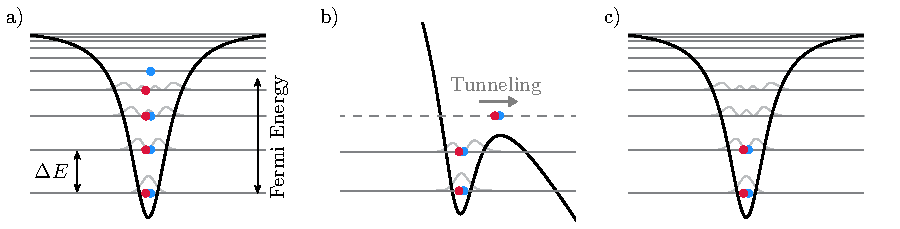
\includegraphics{fig-ai/preparation.pdf}
    \caption{
        \textbf{Deterministic preparation via spilling.}
        (a) Fermionic atoms are initially loaded into a tightly confined optical tweezer, forming a Fermi sea occupying the approximately 1D harmonic oscillator levels up to the Fermi energy. 
        (b) A magnetic field gradient tilts the potential, and the trap depth is lowered such that atoms above a defined spill level tunnel out. 
        (c) This procedure leaves a well-defined number of atoms in the lowest energy states, with a preparation fidelity of approximately 95\%. 
        Blue and red dots denote atoms in different spin states; gray curves indicate the bound-state wavefunctions.
    }
    \label{fig:preparation}
\end{figure}



\textbf{Tweezer loading.} We begin by preparing a spin-balanced mixture in the two lowest hyperfine states, $|1\rangle$ and $|2\rangle$, using a compressed magneto-optical trap (MOT). The atoms are initially loaded into a crossed ODT, where we perform evaporative cooling. This follows closely the sequence described in~\cite{culemann_construction_2024}.

After cooling, the atoms are transferred into a tightly focused optical tweezer potential. The loading process relies on the so-called \emph{dimple trick}~\cite{zurn_few-fermion_2012}, where a tightly confined but deep tweezer potential is superimposed onto the wider ODT reservoir. Because the tweezer affects only a small region of the total cloud, the global temperature $T$ remains approximately unchanged, while the local chemical potential is enhanced. In this regime, the average occupation number $\bar{n}(E_i)$ of a single-particle state $i$ with energy $E_i$ follows the Fermi-Dirac distribution:
\begin{equation}
    \bar{n}(E_i) = \frac{1}{e^{(E_i - \mu)/k_B T} + 1}.
\end{equation}
If the energy gap between the ground state $E_0$ and the Fermi energy $E_F$ is increased such that $(E_0 - E_F) / k_B \gg T$, then $\bar{n}(E_0) \rightarrow 1$. This ensures near-unity occupation of the lowest level, which provides an ideal starting point for deterministic preparation. In our experiment, this condition is achieved by ramping on the tweezer adiabatically while continuing evaporation inside the tweezer. The full loading and cooling sequence is depicted in Fig.~\ref{fig:preparationseq}.

\textbf{Deterministic few-body preparation via spilling.} To isolate a well-defined number of atoms in the lowest motional states of the tweezer, we use the \emph{spilling technique}, as described in~\cite{zurn_few-fermion_2012, holten_pauli_2022}. This method relies on tilting the potential with a magnetic field gradient and reducing the trap depth to allow atoms above a threshold energy to tunnel out. 
The resulting states are shown in Fig.~\ref{fig:preparation}. \red{See Appendix for details.}
% The energy levels and wavefunctions of the effective 1D potential under combined optical and magnetic fields were obtained numerically using a finite-difference method and the Thomas algorithm.

The spilling sequence is performed at a magnetic field of 527\,G, where the two spin states are nearly non-interacting. A magnetic field gradient of 20\,G/cm creates a linear tilt, and the tweezer power is lowered to a value that sets the spill threshold. After a short tunneling time, the trap depth is ramped back up to recapture the remaining atoms. By empirically optimizing these parameters, we achieve deterministic preparation of two atoms per tweezer with a fidelity of approximately 95\,\%. This sequence results in high-fidelity preparation within a total experimental cycle time of less than 2\,s.

% Стоит сказать, что система достаточно симметрична по отношению к уменьшению tweezer depth во время spilling или увеличению градиента. 


\begin{figure}
    \centering
    \addletter{140}{a}
    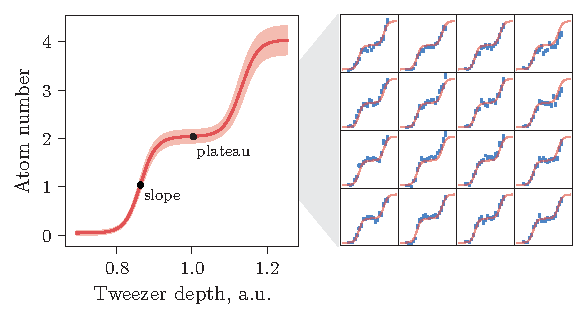
\includegraphics{fig-ai/step-plot-joined.pdf}
    \phantom{42}
    \addletter{140}{b}
    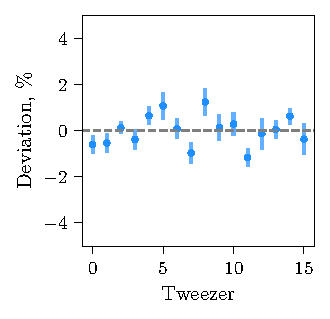
\includegraphics{fig-py/step-plot-balance.pdf} % 0.6 +- 0.2
    % 
    % 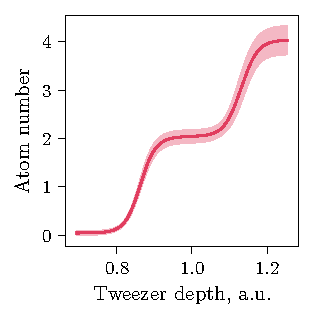
\includegraphics{fig-py/step-plot.pdf}
    % 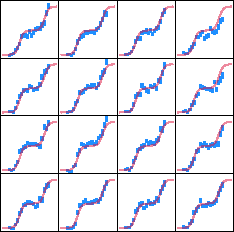
\includegraphics{fig-py/step-plot-inset.pdf}
    \caption{
        \textbf{Step plot.}
        (a) 
        Atom number as a function of tweezer depth during the spilling sequence. 
        % Plateaus correspond to quantized energy levels of the 1D harmonic oscillator. 
        Step plots for each tweezer in the $4 \times 4$ array are shown on the right. The average fit is shown as a solid red line, with standard deviation across sites indicated by the shaded area. 
        (b) Relative deviation of the fitted sigmoid centers for each tweezer after SVF balancing. The standard deviation is $0.7(2)\%$, which is well within the plateau width ($\pm 5\,\%$), ensuring sufficient uniformity for array-wide spilling. \red{$\chi^2$?}
        % All measurements were performed in this work using atom-based measurements and SVF-balanced tweezer depths.
    }
    \label{fig:stepplot}
\end{figure}

--- spin_spilling_tw_arr.tex ---
% !TEX root = ../master-thesis.tex

\begin{figure}
    \centering
    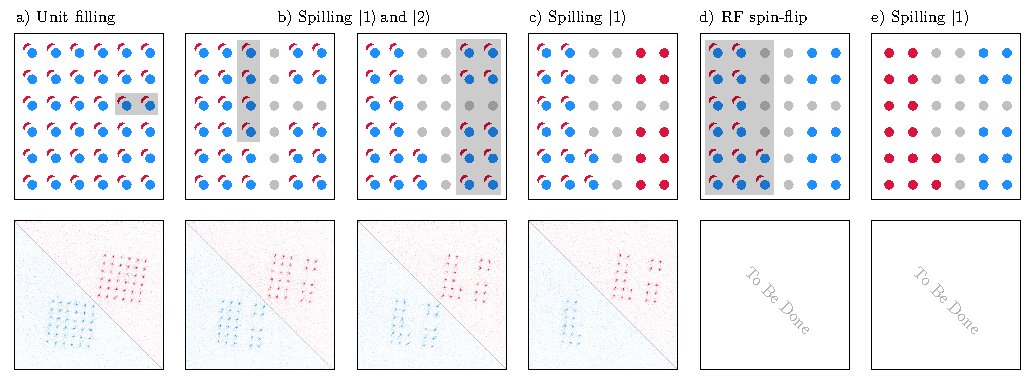
\includegraphics{fig-ai/preparation-array-ai.pdf}
    \caption{
    \textbf{Sequence for arbitrary filling preparation in a 2D tweezer array.}
    \textit{Top row}: Schematics of spin- and site-selective atom spilling, with gray shading indicating regions where atoms are removed. Blue and red semicircles represent atoms in different spin states, while gray circles denote emptied sites.
    \textit{Bottom row}: Experimental snapshots (averaged over 10 realizations) demonstrating each preparation stage. Panels (a)-(c) show completed experimental steps: initial unit filling (a), spilling of both spin states from selected regions (b), and spin-selective spilling of state $\ket{1}$ atoms (c). Panels (d)-(e) illustrate future planned steps, including spin-flip via RF transition (d) and subsequent spilling (e), which have not yet been experimentally realized.
    % due to pending hardware installation
    }
    \label{fig:preparation-array}
\end{figure}




After balancing the tweezer depths and performing standard spilling to prepare unit filling (one atom in state $\ket{1}$ and one in $\ket{2}$ per site), atoms in a selected spin state can be selectively removed while leaving the other unaffected. This enables the preparation of arbitrary spin-resolved configurations, a crucial ingredient for bottom-up simulation of spinful many-body systems.

\textbf{Magnetic-field dependence.}
The key idea relies on the difference in magnetic moments between the hyperfine ground states. As shown in Fig.~\ref{fig:li6levels}b, the energy of state $\ket{2}$ exhibits a maximum near $27\,\mathrm{G}$, where its magnetic moment vanishes: $\mu_{|2\rangle} = \partial E / \partial B = 0$. In contrast, state $\ket{1}$ has a sizable negative magnetic moment at this field \red{(write down value)}. As a result, when a magnetic field gradient is applied at $B = 27\,\mathrm{G}$, only atoms in state $\ket{1}$ experience a significant force and are spilled from the traps.

\textbf{Spin-selective removal.}
The experiment starts with a $\ket{1}$–$\ket{2}$ spin mixture at unit filling in each tweezer. The magnetic field is ramped to $27\,\mathrm{G}$, and a field gradient is applied. This results in spin-selective spilling: atoms in state $\ket{1}$ are removed, while those in $\ket{2}$ remain confined.

The crossed AOD configuration enables control over the local optical power $P_{ij}$ through factorized amplitudes, such that $P_{ij} = H_i V_j$. This allows us to define arbitrary rank-1 intensity masks and thus selectively apply spilling to specific subsets of sites. 
% In this way, we can prepare structured spin patterns such as stripes, checkerboards, or arbitrary factorized configurations.

This protocol enables single-shot removal of state $\ket{1}$ atoms without perturbing state $\ket{2}$, providing a flexible method for initializing spin-imbalanced or spatially patterned states. The performance of the method in terms of selectivity and overall fidelity is summarized in \red{Fig.~?}. Sequential applications of such steps to prepare arbitrary configurations are discussed in Sec.~\ref{subsec:arbitrary-occupation-loading}.


--- supplement.tex ---
% !TEX root = ../master-thesis.tex



--- tweezer-motivation.tex ---
% !TEX root = ../master-thesis.tex

\begin{figure}
    \centering
    % 
    \addletter{140}{a} 
    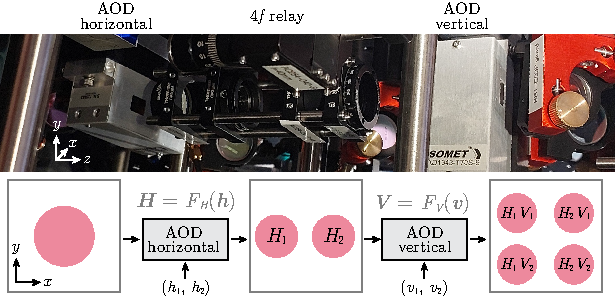
\includegraphics{fig-ai/crossed-aod.pdf}
    \hfill
    \addletter{140}{b} 
    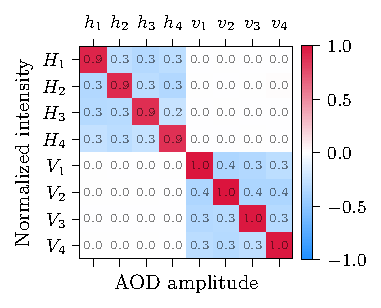
\includegraphics{fig-py/crosstalk-camera.pdf}
    % 
    \newline
    \phantom{42}
    \newline
    % 
    \addletter{115}{c}
    \raisebox{1cm}{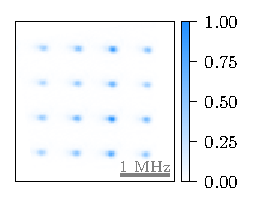
\includegraphics{fig-py/crosstalk-camera-img.pdf}}
    \phantom{42}
    \addletter{115}{d}
    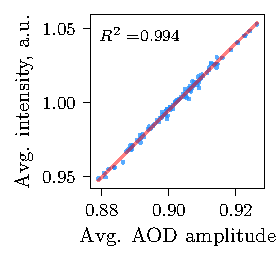
\includegraphics{fig-py/crosstalk-camera-amp.pdf}  
    \phantom{42}
    \addletter{115}{e}
    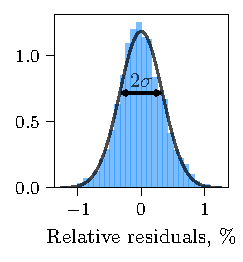
\includegraphics{fig-py/crosstalk-camera-res.pdf}
    % 
    \caption{
        \textbf{Tweezer array control using orthogonal AODs.}
        (a) Experimental setup: two orthogonal AODs generate a 2D tweezer array. The applied harmonic amplitudes $h_i$, $v_j$ define the output intensities $H_i = F_H(h)$ and $V_j = F_V(v)$ in horizontal and vertical directions, respectively. 
        (b) Crosstalk matrix $F'$ reconstructed via linear regression from camera images, showing how modulation of one harmonic affects others. 
        (c) Example of measured intensity distribution at uniform input amplitudes ($h_i = v_j = 0.9$), illustrating imbalance in the resulting pattern. 
        (d) The total intensity $\Lambda = \sum_{ij} H_i V_j$ scales linearly with the mean input amplitude. 
        (e) Residuals of the linear model (fitted in the range $[0.85, 0.95]$) are normally distributed. 
        All data were obtained in this work using direct camera-based measurements.
    }
    \label{fig:control}
\end{figure}


Optical tweezer arrays provide a flexible platform for preparing ultracold atomic systems with site-resolved control. By trapping individual atoms in focused laser beams, it becomes possible to initialize many-body states with controlled geometry, low entropy, and tunable local parameters.

In our setup, a two-dimensional array of tweezers is created using two orthogonal acousto-optic deflectors (AODs). Each AOD diffracts multiple beams along one axis, and their intersection forms the full array. The resulting intensity at site $(i,j)$ factorizes as $P_{ij} = H_i V_j$, where $H_i$ and $V_j$ are set by the drive amplitudes applied to each AOD. This structure simplifies calibration and allows fast control of the entire array using a small number of parameters.

Compared to holographic or lattice-based approaches, the AOD system offers rapid reconfigurability and independent control of individual traps. This enables preparation of custom spin and density patterns, as well as dynamic manipulation during the experimental sequence. Such capabilities are useful, for example, for initializing specific configurations, removing defects, or performing spatially selective operations before loading atoms into an optical lattice for further evolution.

\textbf{AOD operation.} Each AOD consists of a crystal driven by a piezoelectric transducer. An incoming laser beam $(\vc{k}_{\mathrm{in}}, \omega_{\mathrm{in}})$ interacts with the induced acoustic wave $(\vc{q}, \Omega)$ via Bragg diffraction, producing an outgoing beam $(\vc{k}_{\mathrm{out}}, \omega_{\mathrm{out}})$:
\begin{equation*}
    \vc{k}_{\mathrm{out}} = \vc{k}_{\mathrm{in}} + \vc{q}, \qquad \omega_{\mathrm{out}} = \omega_{\mathrm{in}} + \Omega.
\end{equation*}
The frequency $\Omega$ determines the deflection angle $\theta$ through the Bragg condition, while the amplitude of the RF signal controls the diffracted optical power. Each RF tone can be described by a triple $(\Omega_j, a_j, \varphi_j)$, corresponding to its frequency, amplitude, and phase. Applying a set of such tones to an AOD results in a superposition of multiple diffracted beams, with the amplitude $a_j$ determining the power in each beam and the phase $\varphi_j$ influencing their relative coherence.


\textbf{Factorized intensity distribution.} 
To create 2D arrays, we combine two AODs oriented along orthogonal axes (fig.~\ref{fig:control}a), as described in~\cite{culemann_construction_2024}.
Each axis is driven by a set of RF tones. In the paraxial approximation, the resulting 2D intensity pattern can be written as a rank-1 product of two vectors:
\begin{equation*}
    P_{ij} = H_i V_j,
\end{equation*}
where $H_i$ and $V_j$ correspond to the powers of individual beams generated by the horizontal and vertical AOD, respectively. The factorization of the output power can be verified via:
\begin{equation}
\label{eq:factorisability}
    P \overset{\mathrm{SVD}}{=} \textstyle \sum_r \Lambda_r \vc{H}_r \vc{V}_r\T,
    \hspace{10 mm} 
    \text{factorisability} = \Lambda_0 / \sum_r \Lambda_r 
\end{equation}
which provides a natural measure of factorization. For arrays ranging from $2\times2$ to $10\times10$, the factorisability measure $\Lambda_0 / \sum_r \Lambda_r$ is consistently above $0.99$. For the $4\times4$ array used in most of our experiments, we obtain a typical value of $0.997(1)$.

\textbf{Tweezer array control.} The tweezer output beam powers are nonlinear functions of the input amplitudes $\vc{a}$:
\begin{equation}
    \label{eq:taylerexp}
    P_j = F_j(\vc{a}) = \cancel{F_j(\vc{0})} + F'_{ji} a_i + \tfrac{1}{2} F''_{j i_1 i_2} a_{i_1} a_{i_2} + \ldots
\end{equation}
The goal is to control\footnote{
    For amplitudes in the range $a_i \in [0.7, 1.0]$, we find that a linear or quadratic approximation suffices. In practice, we reconstruct the Jacobian matrix $F'_{ji}$ using camera-based calibration, as discussed in Sec.~\ref{subsec:control}.
} the full matrix $P_{ij}$ using only two sets of parameters: horizontal amplitudes $\vc{h}$ and vertical amplitudes $\vc{v}$. 

It will later be necessary to reconstruct $(H_i, V_j)$ from measured intensity distribution $P_{ij}$, so it is convenient to choose a factorized model $P_{ij} = \Lambda H_i V_j$, with the normalization:
\begin{equation*}
    \sum_i H_i = \sum_j V_j = 1, \hspace{5 mm} \sum_{ij} P_{ij} = \Lambda.
\end{equation*}
This allows for an explicit decomposition:
\begin{equation}
    \textstyle
    \frac{1}{\Lambda} \sum_j P_{ij} = H_i \sum_j V_j = H_i,
    \hspace{5 mm} 
    \frac{1}{\Lambda} \sum_i P_{ij} = V_j \sum_i H_i = V_j,
    \hspace{5 mm} 
    \sum_{ij} P_{ij} = \Lambda,
    \label{uv-decomposition}
\end{equation}
which is fully equivalent to a rank-1 SVD of $P_{ij}$.

It is worth noting that, as shown in Fig.~\ref{fig:control}d, the total scale parameter $\Lambda$ defined in this way is proportional to the total input amplitude, $\sub{a}{sum} = \sum_j h_j + \sum_j v_j$. This effectively decouples local balancing from global power constraints, simplifying the control problem.

% \grey{This allows us to adjust the global scale $\Lambda$ (via a shared AOM or pre-AOD attenuation) and balance individual amplitudes using only two $n$-dimensional vectors.}


--- tweezer_loading.tex ---
% !TEX root = ../master-thesis.tex


\begin{figure}[h]
    \centering
    \addletter{90}{a}
    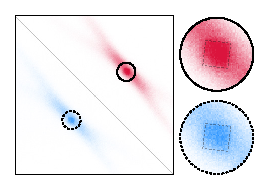
\includegraphics{fig-ai/loading-from-odt-1-ai.pdf}
    \phantom{42}
    \addletter{90}{b}
    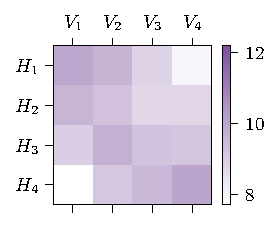
\includegraphics{fig-py/loading-from-odt-2.pdf}
    \phantom{42}
    \addletter{90}{c}
    \includegraphics{fig-py/loading-from-odt-3.pdf}
    \caption{
    \textbf{Inhomogeneous loading from ODT to tweezer arrays.}
    (a) Atom distribution for a $6\times6$ array (averaged over 10 realizations), demonstrating inhomogeneous loading from the optical dipole trap (ODT).
    (b) Observed atom number distribution for a uniformly powered $4\times4$ tweezer array, revealing systematically lower loading efficiency at corners (averaged over 30 realizations).
    (c) Improved uniformity after manual adjustment of tweezer intensities, specifically enhancing corner powers (averaged over 30 realizations).
    }
    \label{fig:loading-from-odt}
\end{figure}


--- tweezer_movement.tex ---
% !TEX root = ../master-thesis.tex

% tweezer_movement.tex

% \subsection{Tweezer movement} \label{subsec:tweezer-movement}

\begin{figure}[h]
\centering
\addletter{85}{a}
\includegraphics{fig-py/movement-inset.pdf} \\
\addletter{115}{b}
\includegraphics{fig-py/movement-1.pdf}
\hspace{1cm}
\addletter{115}{c}
\includegraphics{fig-py/movement-2.pdf}
\caption{
\textbf{Characterization of tweezer transport protocols.}
(a) Snapshots at different fractions of the total transport duration, illustrating atom movement between initial and target tweezer positions during a typical experimental run.
(b) Comparison of transport fidelity as a function of velocity for the Minimum-Jerk Trajectory (MJT) and linear trajectory. Fidelity is defined as the probability of detecting an atom after transport, conditional on its initial presence.
(c) Position versus time curves for MJT and linear transport trajectories.
Data points correspond to measurements, shaded areas represent standard deviation across realizations.
}
\label{fig:movement}
\end{figure}



\textbf{Tweezer movement}.
In experiments aiming at deterministic preparation and site-resolved imaging of individual ultracold atoms, precise and robust control over tweezer positions is crucial. In the present setup, while the Matter-Wave Magnifier (MWM) remains under development, single-atom imaging is achieved by initially positioning optical tweezers sufficiently far apart to individually resolve atoms. Specifically, atoms are loaded from the optical dipole trap (ODT) into tweezer potentials at an initial separation of $5,\mu$m. Subsequently, this spacing is gradually increased to approximately $50,\mu$m by smoothly varying the driving frequencies of the acousto-optic deflectors (AODs), enabling direct optical resolution without additional magnification.

\textbf{Transport trajectory optimization.}
The protocol chosen for tweezer translation critically influences the fidelity of atom transport. Naively, atoms can be moved by linearly ramping tweezer frequencies; however, such linear trajectories often lead to significant atom loss due to non-adiabatic excitations induced by abrupt changes in acceleration. To mitigate these losses, a smoother trajectory known as the Minimum-Jerk Trajectory (MJT) is employed. This trajectory is derived by minimizing the functional associated with the time-integrated square of the third derivative of the position, known as the jerk $j(t) = \dddot{x}(t)$:
\begin{equation}
\mathcal{J}[x(t)] = \int_{0}^{T} \left(\frac{d^3 x(t)}{dt^3}\right)^2 dt,
\label{eq:mjt-functional}
\end{equation}
where $x(t)$ denotes the position and $T$ the total transport duration. Minimization of Eq.~\eqref{eq:mjt-functional}, subject to the boundary conditions of initial and final positions $x(0) = x_i$, $x(T) = x_f$, and zero initial and final velocities and accelerations, yields a polynomial form:
\begin{equation}
x(t) = x_i + (x_f - x_i)\left[10\left(\frac{t}{T}\right)^3 - 15\left(\frac{t}{T}\right)^4 + 6\left(\frac{t}{T}\right)^5\right].
\label{eq:mjt-solution}
\end{equation}
This smooth polynomial interpolation minimizes abrupt changes in acceleration, thereby reducing non-adiabatic excitation and atom loss during transport.

\textbf{Experimental characterization of trajectories.}
To experimentally validate the efficacy of MJT compared to linear transport, systematic measurements were conducted. The fidelity of transport is defined as the probability of detecting an atom after transport, conditional upon its initial presence. As depicted in Fig.~\ref{fig:movement}b, the MJT significantly outperforms the linear trajectory across a broad range of transport velocities. These measurements are obtained by initially holding atoms stationary for a fixed duration, thereby establishing a baseline population expected without transport-induced losses. Subsequently, atoms are transported along a zigzag path (forward and backward), and transport fidelity is measured relative to this baseline.

Given the relatively low mass of lithium-6 atoms, high transport velocities are achievable. Indeed, at typical experimental transport velocities of approximately $10,\mu$m/ms, MJT achieves fidelities exceeding 99%, as demonstrated in Fig.~\ref{fig:movement}b. This highlights MJT as the trajectory of choice for efficient and robust tweezer movement.

\textbf{Trajectory profiles and experimental snapshots.}
Detailed position versus time curves for both linear and MJT trajectories are shown in Fig.\ref{fig:movement}c. The MJT profile distinctly smooths acceleration and deceleration phases compared to the linear ramp, clearly illustrating the reduction in jerk. Correspondingly, experimental snapshots at various fractions of the total transport duration, depicted in Fig.\ref{fig:movement}a, visually confirm smooth and uniform atomic redistribution between initial and final positions. Each snapshot represents fluorescence images averaged over ten experimental realizations, confirming reproducible atom transport without significant losses or heating.

In summary, the implementation and systematic characterization of MJT for tweezer translation provides a critical improvement in transport fidelity compared to simple linear movements. The derived and experimentally validated MJT ensures minimal atom loss, thereby facilitating precise atom arrangement required for subsequent experiments involving site- and spin-resolved imaging and manipulation.

